\documentclass[14pt]{extarticle}

\usepackage[table]{xcolor}
\usepackage{amsmath,mathtools,amsfonts,amsthm,amssymb,hyperref,wasysym,pifont}
\usepackage{parskip,geometry,latexsym,bookmark,mathtools,float,cancel,tcolorbox}

\newtheorem{defn}{Definition}
\newtheorem{thm}{Theorem}
\newtheorem{claim}{Claim}
\newtheorem{lemma}{Lemma}

\newcommand{\dps}{\displaystyle}
\newcommand{\fbl}{\underline{\hspace{1cm}}\,\,}
\newcommand{\R}{\mathbb{R}}
\newcommand{\Z}{\mathbb{Z}}
\newcommand{\from}{\leftarrow}
\newcommand{\true}{{\bf t}}
\newcommand{\false}{{\bf c}}
\newcommand{\bic}{\leftrightarrow}
\newcommand{\base}[1]{{\color{cyan}#1}}
\newcommand{\floor}[1]{{\left\lfloor#1\right\rfloor}}
\newcommand{\ceil}[1]{{\lceil#1\rceil}}
\newcommand{\da}{\downarrow}
\newcommand{\fa}{\forall}
\newcommand{\te}{\exists}
\newcommand{\cy}{\color{cyan}}

\newcommand{\colsq}[1]{{\color{#1} $\blacksquare$}}

\newcommand\Ccancel[2][black]{\renewcommand\CancelColor{\color{#1}}\cancel{#2}}
\newcommand\Cbcancel[2][black]{\renewcommand\CancelColor{\color{#1}}\bcancel{#2}}

\hypersetup{colorlinks,allcolors=blue,linktoc=all}
\geometry{a4paper}
\geometry{margin=0.42in}

\title{Chapter 5 Solutions, Susanna Epp Discrete Math 5th Edition}

\author{https://github.com/spamegg1}

\begin{document}
\maketitle
\tableofcontents

\section{Exercise Set 5.1}

{\bf \cy Write the first four terms of the sequences defined by the formulas in $1-6$.}

\subsection{Exercise 1}
$\dps a_k  = \frac{k}{10 + k}$, for every integer $k \geq 1$.

\begin{proof}
$\dps\frac{1}{11}, \frac{2}{12}, \frac{3}{13}, \frac{4}{14}$
\end{proof}

\subsection{Exercise 2}
$\dps b_j  = \frac{5-j}{5+j}$, for every integer $j \geq 1$.

\begin{proof}
$\dps\frac{4}{6}, \frac{3}{7}, \frac{2}{8}, \frac{1}{9}$
\end{proof}

\subsection{Exercise 3}
$\dps c_i  = \frac{(-1)^i}{3^i}$, for every integer $i \geq 0$.

\begin{proof}
$\dps 1, -\frac{1}{3}, \frac{1}{9}, -\frac{1}{27}$
\end{proof}

\subsection{Exercise 4}
$\dps d_m  = 1 + \left(\frac{1}{2}\right)^m$, for every integer $m \geq 0$.

\begin{proof}
$\dps 2, \frac{3}{2}, \frac{5}{4}, \frac{9}{8}$
\end{proof}

\subsection{Exercise 5}
$\dps e_n  = \floor{\frac{n}{2}}\cdot 2$, for every integer $n \geq 0$.

\begin{proof}
$0, 0, 2, 2$
\end{proof}

\subsection{Exercise 6}
$\dps f_n  = \floor{\frac{n}{4}}\cdot 4$, for every integer $n \geq 1$.

\begin{proof}
0, 0, 0, 4
\end{proof}

\subsection{Exercise 7}
Let $a_k = 2k + 1$ and $b_k = (k - 1)^3 + k + 2$ for every integer $k \geq 0$. Show that the first three terms of these sequences are identical but that their fourth terms differ.

\begin{proof}
$a_0 = 2(0) + 1 = 1, a_1 = 2(1) + 1 = 3, a_2 = 2(2) + 1 = 5, a_3 = 2(3) + 1 = 7$.

$b_0 = (0-1)^3 + 0 + 2 = 1, b_1 = (1-1)^3 + 1 + 2 = 3, b_2 = (2-1)^3 + 2 + 2 = 5, b_3 = (3-1)^3 + 3 + 2 = 13.$
\end{proof}

{\bf\cy Compute the first fifteen terms of each of the sequences in 8 and 9, and describe the general behavior of these sequences in words. (a definition of logarithm is given in Section 7.1.)}

\subsection{Exercise 8}
$g_n = \floor{\log_2 n}$ for every integer $n \geq 1$.

\begin{proof}
$g_1 = \floor{\log_2 1} = 0, g_2 = \floor{\log_2 2} = 1, g_3 = \floor{\log_2 3} = 1, g_4 = \floor{\log_2 4} = 2$,

$g_5 = \floor{\log_2 5} = 2, g_6 = \floor{\log_2 6} = 2, g_7 = \floor{\log_2 7} = 2, g_8 = \floor{\log_2 8} = 3$, 

$g_9 = \floor{\log_2 9} = 3, g_{10} = \floor{\log_2 10} = 3, g_{11} = \floor{\log_2 11} = 3, g_{12} = \floor{\log_2 12} = 3$, 

$g_{13} = \floor{\log_2 13} = 3, g_{14} = \floor{\log_2 14} = 3, g_{15} = \floor{\log_2 15} = 3$.

When $n$ is an integral power of 2, $g_n$ is the exponent of that power. For instance, $8 = 2^3$ and $g_8 = 3$. More generally, if $n = 2k$, where $k$ is an integer, then $g_n = k$. All terms of the sequence from $g_{2^k}$ up to, but not including, $g_{2^{k+1}}$ have the same value, namely $k$. For instance, all terms of the sequence from $g_8$ through $g_{15}$ have the value 3.
\end{proof}

\subsection{Exercise 9}
$h_n = n\floor{\log_2 n}$ for every integer $n \geq 1$.

\begin{proof}
$h_1 = 1\floor{\log_2 1} = 0, h_2 = 2\floor{\log_2 2} = 2, h_3 = 3\floor{\log_2 3} = 3, h_4 = 4\floor{\log_2 4} = 8$,

$h_5 = 5\floor{\log_2 5} = 10, h_6 = 6\floor{\log_2 6} = 12, h_7 = 7\floor{\log_2 7} = 14, h_8 = 8\floor{\log_2 8} = 24$, 

$h_9 = 9\floor{\log_2 9} = 27, h_{10} = 10\floor{\log_2 10} = 30, h_{11} = 11\floor{\log_2 11} = 33$, 

$h_{12} = 12\floor{\log_2 12} = 36, h_{13} = 13\floor{\log_2 13} = 39, h_{14} = 14\floor{\log_2 14} = 42,$ 

$h_{15} = 15\floor{\log_2 15} = 45$.
\end{proof}

{\bf\cy Find explicit formulas for sequences of the form $a_1, a_2, a_3, \ldots$ with the initial terms given in $10-16$.}

{\bf\cy Exercises $10-16$ have more than one correct answer.}

\subsection{Exercise 10}
$-1, 1, -1, 1, -1, 1$

\begin{proof}
$a_n = (-1)^n$, where $n$ is an integer and $n \geq 1$
\end{proof}

\subsection{Exercise 11}
$0, 1, -2, 3, -4, 5$

\begin{proof}
$a_n = (n-1)(-1)^n$, where $n$ is an integer and $n \geq 1$
\end{proof}

\subsection{Exercise 12}
$\dps \frac{1}{4}, \frac{2}{9}, \frac{3}{16}, \frac{4}{25}, \frac{5}{36}, \frac{6}{49}$

\begin{proof}
$\dps a_n = \frac{n}{(n+1)^2}$, where $n$ is an integer and $n \geq 1$
\end{proof}

\subsection{Exercise 13}
$\dps 1 - \frac{1}{2}, \frac{1}{2} - \frac{1}{3}, \frac{1}{3} - \frac{1}{4}, \frac{1}{4} - \frac{1}{5}, \frac{1}{5} - \frac{1}{6}, \frac{1}{6} - \frac{1}{7}$

\begin{proof}
$\dps a_n = \frac{1}{n} - \frac{1}{n+1}$, where $n$ is an integer and $n \geq 1$
\end{proof}

\subsection{Exercise 14}
$\dps \frac{1}{3}, \frac{4}{9}, \frac{9}{27}, \frac{16}{81}, \frac{25}{243}, \frac{36}{729}$

\begin{proof}
$\dps a_n = \frac{n^2}{3^n}$, where $n$ is an integer and $n \geq 1$
\end{proof}

\subsection{Exercise 15}
$\dps 0, -\frac{1}{2}, \frac{2}{3}, -\frac{3}{4}, \frac{4}{5}, -\frac{5}{6}, \frac{6}{7}$

\begin{proof}
$\dps a_n = \frac{n-1}{n}\cdot(-1)^{n-1}$, where $n$ is an integer and $n \geq 1$
\end{proof}

\subsection{Exercise 16}
3, 6, 12, 24, 48, 96

\begin{proof}
$\dps a_n = 3\cdot 2^{n-1}$, where $n$ is an integer and $n \geq 1$
\end{proof}

\subsection{Exercise 17}
Consider the sequence defined by $\dps a_n = \frac{2n + (-1)^n - 1}{4}$ for every integer $n \geq 0$. Find an alternative explicit formula for an that uses the floor notation.

\begin{proof}
$a_0 = 0, a_1 = 0, a_2 = 1, a_3 = 1, a_4 = 2, a_5 = 2$. It seems to be following the pattern: $\dps a_n = \floor{\frac{n}{2}}$. Let's try to prove this. When $n$ is even, $n = 2k$ for some integer $k$, so we have
\[
a_n = a_{2k} = \frac{2(2k) + (-1)^{2k} - 1}{4} = \frac{4k + 1 - 1}{4} = \frac{4k}{4} = k = \frac{n}{2} = \floor{\frac{n}{2}}
\]
When $n$ is odd, $n = 2k+1$ for some integer $k$, so we have
\[
a_n = a_{2k+1} = \frac{2(2k+1) + (-1)^{2k+1} - 1}{4} = \frac{4k + 2 - 1 - 1}{4} = \frac{4k}{4} = k = \frac{n-1}{2} = \floor{\frac{n}{2}}
\]
So $\dps a_n = \floor{\frac{n}{2}}$ for all $n \geq 0$.
\end{proof}

\subsection{Exercise 18}
Let $a_0 = 2, a_1 = 3, a_2 = -2, a_3 = 1, a_4 = 0, a_5 = -1$, and $a_6 = -2$. Compute each of the summations and products below.

\subsubsection{(a)}
$\dps\sum_{i=0}^{6}a_i$

\begin{proof}
$2 + 3 + (-2) + 1 + 0 + (-1) + (-2) = 1$

\end{proof}

\subsubsection{(b)}
$\dps\sum_{i=0}^{0}a_i$

\begin{proof}
$a_0 = 2$
\end{proof}

\subsubsection{(c)}
$\dps\sum_{j=1}^{3}a_{2j}$

\begin{proof}
$a_2 + a_4 + a_6 = -2 + 0 + (-2) = -4$
\end{proof}

\subsubsection{(d)}
$\dps\prod_{k=0}^{6}a_k$

\begin{proof}
$2 \cdot 3 \cdot (-2) \cdot 1 \cdot 0 \cdot (-1) \cdot (-2) = 0$
\end{proof}

\subsubsection{(e)}
$\dps\prod_{k=2}^{2}a_k$

\begin{proof}

\end{proof}

{\bf\cy Compute the summations and products in $19-28$.}

\subsection{Exercise 19}
$\dps\sum_{k=1}^{5}(k+1)$

\begin{proof}
$2+3+4+5+6=20$
\end{proof}

\subsection{Exercise 20}
$\dps\prod_{k=2}^{4}{k}^2$

\begin{proof}
$2^2\cdot 3^2\cdot 4^2 = 576$
\end{proof}

\subsection{Exercise 21}
$\dps\sum_{k=1}^{3}(k^2+1)$

\begin{proof}
$(1^2+1) + (2^2+1) + (3^2+1) = 2+5+10 = 17$
\end{proof}

\subsection{Exercise 22}
$\dps\prod_{j=0}^{4}{(-1)}^j$

\begin{proof}
$(-1)^0\cdot (-1)^1\cdot (-1)^2\cdot (-1)^3\cdot(-1)^4 = 1$
\end{proof}

\subsection{Exercise 23}
$\dps\sum_{i=1}^{1}i(i+1)$

\begin{proof}
1(1+1) = 2
\end{proof}

\subsection{Exercise 24}
$\dps\sum_{j=0}^{0}(j+1)\cdot2^j$

\begin{proof}
$(0+1)\cdot 2^0 = 1$
\end{proof}

\subsection{Exercise 25}
$\dps\prod_{k=2}^{2}\left(1 - \frac{1}{k}\right)$

\begin{proof}
$(1 - 1/2) = 1/2$
\end{proof}

\subsection{Exercise 26}
$\dps\sum_{k=-1}^{1}(k^2+3)$

\begin{proof}
$((-1)^2+3) + (0^2+3) + (1^2+3) = 11$
\end{proof}

\subsection{Exercise 27}
$\dps\sum_{n=1}^{6}\left(\frac{1}{n} - \frac{1}{n+1}\right)$

\begin{proof}
$\dps \left(\frac{1}{1} - \Ccancel[cyan]{\frac{1}{2}}\right) + \left(\Ccancel[cyan]{\frac{1}{2}} - \Ccancel[red]{\frac{1}{3}}\right) + \left(\Ccancel[red]{\frac{1}{3}} - \Ccancel[green]{\frac{1}{4}}\right) + \left(\Ccancel[green]{\frac{1}{4}} - \Ccancel[magenta]{\frac{1}{5}}\right) + \left(\Ccancel[magenta]{\frac{1}{5}} - \Ccancel[black]{\frac{1}{6}}\right) + \left(\Ccancel[black]{\frac{1}{6}} - \frac{1}{7}\right)$

$\dps = 1 - \frac{1}{7} = \frac{6}{7}$
\end{proof}

\subsection{Exercise 28}
$\dps\prod_{i=2}^{5}\frac{i(i+2)}{(i-1)\cdot(i+1)}$

\begin{proof}
$\dps \frac{2(2+2)}{(2-1)(2+1)}\cdot\frac{3(3+2)}{(3-1)(3+1)}\cdot\frac{4(4+2)}{(4-1)(4+1)}\cdot\frac{5(5+2)}{(5-1)(5+1)}$

$\dps = \frac{\Ccancel[cyan]{8}}{3}\cdot\frac{\Ccancel[red]{15}}{\Ccancel[cyan]{8}}\cdot\frac{\Ccancel[green]{24}}{\Ccancel[red]{15}}\cdot\frac{35}{\Ccancel[green]{24}}\cdot = \frac{35}{3}$
\end{proof}

{\bf\cy Write the summations in $29-32$ in expanded form.}

\subsection{Exercise 29}
$\dps\sum_{i=1}^{n}(-2)^i$

\begin{proof}
$(-2)^1 + (-2)^2 + (-2)^3 + \cdots + (-2)^n = -2 + 2^2 - 2^3 + \cdots + (-1)^n2^n$
\end{proof}

\subsection{Exercise 30}
$\dps\sum_{j=1}^{n}j(j+1)$

\begin{proof}
$1\cdot2 + 2\cdot3 + 3\cdot4 + \cdots + n(n+1)$
\end{proof}

\subsection{Exercise 31}
$\dps\sum_{k=0}^{n+1}\frac{1}{k!}$

\begin{proof}
$\dps\sum_{k=0}^{n+1}\frac{1}{k!} = \frac{1}{0!} + \frac{1}{1!} + \frac{1}{2!} + \cdots + \frac{1}{(n+1)!}$
\end{proof}

\subsection{Exercise 32}
$\dps\sum_{i=1}^{k+1}i(i!)$

\begin{proof}
$1(1!) + 2(2!) + 3(3!) + \cdots + (k+1)(k+1)!$
\end{proof}

{\bf\cy Evaluate the summations and products in $33-36$ for the indicated values of the variable.}

\subsection{Exercise 33}
$\dps \frac{1}{1^2} + \frac{1}{2^2} + \frac{1}{3^2} + \cdots + \frac{1}{n^2}$; $n = 1$

\begin{proof}
$\dps\frac{1}{1^2} = 1$
\end{proof}

\subsection{Exercise 34}
$\dps 1(1!) + 2(2!) + 3(3!) + \cdots + m(m!)$; $m = 2$

\begin{proof}
$\dps 1(1!) + 2(2!) = 1 + 4 = 5$
\end{proof}

\subsection{Exercise 35}
$\dps \left(\frac{1}{1+1}\right)\left(\frac{2}{2+1}\right)\left(\frac{3}{3+1}\right) \cdots \left(\frac{k}{k+1}\right)$; $k = 3$

\begin{proof}
$\dps \left(\frac{1}{1+1}\right)\left(\frac{2}{2+1}\right)\left(\frac{3}{3+1}\right) = \frac{1}{2}\frac{2}{3}\frac{3}{4} = \frac{1}{4}$
\end{proof}

\subsection{Exercise 36}
$\dps \left(\frac{1\cdot2}{3\cdot4}\right)\left(\frac{2\cdot3}{4\cdot5}\right)\left(\frac{3\cdot4}{5\cdot6}\right)\cdots\left(\frac{m\cdot(m+1)}{(m+2)\cdot(m+3)}\right); m = 1$

\begin{proof}
$\dps \frac{1\cdot2}{3\cdot4} = \frac{3}{8}$
\end{proof}

{\bf\cy Write each of $37-39$ as a single summation.}

\subsection{Exercise 37}
$\dps\sum_{i=1}^{k}i^3 + (k+1)^3$

\begin{proof}
$\dps\sum_{i=1}^{k+1}i^3$
\end{proof}

\subsection{Exercise 38}
$\dps\sum_{k=1}^{m}\frac{k}{k+1} + \frac{m+1}{m+2}$

\begin{proof}
$\dps\sum_{k=1}^{m+1}\frac{k}{k+1}$
\end{proof}

\subsection{Exercise 39}
$\dps\sum_{m=0}^{n}(m+1)2^n + (n+2)2^{n+1}$

\begin{proof}
$\dps\sum_{m=0}^{n+1}(m+1)2^n$
\end{proof}

{\bf\cy Rewrite $40-42$ by separating off the final term.}

\subsection{Exercise 40}
$\dps\sum_{i=1}^{k+1}i(i!)$

\begin{proof}
$\dps\sum_{i=1}^{k}i(i!) + (k+1)(k+1)!$
\end{proof}

\subsection{Exercise 41}
$\dps\sum_{k=1}^{m+1}k^2$

\begin{proof}
$\dps\sum_{k=1}^{m}k^2 + (m+1)^2$
\end{proof}

\subsection{Exercise 42}
$\dps\sum_{m=1}^{n+1}m(m+1)$

\begin{proof}
$\dps\sum_{m=1}^{n}m(m+1) + (n+1)(n+2)$
\end{proof}

{\bf\cy Write each of $43-52$ using summation or product
notation.}

{\bf\cy Exercises $43-52$ have more than one correct answer.}

\subsection{Exercise 43}
$1^2 - 2^2 + 3^2 - 4^2 + 5^2 - 6^2 + 7^2$

\begin{proof}
$\dps \sum_{k=1}^{7}(-1)^{k+1}k^2$ or $\dps \sum_{k=0}^{6}(-1)^{k}(k+1)^2$
\end{proof}

\subsection{Exercise 44}
$(1^3 - 1) - (2^3 - 1) + (3^3 - 1) - (4^3 - 1) + (5^3 - 1)$

\begin{proof}
$\dps\sum_{k=1}^{5}(k^3-1)$
\end{proof}

\subsection{Exercise 45}
$(2^2 - 1)\cdot(3^2 - 1)\cdot(4^2 - 1)$

\begin{proof}
$\dps\prod_{k=2}^{4}(k^2-1)$
\end{proof}

\subsection{Exercise 46}
$\dps\frac{2}{3\cdot4} - \frac{3}{4\cdot5} + \frac{4}{5\cdot6} - \frac{5}{6\cdot7} + \frac{6}{7\cdot8}$

\begin{proof}
$\dps\sum_{j=2}^{6}\frac{(-1)^j j}{(j+1)(j+2)}$
\end{proof}

\subsection{Exercise 47}
$1 - r + r^2 - r^3 + r^4 - r^5$

\begin{proof}
$\dps\sum_{i = 0}^{5}(-1)^i r^i$
\end{proof}

\subsection{Exercise 48}
$(1 - t)\cdot(1 - t^2)\cdot(1 - t^3)\cdot(1 - t^4)$

\begin{proof}
$\dps\prod_{k=1}^{4}(1-t^k)$
\end{proof}

\subsection{Exercise 49}
$1^3 + 2^3 + 3^3 + \cdots + n^3$

\begin{proof}
$\dps\sum_{k=1}^{n}k^3$
\end{proof}

\subsection{Exercise 50}
$\dps \frac{1}{2!} + \frac{2}{3!} + \frac{3}{4!} + \cdots \frac{n}{(n+1)!}$

\begin{proof}
$\dps\sum_{k=1}^{n}\frac{k}{(k+1)!}$
\end{proof}

\subsection{Exercise 51}
$n + (n - 1) + (n - 2) + \cdots + 1$

\begin{proof}
$\dps\sum_{i=0}^{n-1}(n-i)$
\end{proof}

\subsection{Exercise 52}
$\dps n + \frac{n-1}{2!} + \frac{n-2}{3!} + \frac{n-3}{4!} + \cdots + \frac{1}{n!}$

\begin{proof}
$\dps\sum_{i=0}^{n-1}\frac{n-i}{(i+1)!}$
\end{proof}

{\bf\cy Transform each of 53 and 54 by making the change of
variable $i = k + 1$.}

\subsection{Exercise 53}
$\dps\sum_{k=0}^{5}k(k-1)$

\begin{proof}
When $k = 0$, we have $i = 0+1 = 1$ and when $k = 5$ we have $i = 5+1 = 6$. Solving for $k$ we get $k = i-1$. So
\[
\sum_{k=0}^{5}k(k-1) = \sum_{i=1}^{6}(i-1)(i-2)
\]
\end{proof}

\subsection{Exercise 54}
$\dps\prod_{k=1}^{n}\frac{k}{k^2+4}$

\begin{proof}
When $k = 1$, we have $i = 1+1 = 2$ and when $k = n$ we have $i = n+1$. Solving for $k$ we get $k = i-1$. So
\[
\prod_{k=1}^{n}\frac{k}{k^2+4} = \prod_{i=2}^{n+1}\frac{i-1}{(i-1)^2+4}
\]
\end{proof}

{\bf\cy Transform each of $55-58$ by making the change of variable $j = i - 1$.}

\subsection{Exercise 55}
$\dps\sum_{i=1}^{n+1}\frac{(i-1)^2}{i\cdot n}$

\begin{proof}
When $i = 1$, we have $j = 1-1 = 0$ and when $i = n+1$ we have $j = n+1-1 = n$. Solving for $i$ we get $i = j+1$. So
\[
\sum_{i=1}^{n+1}\frac{(i-1)^2}{i\cdot n} = \sum_{j=0}^{n}\frac{(j+1-1)^2}{(j+1)\cdot n} = \sum_{j=0}^{n}\frac{j^2}{(j+1)\cdot n}
\]
\end{proof}

\subsection{Exercise 56}
$\dps\sum_{i=3}^{n}\frac{i}{i+n-1}$

\begin{proof}
When $i = 3$, we have $j = 3-1 = 2$ and when $i = n$ we have $j = n-1$. Solving for $i$ we get $i = j+1$. So
\[
\sum_{i=3}^{n}\frac{i}{i+n-1} = \sum_{j=2}^{n-1}\frac{j+1}{j+1+n-1} = \sum_{j=2}^{n-1}\frac{j+1}{j+n}
\]
\end{proof}

\subsection{Exercise 57}
$\dps\sum_{i=1}^{n-1}\frac{i}{(n-i)^2}$

\begin{proof}
When $i = 1$, we have $j = 1-1 = 0$ and when $i = n-1$ we have $j = n-1-1 = n-2$. Solving for $i$ we get $i = j+1$. So
\[
\sum_{i=1}^{n-1}\frac{i}{(n-i)^2} = \sum_{j=0}^{n-2}\frac{j+1}{(n-(j+1))^2}
\]
\end{proof}

\subsection{Exercise 58}
$\dps\prod_{i=n}^{2n}\frac{n-i+1}{n+i}$

\begin{proof}
When $i = n$, we have $j = n-1$ and when $i = 2n$ we have $j = 2n-1$. Solving for $i$ we get $i = j+1$. So
\[
\prod_{i=n}^{2n}\frac{n-i+1}{n+i} = \prod_{j=n-1}^{2n-1}\frac{n-(j+1)+1}{n+j+1} = \prod_{j=n-1}^{2n-1}\frac{n-j}{n+j+1}
\]
\end{proof}

{\bf\cy Write each of $59-61$ as a single summation or product.}

\subsection{Exercise 59}
$\dps 3\sum_{k=1}^{n}(2k-3) + \sum_{k=1}^{n}(4-5k)$

\begin{proof}
$\dps\sum_{k=1}^{n}[3(2k-3) + (4-5k)] = \sum_{k=1}^{n}[6k-9 + 4-5k] = \sum_{k=1}^{n}[k-5]$
\end{proof}

\subsection{Exercise 60}
$\dps 2\sum_{k=1}^{n}(3k^2+4) + 5\sum_{k=1}^{n}(2k^2-1)$

\begin{proof}
$\dps \sum_{k=1}^{n}[2(3k^2+4) + 5(2k^2-1)] = \sum_{k=1}^{n}[6k^2+8 + 10k^2-5] = \sum_{k=1}^{n}[16k^2+3]$
\end{proof}

\subsection{Exercise 61}
$\dps\prod_{k=1}^{n}\frac{k}{k+1} \prod_{k=1}^{n}\frac{k+1}{k+2}$

\begin{proof}
$\dps\prod_{k=1}^{n}\frac{k}{k+1} \prod_{k=1}^{n}\frac{k+1}{k+2} = \prod_{k=1}^{n}\frac{k}{\Ccancel[cyan]{k+1}}\frac{\Ccancel[cyan]{k+1}}{k+2} = \prod_{k=1}^{n}\frac{k}{k+2}$
\end{proof}

{\bf\cy Compute each of $62-76$. Assume the values of the variables are restricted so that the expressions are defined.}

\subsection{Exercise 62}
$\dps\frac{4!}{3!}$

\begin{proof}
$\dps \frac{4\cdot\Ccancel[cyan]{3\cdot2\cdot1}}{\Ccancel[cyan]{3\cdot2\cdot1}} = 4$
\end{proof}

\subsection{Exercise 63}
$\dps\frac{6!}{8!}$

\begin{proof}
$\dps \frac{\Ccancel[cyan]{6\cdot5\cdot4\cdot3\cdot2\cdot1}}{8\cdot7\cdot\Ccancel[cyan]{6\cdot5\cdot4\cdot3\cdot2\cdot1}} = \frac{1}{56}$
\end{proof}

\subsection{Exercise 64}
$\dps\frac{4!}{0!}$

\begin{proof}
$\dps\frac{4!}{0!} = \frac{24}{1} = 24$
\end{proof}

\subsection{Exercise 65}
$\dps\frac{n!}{(n-1)!}$

\begin{proof}
$\dps\frac{n\cdot\Ccancel[cyan]{(n-1)\cdots2\cdot1}}{\Ccancel[cyan]{(n-1)\cdots2\cdot1}} = n$
\end{proof}

\subsection{Exercise 66}
$\dps\frac{(n-1)!}{(n+1)!}$

\begin{proof}
$\dps\frac{\Ccancel[cyan]{(n-1)\cdots2\cdot1}}{(n+1)\cdot n\cdot\Ccancel[cyan]{(n-1)\cdots2\cdot1}} = \frac{1}{(n+1)n}$
\end{proof}

\subsection{Exercise 67}
$\dps\frac{n!}{(n-2)!}$

\begin{proof}
$\dps\frac{n\cdot(n-1)\cdot\Ccancel[cyan]{(n-2)\cdots2\cdot1}}{\Ccancel[cyan]{(n-2)\cdots2\cdot1}} = n(n-1)$
\end{proof}

\subsection{Exercise 68}
$\dps\frac{((n+1)!)^2}{(n!)^2}$

\begin{proof}
$ = \dps\left(\frac{(n+1)!}{n!}\right)^2 = \left(\frac{(n+1)\Ccancel[cyan]{n(n-1)\cdots2\cdot1}}{\Ccancel[cyan]{n(n-1)\cdots2\cdot1}}\right)^2 = (n+1)^2$
\end{proof}

\subsection{Exercise 69}
$\dps\frac{n!}{(n-k)!}$

\begin{proof}
$\dps\frac{n\cdot(n-1)\cdots(n-k+1)\cdot\Ccancel[cyan]{(n-k)(n-k-1)\cdots2\cdot1}}{\Ccancel[cyan]{(n-k)(n-k-1)\cdots2\cdot1}} = n(n-1)\cdots(n-k+1)$
\end{proof}

\subsection{Exercise 70}
$\dps\frac{n!}{(n-k+1)!}$

\begin{proof}
$\dps\frac{n\cdot(n-1)\cdots(n-k+2)\cdot\Ccancel[cyan]{(n-k+1)(n-k)\cdots2\cdot1}}{\Ccancel[cyan]{(n-k+1)(n-k)\cdots2\cdot1}} = n(n-1)\cdots(n-k+2)$
\end{proof}

\subsection{Exercise 71}
$\dps\binom{5}{3}$

\begin{proof}
$\dps\binom{5}{3} = \frac{5!}{3!(5-3)!} = \frac{5!}{3! \cdot 2!} = \frac{5 \cdot 4 \cdot \Ccancel[cyan]{3 \cdot 2 \cdot 1}}{(\Ccancel[cyan]{3 \cdot 2 \cdot 1}) \cdot (2 \cdot 1)} = 10$

\end{proof}

\subsection{Exercise 72}
$\dps\binom{7}{4}$

\begin{proof}
$\dps\binom{7}{4} = \frac{7!}{4!(7-4)!} = \frac{7!}{4! \cdot 3!} = \frac{7 \cdot \Ccancel[red]{6} \cdot 5 \cdot \Ccancel[cyan]{4 \cdot 3 \cdot 2 \cdot 1}}{(\Ccancel[cyan]{4 \cdot 3 \cdot 2 \cdot 1}) \cdot (\Ccancel[red]{3 \cdot 2} \cdot 1)} = 35$
\end{proof}

\subsection{Exercise 73}
$\dps\binom{3}{0}$

\begin{proof}
1
\end{proof}

\subsection{Exercise 74}
$\dps\binom{5}{5}$

\begin{proof}
1
\end{proof}

\subsection{Exercise 75}
$\dps\binom{n}{n-1}$

\begin{proof}
$\dps\binom{n}{n-1} = \frac{n!}{(n-1)!(n-(n-1))!} = \frac{n!}{(n-1)! \cdot 1!} = \frac{n \cdot \Ccancel[cyan]{(n-1) \cdots 2 \cdot 1}}{\Ccancel[cyan]{(n-1) \cdots 2 \cdot 1}} = n$
\end{proof}

\subsection{Exercise 76}
$\dps\binom{n+1}{n-1}$

\begin{proof}
$\dps\binom{n+1}{n-1} = \frac{(n+1)!}{(n-1)!(n+1-(n-1))!} = \frac{(n+1)!}{(n-1)! \cdot 2!}$ 

$\dps= \frac{(n+1) \cdot n \cdot \Ccancel[cyan]{(n-1) \cdots 2 \cdot 1}}{\Ccancel[cyan]{(n-1) \cdots 2 \cdot 1}\cdot 2} = \frac{(n+1)n}{2}$
\end{proof}

\subsection{Exercise 77}

\subsubsection{(a)}
Prove that $n! + 2$ is divisible by 2, for every integer $n \geq 2$.

\begin{proof}
Let $n$ be an integer such that $n \geq 2$. By definition of factorial,
\[
n! =
\left\{
\begin{array}{lr}
2 \cdot 1 & \text{\cy if $n = 2$} \\
3 \cdot 2 \cdot 1 & \text{\cy if $n = 3$} \\
n \cdot (n-1) \cdots 2 \cdot 1 & \text{\cy if $n > 3$} \\
\end{array}
\right.
\]
In each case, $n!$ has a factor of 2, and so $n! = 2k$ for some integer $k$. Then $n!+2 = 2k+2 = 2(k+1)$. Since $k+1$ is an integer, $n!+2$ is divisible by 2.
\end{proof}

\subsubsection{(b)}
Prove that $n! + k$ is divisible by $k$, for every integer $n \geq 2$ and $k = 2, 3, \ldots, n$.

\begin{proof}
For every $k = 2, 3, \ldots , n$, from the definition of $n!$ in part (a), we can see that $n!$ has a factor of $k$, so $n! = ka$ for some integer $a$. Then $n!+k = ka + k = k(a+1)$ where $a+1$ is an integer. Therefore $n!+k$ is divisible by $k$ for every $k = 2, 3, \ldots , n$.
\end{proof}

\subsubsection{(c)}
Given any integer $m \geq 2$, is it possible to find a sequence of $m - 1$ consecutive positive integers none of which is prime? Explain your answer.

\begin{proof}
Yes. By part (b), $m! + k$ is divisible by $k$, for all $k = 2, 3, \ldots, m$. So $m!+2, m!+3, \ldots, m!+m$ are $m-1$ consecutive integers none of which is prime.
\end{proof}

\subsection{Exercise 78}
Prove that for all nonnegative integers $n$ and $r$ with
$r+1 \leq n$, $\dps\binom{n}{r+1} = \frac{n-r}{r+1}\binom{n}{r}$.

\begin{proof}
Suppose $n$ and $r$ are nonnegative integers with $r + 1 \leq n$. The right-hand side of the equation to be shown is
\[
\begin{array}{rcl}
\dps\frac{n-r}{r+1} \cdot \binom{n}{r} & = & \dps\frac{n-r}{r+1} \cdot \frac{n!}{r!(n-r)!} \\
& = & \dps\frac{\Ccancel[cyan]{n-r}}{r+1} \cdot \frac{n!}{r!\Ccancel[cyan]{(n-r)}(n-r-1)!} \\
& = & \dps \frac{n!}{(r+1)!(n-r-1)!} \\
& = & \dps \frac{n!}{(r+1)!(n-(r+1))!} \\
& = & \dps \binom{n}{r+1}
\end{array}
\]
which is the left-hand side of the equality to be shown.
\end{proof}

\subsection{Exercise 79}
Prove that if $p$ is a prime number and $r$ is an integer
with $0 < r < p$, then $\dps\binom{p}{r}$ is divisible by $p$.

\begin{proof}
We know that
\[
\binom{p}{r} = \frac{p!}{r!(p-r)!} = \frac{p \cdot (p-1) \cdots 2 \cdot 1}{[r \cdot (r-1) \cdots 2 \cdot 1][(p-r) \cdot (p-r-1) \cdots 2 \cdot 1]}
\]
is an integer. Notice that all the factors in the denominator are less than $p$. So, since $p$ is prime, $p$ is not divisible by any of the factors in the denominator. This means that every factor in the denominator is canceled out by the factors of $(p-1) \cdots 2 \cdot 1$. Thus
\[
M = \frac{(p-1) \cdots 2 \cdot 1}{[r \cdot (r-1) \cdots 2 \cdot 1][(p-r) \cdot (p-r-1) \cdots 2 \cdot 1]}
\]
is also an integer (otherwise $p \cdot M$ would not be an integer, since $p$ cannot cancel out anything in the denominator). Therefore $\dps\binom{p}{r} = p\cdot M$ where $M$ is an integer, so it is divisible by $p$.
\end{proof}

\subsection{Exercise 80}
Suppose $a[1], a[2], a[3], \ldots, a[m]$ is a one-dimensional array and consider the following algorithm segment:

\begin{tabbing}
\hspace{7cm}
\= $sum \coloneqq 0$ \\
\> {\bf for} \= ($k \coloneqq 1$ {\bf to} $m$) \\
\>           \> $sum \coloneqq sum +  a[k]$ \\
\> {\bf next} $k$
\end{tabbing}

Fill in the blanks below so that each algorithm segment performs the same job as the one shown in the exercise statement.

\subsubsection{(a)}
\begin{tabbing}
$sum \coloneqq 0$ \\
{\bf for} \= ($i \coloneqq 0$ {\bf to} \fbl) \\
          \> $sum \coloneqq$ \fbl \\
{\bf next} $i$
\end{tabbing}

\begin{proof}
$m - 1, sum + a[i + 1]$
\end{proof}

\subsubsection{(b)}
\begin{tabbing}
$sum \coloneqq 0$ \\
{\bf for} \= ($j \coloneqq 2$ {\bf to} \fbl) \\
          \> $sum \coloneqq$ \fbl \\
{\bf next} $j$
\end{tabbing}

\begin{proof}
$m + 1, sum + a[j - 1]$
\end{proof}

{\bf\cy Use repeated division by 2 to convert (by hand) the integers in $81-83$ from base 10 to base 2.}

\subsection{Exercise 81}
90
\begin{proof}
\begin{center}
\begin{tabular}{rcll}
90 / 2 & = & 45, & remainder = 0 \\
45 / 2 & = & 22, & remainder = 1 \\
22 / 2 & = & 11, & remainder = 0 \\
11 / 2 & = & 5, & remainder = 1 \\
5 / 2 & = & 2, & remainder = 1 \\
2 / 2 & = & 1, & remainder = 0 \\
1 / 2 & = & 0, & remainder = 1
\end{tabular}
\end{center}
So $90_{10} = 1011010_2$.
\end{proof}

\subsection{Exercise 82}
98
\begin{proof}
\begin{center}
\begin{tabular}{rcll}
98 / 2 & = & 49, & remainder = 0 \\
49 / 2 & = & 24, & remainder = 1 \\
24 / 2 & = & 12, & remainder = 0 \\
12 / 2 & = & 6, & remainder = 0 \\
6 / 2 & = & 3, & remainder = 0 \\
3 / 2 & = & 1, & remainder = 1 \\
1 / 2 & = & 0, & remainder = 1
\end{tabular}
\end{center}
So $98_{10} = 1100010_2$.
\end{proof}

\subsection{Exercise 83}
205
\begin{proof}
\begin{center}
\begin{tabular}{rcll}
205 / 2 & = & 102, & remainder = 1 \\
102 / 2 & = & 51, & remainder = 0 \\
51 / 2 & = & 25, & remainder = 1 \\
25 / 2 & = & 12, & remainder = 1 \\
12 / 2 & = & 6, & remainder = 0 \\
6 / 2 & = & 3, & remainder = 0 \\
3 / 2 & = & 1, & remainder = 1 \\
1 / 2 & = & 0, & remainder = 1
\end{tabular}
\end{center}
So $205_{10} = 11001101_2$.
\end{proof}

{\bf\cy Make a trace table to trace the action of algorithm 5.1.1 on the input in $84-86$.}

\subsection{Exercise 84}
23
\begin{proof}
\begin{center}
\arrayrulecolor{cyan}
\begin{tabular}{|c|c|c|c|c|c|c|}
\hline
$a$&23&&&&& \\
\hline
$i$&0&1&2&3&4&5 \\
\hline
$q$&23&11&5&2&1&0 \\
\hline
$r[0]$&&1&&&& \\
\hline
$r[1]$&&&1&&& \\
\hline
$r[2]$&&&&1&& \\
\hline
$r[3]$&&&&&0& \\
\hline
$r[4]$&&&&&&1 \\
\hline
\end{tabular}
\arrayrulecolor{black} % change it back!
\end{center}
\end{proof}

\subsection{Exercise 85}
28

\begin{proof}
\begin{center}
\arrayrulecolor{cyan}
\begin{tabular}{|c|c|c|c|c|c|c|}
\hline
$a$&28&&&&& \\
\hline
$i$&0&1&2&3&4&5 \\
\hline
$q$&28&14&7&3&1&0 \\
\hline
$r[0]$&&0&&&& \\
\hline
$r[1]$&&&0&&& \\
\hline
$r[2]$&&&&1&& \\
\hline
$r[3]$&&&&&1& \\
\hline
$r[4]$&&&&&&1 \\
\hline
\end{tabular}
\arrayrulecolor{black} % change it back!
\end{center}
\end{proof}

\subsection{Exercise 86}
44
\begin{proof}
\begin{center}
\arrayrulecolor{cyan}
\begin{tabular}{|c|c|c|c|c|c|c|c|}
\hline
$a$&44&&&&&& \\
\hline
$i$&0&1&2&3&4&5&6 \\
\hline
$q$&44&22&11&5&2&1&0 \\
\hline
$r[0]$&&0&&&&& \\
\hline
$r[1]$&&&0&&&& \\
\hline
$r[2]$&&&&1&&& \\
\hline
$r[3]$&&&&&1&& \\
\hline
$r[4]$&&&&&&0& \\
\hline
$r[5]$&&&&&&&1 \\
\hline
\end{tabular}
\arrayrulecolor{black} % change it back!
\end{center}
\end{proof}

\subsection{Exercise 87}
Write an informal description of an algorithm (using repeated division by 16) to convert a nonnegative integer from decimal notation to hexadecimal notation (base 16).

\begin{proof}
Suppose $a$ is a nonnegative integer. Divide a by 16 using the quotient-remainder theorem to obtain a quotient $q[0]$ and a remainder $r[0]$. If the quotient is nonzero, divide by 16 again to obtain a quotient $q[1]$ and a remainder $r[1]$. Continue this process until a quotient of 0 is obtained. At each stage, the remainder must be less than the divisor, which is 16. Thus each remainder is always among $0, 1, 2, \ldots, 15$. Read the divisions from the bottom up.
\end{proof}

{\bf\cy Use the algorithm you developed for exercise 87 to convert the integers in $88-90$ to hexadecimal notation.}

\subsection{Exercise 88}
287
\begin{proof}
\begin{center}
\begin{tabular}{rcll}
287 / 16 & = & 17, & remainder = 15 = F \\
17 / 16 & = & 1, & remainder = 1 \\
1 / 16 & = & 0, & remainder = 1
\end{tabular}
\end{center}
So $287_{10} = 11F_{16}$.
\end{proof}

\subsection{Exercise 89}
693
\begin{proof}
\begin{center}
\begin{tabular}{rcll}
693 / 16 & = & 43, & remainder = 5 \\
43 / 16 & = & 2, & remainder = 11 = B \\
2 / 16 & = & 0, & remainder = 2
\end{tabular}
\end{center}
So $693_{10} = 2B5_{16}$.
\end{proof}

\subsection{Exercise 90}
2301
\begin{proof}
\begin{center}
\begin{tabular}{rcll}
2301 / 16 & = & 143, & remainder = 13 = D \\
143 / 16 & = & 8, & remainder = 15 = F \\
8 / 16 & = & 0, & remainder = 8
\end{tabular}
\end{center}
So $2301_{10} = 8FD_{16}$.
\end{proof}

\subsection{Exercise 91}
Write a formal version of the algorithm you developed for exercise 87.\\
{\it Proof:}
\begin{tcolorbox}[colframe=cyan]
{\bf \cy Decimal to Hexadecimal Conversion Using Repeated Division by 16} 

{\bf \cy Input:} $a$ {\it[a nonnegative integer]}

\begin{tabbing}
{\bf\cy Alg}\={\bf\cy orithm Body:} \\
         \> $q \coloneqq a, i \coloneqq 0$ \\
         \> {\bf wh}\={\bf ile} ($i = 0$ or $q \neq 0$) \\
         \>          \> $r[i] \coloneqq q \mod 16$ \\
         \>          \> $q \coloneqq q \text{ div } 16$ \\
         \>          \> {\it [$r[i]$ and $q$ can be obtained by calling the division algorithm.]} \\
         \> {\bf end while} \\
         \> {\it [After execution of this step, the values $r[0], r[1], \ldots, r[i-1]$ are all 0's and 1's,} \\ 
         \> {\it and $a = (r[i-1] r[i-2] \ldots r[1] r[0])_{16}$].} \\
{\bf\cy Output:} $r[0], r[1], \ldots, r[i-1] $ {\it [a sequence of integers]}
\end{tabbing}
\end{tcolorbox}

\section{Exercise Set 5.2}

\subsection{Exercise 1}
Use the technique illustrated at the beginning of this section to show that the statements in (a) and (b) are true.

\subsubsection{(a)}
If $\dps \left(1 - \frac{1}{2}\right)\left(1 - \frac{1}{3}\right)\left(1 - \frac{1}{4}\right)\left(1 - \frac{1}{5}\right) = \frac{1}{5}$ then 

$\dps \left(1 - \frac{1}{2}\right)\left(1 - \frac{1}{3}\right)\left(1 - \frac{1}{4}\right)\left(1 - \frac{1}{5}\right)\left(1 - \frac{1}{6}\right) = \frac{1}{6}$.

\begin{proof}
The statement in part (a) is true because if 
\[
\dps \left(1 - \frac{1}{2}\right)\left(1 - \frac{1}{3}\right)\left(1 - \frac{1}{4}\right)\left(1 - \frac{1}{5}\right) = \frac{1}{5}
\]
then
\[\dps \left(1 - \frac{1}{2}\right)\left(1 - \frac{1}{3}\right)\left(1 - \frac{1}{4}\right)\left(1 - \frac{1}{5}\right)\left(1 - \frac{1}{6}\right) = \frac{1}{5} \cdot \frac{5}{6} = \frac{1}{6}.
\]
\end{proof}

\subsubsection{(b)}
If $\dps \left(1 - \frac{1}{2}\right)\left(1 - \frac{1}{3}\right)\left(1 - \frac{1}{4}\right)\left(1 - \frac{1}{5}\right)\left(1 - \frac{1}{6}\right) = \frac{1}{6}$ then 

$\dps \left(1 - \frac{1}{2}\right)\left(1 - \frac{1}{3}\right)\left(1 - \frac{1}{4}\right)\left(1 - \frac{1}{5}\right)\left(1 - \frac{1}{6}\right)\left(1 - \frac{1}{7}\right) = \frac{1}{7}$.

\begin{proof}
The statement in part (a) is true because if 
\[
\dps \left(1 - \frac{1}{2}\right)\left(1 - \frac{1}{3}\right)\left(1 - \frac{1}{4}\right)\left(1 - \frac{1}{5}\right)\left(1 - \frac{1}{6}\right) = \frac{1}{6}
\]
then
\[\dps \left(1 - \frac{1}{2}\right)\left(1 - \frac{1}{3}\right)\left(1 - \frac{1}{4}\right)\left(1 - \frac{1}{5}\right)\left(1 - \frac{1}{6}\right)\left(1 - \frac{1}{7}\right) = \frac{1}{6} \cdot \frac{6}{7} = \frac{1}{7}.
\]
\end{proof}

\subsection{Exercise 2}
For each positive integer $n$, let $P(n)$ be the formula
\[
1 + 3 + 5 + \cdots + (2n - 1) = n^2.
\]
\subsubsection{(a)}
Write $P(1)$. Is $P(1)$ true?

\begin{proof}
$P(1)$ is the equation $1 = 1^2$, which is true.
\end{proof}

\subsubsection{(b)}
Write $P(k)$.

\begin{proof}
$P(k)$ is the equation $1 + 3 + 5 + \cdots + (2k - 1) = k^2$.
\end{proof}

\subsubsection{(c)}
Write $P(k + 1)$.

\begin{proof}
$P(k + 1)$ is the equation $1 + 3 + 5 + \cdots + (2(k + 1) - 1) = (k + 1)^2$.
\end{proof}

\subsubsection{(d)}
In a proof by mathematical induction that the formula holds for every integer $n \geq 1$, what must be shown in the inductive step?

\begin{proof}
In the inductive step, show that if $k$ is any integer for which $k \geq 1$ and $1 + 3 + 5 + \cdots + (2k - 1) = k^2$ is true, then $1 + 3 + 5 + \cdots + (2(k + 1) - 1) = (k + 1)^2$ is also true.
\end{proof}

\subsection{Exercise 3}
For each positive integer $n$, let $P(n)$ be the formula
\[
1^2 + 2^2 + \cdots + n^2 = \frac{n(n+1)(2n+1)}{6}
\]
\subsubsection{(a)}
Write $P(1)$. Is $P(1)$ true?

\begin{proof}
$P(1)$ is ``$1^2 = \frac{1(1+1)(2\cdot 1 + 1)}{6}$.'' $P(1)$ is true because the left-hand side equals $1^2 = 1$ and the right-hand side equals $\frac{1(1+1)(2 + 1)}{6} = \frac{2 \cdot 3}{6} = 1$ also.
\end{proof}

\subsubsection{(b)}
Write $P(k)$.

\begin{proof}
$P(k)$ is ``$\dps k^2 = \frac{k(k+1)(2k + 1)}{6}$.''
\end{proof}

\subsubsection{(c)}
Write $P(k + 1)$.

\begin{proof}
$P(k+1)$ is ``$\dps (k+1)^2 = \frac{(k+1)(k+2)(2k + 3)}{6}$.''
\end{proof}

\subsubsection{(d)}
In a proof by mathematical induction that the formula holds for every integer $n \geq 1$, what must be shown in the inductive step?

\begin{proof}
In the inductive step, show that if $k$ is any integer for which $k \geq 1$ and $\dps k^2 = \frac{k(k+1)(2k + 1)}{6}$ is true, then $\dps (k+1)^2 = \frac{(k+1)(k+2)(2k + 3)}{6}$ is also true.
\end{proof}

\subsection{Exercise 4}
For each integer $n$ with $n \geq 2$, let $P(n)$ be the formula
\[
\sum_{i=1}^{n-1}i(i+1) = \frac{n(n-1)(n+1)}{3}
\]
\subsubsection{(a)}
Write $P(2)$. Is $P(2)$ true?

\begin{proof}
$P(2)$ is ``$\dps \sum_{i=1}^{1}i(i+1) = \frac{2(2-1)(2+1)}{3}$'' It's true because the left-hand side is $1(1+1) = 2$ and the right-hand side is $\dps \frac{2(1)(3)}{3} = 2$ also.
\end{proof}

\subsubsection{(b)}
Write $P(k)$.

\begin{proof}
$P(k)$ is ``$\dps \sum_{i=1}^{k-1}i(i+1) = \frac{k(k-1)(k+1)}{3}$.''
\end{proof}

\subsubsection{(c)}
Write $P(k + 1)$.

\begin{proof}
$P(k+1)$ is ``$\dps \sum_{i=1}^{k}i(i+1) = \frac{(k+1)k(k+2)}{3}$.''
\end{proof}

\subsubsection{(d)}
In a proof by mathematical induction that the formula holds for every integer $n \geq 2$, what must be shown in the inductive step?

\begin{proof}
In the inductive step, show that if $k$ is any integer for which $k \geq 2$ and \\ $\dps \sum_{i=1}^{k-1}i(i+1) = \frac{k(k-1)(k+1)}{3}$ is true, then $\dps \sum_{i=1}^{k}i(i+1) = \frac{(k+1)k(k+2)}{3}$ is also true.
\end{proof}

\subsection{Exercise 5}
Fill in the missing pieces in the following proof that
\[
1 + 3 + 5 + \cdots + (2n - 1) = n^2
\]
for every integer $n \geq 1$.

{\bf Proof:} Let the property $P(n)$ be the equation 
\[
1 + 3 + 5 + \cdots + (2n - 1) = n^2. \,\,\,{\cy \from P(n)}
\]
{\bf Show that $P(1)$ is true:} To establish $P(1)$, we must show that when 1 is substituted in place of $n$, the left-hand side equals the right-hand side. But when $n = 1$, the left-hand side is the sum of all the odd integers from 1 to $2\cdot 1 - 1$, which is the sum of the odd integers from 1 to 1 and is just 1. The right-hand side is {\cy (a) \fbl}, which also equals 1. So $P(1)$ is true. 

{\bf Show that for every integer $k \geq 1$, if $P(k)$ is true then $P(k+1)$ is true:} Let $k$ be any integer with $k \geq 1$. 

{\it [Suppose $P(k)$ is true. That is:]} Suppose 
\[
1 + 3 + 5 + \cdots + (2k - 1) = {\cy (b) \fbl \from P(k)}
\]
{\it [This is the inductive hypothesis.]} 

{\it [We must show that $P(k + 1)$ is true. That is:]} We must show that 
\[
{\cy (c) \fbl} = {\cy (d) \fbl \from P(k + 1)}
\]
Now the left-hand side of $P(k + 1)$ is $1 + 3 + 5 + \cdots + (2(k + 1) - 1)$ 
\[
\begin{array}{lll}
= & 1 + 3 + 5 + \cdots + (2k + 1) & \text{\cy by algebra} \\
= & [1 + 3 + 5 + \cdots + (2k - 1)] + (2k+1) & \text{\cy because (e) \fbl} \\
= & k^2 + (2k+1) & \text{\cy by (f) \fbl} \\
= & (k + 1)^2 & \text{\cy by algebra,}
\end{array}
\]
which is the right-hand side of $P(k+1)$ {\it [as was to be shown.]}

{\it [Since we have proved the basis step and the inductive step, we conclude that the given statement is true.]}

{\it Note:} This proof was annotated to help make its logical flow more obvious. In standard mathematical writing, such annotation is omitted.

\begin{proof}
a. $1^2$; b. $k^2$; c. $1 + 3 + 5 + \cdots + [2(k + 1) - 1]$; d. $(k + 1)^2$; e. the next-to-last term is $2k-1$ because the odd integer just before $2k + 1$ is $2k - 1$; f. inductive hypothesis
\end{proof}

{\bf\cy Prove each statement in $6-9$ using mathematical induction. Do not derive them from theorem 5.2.1 or Theorem 5.2.2.}

\subsection{Exercise 6}
For every integer $n \geq 1$,
\[
2 + 4 + 6 + \cdots + 2n = n^2 + n.
\]
\begin{proof}
For the given statement, the property $P(n)$ is the equation
\[
2 + 4 + 6 + \cdots + 2n = n^2 + n. \,\,\, {\cy \from P(n)}
\]
{\bf Show that $P(1)$ is true:} To prove $P(1)$, we must show that when 1 is substituted into the equation in place of $n$, the left-hand side equals the right-hand side. But when 1 is substituted for $n$, the left-hand side is the sum of all the even integers from 2 to $2 \geq 1$, which is just 2, and the right-hand side is $1^2 + 1$, which also equals 2. Thus $P(1)$ is true.

{\bf Show that for every integer $k \geq 1$, if $P(k)$ is true then $P(k + 1)$ is true:}

Let $k$ be any integer with $k \geq 1$, and suppose $P(k)$ is true. That is, suppose
\[
2 + 4 + 6 + \cdots + 2k = k^2 + k. \,\,\, {\cy \from P(k) \text{: inductive hypothesis}}
\]
We must show that $P(k + 1)$ is true. That is, we must show that
\[
2 + 4 + 6 + \cdots + 2(k + 1) = (k + 1)^2 + (k + 1).
\]
Because $(k + 1)^2 + (k + 1) = k^2 + 2k + 1 + k + 1 =
k^2 + 3k + 2$, this is equivalent to showing that
\[
2 + 4 + 6 + \cdots + 2(k + 1) = k^2 + 3k + 2. \,\, \from P(k + 1)
\]
Now the left-hand side of $P(k + 1)$ is $2 + 4 + 6 + \cdots + 2(k + 1)$
\[
\begin{array}{lll}
= & 2 + 4 + 6 + \cdots + 2k + 2(k + 1) & \text{\cy make next-to-last term explicit} \\
= & (k^2+k) + 2(k+1) & \text{\cy by inductive hypothesis} \\
= & k^2 + 3k + 2 & \text{\cy by algebra,} 
\end{array}
\]
and this is the right-hand side of $P(k + 1)$. Hence $P(k + 1)$ is true. {\it [Since both the basis step and the inductive step have been proved, $P(n)$ is true for every integer $n \geq 1$.]}
\end{proof}

\subsection{Exercise 7}
For every integer $n \geq 1$,
\[
1 + 6 + 11 + 16 + \cdots + (5n-4) = \frac{n(5n-3)}{2}.
\]
\begin{proof}
For the given statement, the property $P(n)$ is the equation
\[
1 + 6 + 11 + 16 + \cdots + (5n-4) = \frac{n(5n-3)}{2}. \,\,\, {\cy \from P(n)}
\]
{\bf Show that $P(1)$ is true:} To prove $P(1)$, we must show that when 1 is substituted into the equation in place of $n$, the left-hand side equals the right-hand side. But when 1 is substituted for $n$, the left-hand side is the sum from 1 to $1 \geq 1$, which is just 1, and the right-hand side is $\frac{1(5-3)}{2}$, which also equals 1. Thus $P(1)$ is true.

{\bf Show that for every integer $k \geq 1$, if $P(k)$ is true then $P(k + 1)$ is true:}

Let $k$ be any integer with $k \geq 1$, and suppose $P(k)$ is true. That is, suppose
\[
1 + 6 + 11 + 16 + \cdots + (5k-4) = \frac{k(5k-3)}{2}. \,\,\, {\cy \from P(k) \text{: inductive hypothesis}}
\]
We must show that $P(k + 1)$ is true. That is, we must show that
\[
1 + 6 + 11 + 16 + \cdots + (5(k+1)-4) = \frac{(k+1)(5(k+1)-3)}{2}.
\]
Because $5(k + 1) - 4 = 5k+1$ and $5(k + 1) - 3 = 5k+2$, this is equivalent to showing that
\[
1 + 6 + 11 + 16 + \cdots + (5k+1) = \frac{(k+1)(5k+2)}{2}. \,\, {\cy \from P(k + 1)}
\]
Now the left-hand side of $P(k + 1)$ is $1 + 6 + 11 + 16 + \cdots + (5k+1)$
\[
\begin{array}{lll}
= & \dps 1 + 6 + 11 + 16 + \cdots + (5k-4) + (5k+1)  & \text{\cy make next-to-last term explicit} \\
= & \dps \frac{k(5k-3)}{2} + (5k+1) & \text{\cy by inductive hypothesis} \\
= & \dps \frac{5k^2-3k}{2} + \frac{10k+2}{2} & \text{\cy by algebra} \\
= & \dps \frac{5k^2-3k + 10k + 2}{2} & \text{\cy by algebra} \\
= & \dps \frac{5k^2 + 7k + 2}{2} & \text{\cy by algebra} \\
= & \dps \frac{(k+1)(5k+2)}{2} & \text{\cy by factoring,}
\end{array}
\]
and this is the right-hand side of $P(k + 1)$. Hence $P(k + 1)$ is true. {\it [Since both the basis step and the inductive step have been proved, $P(n)$ is true for every integer $n \geq 1$.]}
\end{proof}

\subsection{Exercise 8}
For every integer $n \geq 0$,
\[
1 + 2 + 2^2 + \cdots + 2^n = 2^{n+1} - 1.
\]
\begin{proof}
For the given statement, the property $P(n)$ is the equation
\[
1 + 2 + 2^2 + \cdots + 2^n = 2^{n+1} - 1. \,\,\, {\cy \from P(n)}
\]
{\bf Show that $P(0)$ is true:} The left-hand side of $P(0)$ is 1, and the right-hand side is $2^{0+1} - 1 = 2 - 1 = 1$ also. Thus $P(0)$ is true.

{\bf Show that for every integer $k \geq 0$, if $P(k)$ is true then $P(k + 1)$ is true:}

Let $k$ be any integer with $k \geq 0$, and suppose $P(k)$ is true. That is, suppose
\[
1 + 2 + 2^2 + \cdots + 2^k = 2^{k+1} - 1. \,\,\, {\cy \from P(k) \text{: inductive hypothesis}}
\]
We must show that $P(k + 1)$ is true. That is, we must show that
\[
1 + 2 + 2^2 + \cdots + 2^{k+1} = 2^{(k+1)+1} - 1,
\]
or, equivalently,
\[
1 + 2 + 2^2 + \cdots + 2^{k+1} = 2^{k+2} - 1. \,\, {\cy \from P(k + 1)}
\]
Now the left-hand side of $P(k + 1)$ is $1 + 2 + 2^2 + \cdots + 2^{k+1}$
\[
\begin{array}{lll}
= & 1 + 2 + 2^2 + \cdots + 2^k + 2^{k+1} & \text{\cy make next-to-last term explicit} \\
= & (2^{k+1} - 1) + 2^{k+1} & \text{\cy by inductive hypothesis} \\
= & 2 \cdot 2^{k+1} - 1& \text{\cy by combining like terms} \\
= & 2^{k+2} - 1& \text{\cy by the laws of exponents} 
\end{array}
\]
and this is the right-hand side of $P(k + 1)$. Hence $P(k + 1)$ is true. {\it [Since both the basis step and the inductive step have been proved, $P(n)$ is true for every integer $n \geq 0$.]}
\end{proof}

\subsection{Exercise 9}
For every integer $n \geq 3$,
\[
4^3 + 4^4 + 4^5 + \cdots + 4^n = \frac{4(4^n-16)}{3}.
\]
\begin{proof}
For the given statement, the property $P(n)$ is the equation
\[
4^3 + 4^4 + 4^5 + \cdots + 4^n = \frac{4(4^n-16)}{3}. \,\,\, {\cy \from P(n)}
\]
{\bf Show that $P(3)$ is true:} The left-hand side of $P(3)$ is $4^3 = 64$, and the right-hand side is $\frac{4(4^3-16)}{3} = 4 \cdot 48 / 3 = 64$ also. Thus $P(3)$ is true.

{\bf Show that for every integer $k \geq 3$, if $P(k)$ is true then $P(k + 1)$ is true:}

Let $k$ be any integer with $k \geq 3$, and suppose $P(k)$ is true. That is, suppose
\[
4^3 + 4^4 + 4^5 + \cdots + 4^k = \frac{4(4^k-16)}{3}. \,\,\, {\cy \from P(k) \text{: inductive hypothesis}}
\]
We must show that $P(k + 1)$ is true. That is, we must show that
\[
4^3 + 4^4 + 4^5 + \cdots + 4^{k+1} = \frac{4(4^{k+1}-16)}{3}. \,\, {\cy \from P(k+1)}
\]
Now the left-hand side of $P(k + 1)$ is $4^3 + 4^4 + 4^5 + \cdots + 4^{k+1}$
\[
\begin{array}{lll}
= & 4^3 + 4^4 + 4^5 + \cdots + 4^k + 4^{k+1} & \text{\cy make next-to-last term explicit} \\
= & \dps \frac{4(4^k-16)}{3} + 4^{k+1} & \text{\cy by inductive hypothesis} \\
= & \dps \frac{4(4^k-16)}{3} + 4 \cdot 4^k & \text{\cy by the laws of exponents} \\
= & \dps 4\left(\frac{4^k-16}{3} + 4^k \right) & \text{\cy by factoring} \\
= & \dps 4\left(\frac{4^k-16}{3} + \frac{3 \cdot 4^k}{3}\right) & \text{\cy by algebra} \\
= & \dps 4\left(\frac{4^k-16 + 3 \cdot 4^k}{3}\right) & \text{\cy by algebra} \\
= & \dps 4\left(\frac{4 \cdot 4^k-16}{3}\right) & \text{\cy by combining like terms} \\
= & \dps 4\left(\frac{4^{k+1}-16}{3}\right) & \text{\cy by the laws of exponents} 
\end{array}
\]
and this is the right-hand side of $P(k + 1)$. Hence $P(k + 1)$ is true. {\it [Since both the basis step and the inductive step have been proved, $P(n)$ is true for every integer $n \geq 3$.]}
\end{proof}

{\bf\cy Prove each of the statements in $10-18$ by mathematical induction.}

\subsection{Exercise 10}
$\dps 1^2 + 2^2 + \cdots + n^2 = \frac{n(n+1)(2n+1)}{6}$, for every integer $n \geq 1$.

\begin{proof}
For the given statement, the property $P(n)$ is the equation
\[
1^2 + 2^2 + \cdots + n^2 = \frac{n(n+1)(2n+1)}{6}. \,\,\, {\cy \from P(n)}
\]
{\bf Show that $P(1)$ is true:} The left-hand side of $P(1)$ is $1^2 = 1$, and the right-hand side is $\dps \frac{1(1+1)(2+1)}{6} = \frac{2 \cdot 3}{6} = 1$ also. Thus $P(1)$ is true.

{\bf Show that for every integer $k \geq 1$, if $P(k)$ is true then $P(k + 1)$ is true:}

Let $k$ be any integer with $k \geq 1$, and suppose $P(k)$ is true. That is, suppose
\[
1^2 + 2^2 + \cdots + k^2 = \frac{k(k+1)(2k+1)}{6}. \,\,\, {\cy \from P(k) \text{: inductive hypothesis}}
\]
We must show that $P(k + 1)$ is true. That is, we must show that
\[
1^2 + 2^2 + \cdots + (k+1)^2 = \frac{(k+1)((k+1)+1)(2(k+1)+1)}{6},
\]
or, equivalently,
\[
1^2 + 2^2 + \cdots + (k+1)^2 = \frac{(k+1)(k+2)(2k+3)}{6}. \,\,{\cy \from P(k+1)}
\]
Now the left-hand side of $P(k + 1)$ is $1^2 + 2^2 + \cdots + (k+1)^2$
\[
\begin{array}{lll}
= & 1^2 + 2^2 + \cdots + k^2 + (k+1)^2 & \text{\cy make next-to-last term explicit} \\
= & \dps \frac{k(k+1)(2k+1)}{6} + (k+1)^2 & \text{\cy by inductive hypothesis} \\
= & \dps \frac{k(k+1)(2k+1)}{6} + \frac{6(k+1)^2}{6} & \text{\cy because $\frac{6}{6} = 1$} \\
= & \dps \frac{k(k+1)(2k+1) + 6(k+1)^2}{6} & \text{\cy by adding fractions} \\
= & \dps \frac{(k+1)[k(2k+1) + 6(k+1)]}{6} & \text{\cy by factoring out $(k+1)$} \\
= & \dps \frac{(k+1)[2k^2+k + 6k+6]}{6} & \text{\cy by multiplying out} \\
= & \dps \frac{(k+1)[2k^2+7k+6]}{6} & \text{\cy by combining like terms} \\
= & \dps \frac{(k+1)(k+2)(2k+3)}{6} & \text{\cy by factoring} \\
\end{array}
\]
and this is the right-hand side of $P(k + 1)$. Hence $P(k + 1)$ is true. {\it [Since both the basis step and the inductive step have been proved, $P(n)$ is true for every integer $n \geq 1$.]}
\end{proof}

\subsection{Exercise 11}
$\dps 1^3 + 2^3 + \cdots + n^3 = \left[\frac{n(n+1)}{2}\right]^2$, for every integer $n \geq 1$.

\begin{proof}
For the given statement, the property $P(n)$ is the equation
\[
\dps 1^3 + 2^3 + \cdots + n^3 = \left[\frac{n(n+1)}{2}\right]^2. \,\,\, {\cy \from P(n)}
\]
{\bf Show that $P(1)$ is true:} The left-hand side of $P(1)$ is $1^3 = 1$, and the right-hand side is $\dps \left[ \frac{1(1+1)}{2}\right]^2 = 1^2 = 1$ also. Thus $P(1)$ is true.

{\bf Show that for every integer $k \geq 1$, if $P(k)$ is true then $P(k + 1)$ is true:}

Let $k$ be any integer with $k \geq 1$, and suppose $P(k)$ is true. That is, suppose
\[
\dps 1^3 + 2^3 + \cdots + k^3 = \left[\frac{k(k+1)}{2}\right]^2. \,\,\, {\cy \from P(k) \text{: inductive hypothesis}}
\]
We must show that $P(k + 1)$ is true. That is, we must show that
\[
\dps 1^3 + 2^3 + \cdots + (k+1)^3 = \left[\frac{(k+1)(k+2)}{2}\right]^2. \,\,\,{\cy \from P(k+1)}
\]
Now the left-hand side of $P(k + 1)$ is $1^3 + 2^3 + \cdots + (k+1)^3$

\[
\begin{array}{lll}
= & 1^3 + 2^3 + \cdots + k^3+ (k+1)^3 & \text{\cy make next-to-last term explicit} \\
= & \dps \left[\frac{k(k+1)}{2}\right]^2 + (k+1)^3 & \text{\cy by inductive hypothesis} \\
= & \dps \frac{k^2(k+1)^2}{4} + (k+1)(k+1)^2 & \text{\cy by algebra} \\
= & \dps \frac{k^2(k+1)^2}{4} + \frac{4(k+1)(k+1)^2}{4} & \text{\cy because $\frac{4}{4} = 1$} \\
= & \dps \frac{k^2(k+1)^2 + 4(k+1)(k+1)^2}{4} & \text{\cy by adding fractions} \\
= & \dps \frac{(k+1^2)[k^2 + 4(k+1)]}{4} & \text{\cy by factoring out $(k+1)^2$}  \\
= & \dps \frac{(k+1)^2[k^2+4k+4]}{4} & \text{\cy by multiplying out} \\
= & \dps \frac{(k+1)^2(k+2)^2}{4} & \text{\cy by factoring} \\
= & \dps \left[\frac{(k+1)(k+2)}{2}\right]^2 & \text{\cy by factoring}
\end{array}
\]
and this is the right-hand side of $P(k + 1)$. Hence $P(k + 1)$ is true. {\it [Since both the basis step and the inductive step have been proved, $P(n)$ is true for every integer $n \geq 1$.]}
\end{proof}

\subsection{Exercise 12}
$\dps \frac{1}{1 \cdot 2} + \frac{1}{2 \cdot 3} + \cdots + \frac{1}{n(n+1)} = \frac{n}{n+1}$, for every integer $n \geq 1$.

\begin{proof}
For the given statement, the property $P(n)$ is the equation
\[
\dps \frac{1}{1 \cdot 2} + \frac{1}{2 \cdot 3} + \cdots + \frac{1}{n(n+1)} = \frac{n}{n+1}. \,\,\, {\cy \from P(n)}
\]
{\bf Show that $P(1)$ is true:} The left-hand side of $P(1)$ is $\frac{1}{1\cdot (1+1)} = 1/2$, and the right-hand side is $\frac{1}{1+1} = 1/2$ also. Thus $P(1)$ is true.

{\bf Show that for every integer $k \geq 1$, if $P(k)$ is true then $P(k + 1)$ is true:}

Let $k$ be any integer with $k \geq 1$, and suppose $P(k)$ is true. That is, suppose
\[
\dps \frac{1}{1 \cdot 2} + \frac{1}{2 \cdot 3} + \cdots + \frac{1}{k(k+1)} = \frac{k}{k+1}. \,\,\, {\cy \from P(k) \text{: inductive hypothesis}}
\]
We must show that $P(k + 1)$ is true. That is, we must show that
\[
\dps \frac{1}{1 \cdot 2} + \frac{1}{2 \cdot 3} + \cdots + \frac{1}{(k+1)((k+1)+1)} = \frac{k+1}{(k+1)+1}. \,\,\,{\cy \from P(k+1)}
\]
Now the left-hand side of $P(k + 1)$ is $\dps \frac{1}{1 \cdot 2} + \frac{1}{2 \cdot 3} + \cdots + \frac{1}{(k+1)(k+2)}$

\[
\begin{array}{lll}
= & \dps \frac{1}{1 \cdot 2} + \frac{1}{2 \cdot 3} + \cdots + \frac{1}{k(k+1)} + \frac{1}{(k+1)(k+2)} & \text{\cy make next-to-last term explicit} \\
= & \dps \frac{k}{k+1} + \frac{1}{(k+1)(k+2)} & \text{\cy by inductive hypothesis} \\
= & \dps \frac{k(k+2)}{(k+1)(k+2)} + \frac{1}{(k+1)(k+2)} & \text{\cy because $\frac{k+2}{k+2} = 1$} \\
= & \dps \frac{k^2+2k}{(k+1)(k+2)} + \frac{1}{(k+1)(k+2)} & \text{\cy by algebra} \\
= & \dps \frac{k^2+2k+1}{(k+1)(k+2)} & \text{\cy by algebra} \\
= & \dps \frac{(k+1)^2}{(k+1)(k+2)} & \text{\cy by algebra} \\
= & \dps \frac{k+1}{k+2} & \text{\cy by canceling $k+1$}
\end{array}
\]
and this is the right-hand side of $P(k + 1)$. Hence $P(k + 1)$ is true. {\it [Since both the basis step and the inductive step have been proved, $P(n)$ is true for every integer $n \geq 1$.]}
\end{proof}

\subsection{Exercise 13}
$\dps \sum_{i=1}^{n-1}i(i+1) = \frac{n(n-1)(n+1)}{3}$, for every integer $n \geq 2$.

\begin{proof}
For the given statement, the property $P(n)$ is the equation
\[
\dps \sum_{i=1}^{n-1}i(i+1) = \frac{n(n-1)(n+1)}{3}. \,\,\, {\cy \from P(n)}
\]
{\bf Show that $P(2)$ is true:} The left-hand side of $P(1)$ is $\dps \sum_{i=1}^{2-1}i(i+1) = 1(1+1) = 2$, and the right-hand side is $\dps \frac{2(2-1)(2+1)}{3} = \frac{6}{3} = 2$ also. Thus $P(2)$ is true.

{\bf Show that for every integer $k \geq 2$, if $P(k)$ is true then $P(k + 1)$ is true:}

Let $k$ be any integer with $k \geq 2$, and suppose $P(k)$ is true. That is, suppose
\[
\dps \sum_{i=1}^{k-1}i(i+1) = \frac{k(k-1)(k+1)}{3}. \,\,\, {\cy \from P(k) \text{: inductive hypothesis}}
\]
We must show that $P(k + 1)$ is true. That is, we must show that
\[
\dps \sum_{i=1}^{k+1-1}i(i+1) = \frac{(k+1)(k+1-1)(k+1+1)}{3},
\]
or, equivalently,
\[
\dps \sum_{i=1}^{k}i(i+1) = \frac{(k+1)k(k+2)}{3}. \,\,\,{\cy \from P(k+1)}
\]
Now the left-hand side of $P(k + 1)$ is $\dps \sum_{i=1}^{k}i(i+1)$
\[
\begin{array}{lll}
= & \dps \sum_{i=1}^{k-1}i(i+1) + k(k+1) & \text{\cy make next-to-last term explicit} \\
= & \dps \frac{k(k-1)(k+1)}{3} + k(k+1) & \text{\cy by inductive hypothesis} \\
= & \dps \frac{k(k-1)(k+1)}{3} + \frac{3k(k+1)}{3} & \text{\cy because $\frac{3}{3} = 1$} \\
= & \dps \frac{k(k-1)(k+1) + 3k(k+1)}{3} & \text{\cy by adding fractions} \\
= & \dps \frac{k(k+1)[(k-1) + 3]}{3} & \text{\cy by factoring out $k(k+1)$} \\
= & \dps \frac{k(k+1)(k+2)}{3} & \text{\cy by algebra}
\end{array}
\]
and this is the right-hand side of $P(k + 1)$. Hence $P(k + 1)$ is true. {\it [Since both the basis step and the inductive step have been proved, $P(n)$ is true for every integer $n \geq 2$.]}
\end{proof}

\subsection{Exercise 14}
$\dps \sum_{i=1}^{n+1}i \cdot 2^i = n \cdot 2^{n+2} + 2$, for every integer $n \geq 0$.

\begin{proof}
For the given statement, the property $P(n)$ is the equation
\[
\dps \sum_{i=1}^{n+1}i \cdot 2^i = n \cdot 2^{n+2} + 2. \,\,\, {\cy \from P(n)}
\]
{\bf Show that $P(0)$ is true:} The left-hand side of $P(0)$ is $\dps \sum_{i=1}^{0+1}i \cdot 2^i = 1 \cdot 2^i = 2$, and the right-hand side is $0 \cdot 2^{0+2} + 2 = 0 + 2 = 2$ also. Thus $P(0)$ is true.

{\bf Show that for every integer $k \geq 0$, if $P(k)$ is true then $P(k + 1)$ is true:}

Let $k$ be any integer with $k \geq 0$, and suppose $P(k)$ is true. That is, suppose
\[
\dps \sum_{i=1}^{k+1}i \cdot 2^i = k \cdot 2^{k+2} + 2. \,\,\, {\cy \from P(k) \text{: inductive hypothesis}}
\]
We must show that $P(k + 1)$ is true. That is, we must show that
\[
\dps \sum_{i=1}^{(k+1)+1}i \cdot 2^i = (k+1) \cdot 2^{(k+1) +2} + 2,
\]
or, equivalently,
\[
\dps \sum_{i=1}^{k+2}i \cdot 2^i = (k+1) \cdot 2^{k+3} + 2. \,\,\,{\cy \from P(k+1)}.
\]
Now the left-hand side of $P(k + 1)$ is $\sum_{i=1}^{k+2}i \cdot 2^i$
\[
\begin{array}{lll}
= & \dps \sum_{i=1}^{k+1}i \cdot 2^i + (k+2) \cdot 2^{k+2} & \text{\cy make next-to-last term explicit} \\
= & k \cdot 2^{k+2} + 2 + (k+2) \cdot 2^{k+2} & \text{\cy by inductive hypothesis} \\
= & (2k+2) \cdot 2^{k+2} + 2 & \text{\cy by combining like terms} \\
= & 2(k+1) \cdot 2^{k+2} + 2 & \text{\cy by factoring out 2} \\
= & (k+1) \cdot 2^{k+3} + 2 & \text{\cy by laws of exponents} 
\end{array}
\]
and this is the right-hand side of $P(k + 1)$. Hence $P(k + 1)$ is true. {\it [Since both the basis step and the inductive step have been proved, $P(n)$ is true for every integer $n \geq 0$.]}
\end{proof}

\subsection{Exercise 15}
$\dps \sum_{i=1}^{n}i(i!) = (n+1)! - 1$, for every integer $n \geq 1$.

\begin{proof}
For the given statement, the property $P(n)$ is the equation
\[
\dps \sum_{i=1}^{n}i(i!) = (n+1)! - 1. \,\,\, {\cy \from P(n)}
\]
{\bf Show that $P(1)$ is true:} The left-hand side of $P(1)$ is $\dps \sum_{i=1}^{1}i(i!) = 1(1!) = 1$, and the right-hand side is $(1+1)! - 1 = 2 - 1 = 1$ also. Thus $P(1)$ is true.

{\bf Show that for every integer $k \geq 1$, if $P(k)$ is true then $P(k + 1)$ is true:}

Let $k$ be any integer with $k \geq 1$, and suppose $P(k)$ is true. That is, suppose
\[
\dps \sum_{i=1}^{k}i(i!) = (k+1)! - 1. \,\,\, {\cy \from P(k) \text{: inductive hypothesis}}
\]
We must show that $P(k + 1)$ is true. That is, we must show that
\[
\dps \sum_{i=1}^{k+1}i(i!) = (k+2)! - 1. \,\,\,{\cy \from P(k+1)}
\]
Now the left-hand side of $P(k + 1)$ is $\dps \sum_{i=1}^{k+1}i(i!)$

\[
\begin{array}{lll}
= & \dps \sum_{i=1}^{k}i(i!) + (k+1)(k+1)! & \text{\cy make next-to-last term explicit} \\
= & (k+1)! - 1 + (k+1)(k+1)! & \text{\cy by inductive hypothesis} \\
= & (k+1)![1 + (k+1)] - 1 & \text{\cy by factoring out $(k+1)!$} \\
= & (k+1)!(k+2) - 1 & \text{\cy by algebra} \\
= & (k+2)! - 1 & \text{\cy by definition of !}
\end{array}
\]
and this is the right-hand side of $P(k + 1)$. Hence $P(k + 1)$ is true. {\it [Since both the basis step and the inductive step have been proved, $P(n)$ is true for every integer $n \geq 1$.]}
\end{proof}

\subsection{Exercise 16}
$\dps \left(1 - \frac{1}{2^2}\right)\left(1 - \frac{1}{3^2}\right) \cdots \left(1 - \frac{1}{n^2}\right) = \frac{n+1}{2n}$, for every integer $n \geq 2$.

\begin{proof}
For the given statement, the property $P(n)$ is the equation
\[
\dps \left(1 - \frac{1}{2^2}\right)\left(1 - \frac{1}{3^2}\right) \cdots \left(1 - \frac{1}{n^2}\right) = \frac{n+1}{2n}. \,\,\, {\cy \from P(n)}
\]
{\bf Show that $P(2)$ is true:} The left-hand side of $P(2)$ is $\dps 1 - \frac{1}{2^2} = 1 - \frac{1}{4} = \frac{3}{4}$, and the right-hand side is $\dps \frac{2+1}{2 \cdot 2} = \frac{3}{4}$ also. Thus $P(2)$ is true.

{\bf Show that for every integer $k \geq 2$, if $P(k)$ is true then $P(k + 1)$ is true:}

Let $k$ be any integer with $k \geq 2$, and suppose $P(k)$ is true. That is, suppose
\[
\dps \left(1 - \frac{1}{2^2}\right)\left(1 - \frac{1}{3^2}\right) \cdots \left(1 - \frac{1}{k^2}\right) = \frac{k+1}{2k}. \,\,\, {\cy \from P(k) \text{: inductive hypothesis}}
\]
We must show that $P(k + 1)$ is true. That is, we must show that
\[
\dps \left(1 - \frac{1}{2^2}\right)\left(1 - \frac{1}{3^2}\right) \cdots \left(1 - \frac{1}{(k+1)^2}\right) = \frac{(k+1)+1}{2(k+1)}. \,\,\,{\cy \from P(k+1)}
\]
Now the left-hand side of $P(k + 1)$ is $\dps \left(1 - \frac{1}{2^2}\right)\left(1 - \frac{1}{3^2}\right) \ldots \left(1 - \frac{1}{(k+1)^2}\right)$
\[
\begin{array}{lll}
= & \dps \left(1 - \frac{1}{2^2}\right)\left(1 - \frac{1}{3^2}\right) \cdots \left(1 - \frac{1}{k^2}\right) \left(1 - \frac{1}{(k+1)^2}\right) & \text{\cy show next-to-last term} \\
= & \dps \frac{k+1}{2k} \cdot \left(1 - \frac{1}{(k+1)^2}\right) & \text{\cy by inductive hypothesis} \\
= & \dps \frac{k+1}{2k} \cdot \left(\frac{(k+1)^2}{(k+1)^2} - \frac{1}{(k+1)^2}\right) & \text{\cy because $\frac{(k+1)^2}{(k+1)^2} = 1$} \\
= & \dps \frac{k+1}{2k} \cdot \frac{(k+1)^2 - 1}{(k+1)^2} & \text{\cy by adding fractions}
\end{array}
\]
\[
\begin{array}{lll}
= & \dps \frac{k+1}{2k} \cdot \frac{k^2+2k+1 - 1}{(k+1)^2} & \text{\cy by algebra} \\
= & \dps \frac{k+1}{2k} \cdot \frac{k^2+2k}{(k+1)^2} & \text{\cy by algebra} \\
= & \dps \frac{k+1}{2k} \cdot \frac{k(k+2)}{(k+1)^2} & \text{\cy by factoring out $k$} \\
= & \dps \frac{k+1}{2} \cdot \frac{k+2}{(k+1)^2} & \text{\cy by canceling out $k$} \\
= & \dps \frac{1}{2} \cdot \frac{k+2}{k+1} & \text{\cy by canceling out $k+1$} \\
= & \dps \frac{k+2}{2(k+1)} & \text{\cy by multiplying fractions} 
\end{array}
\]
and this is the right-hand side of $P(k + 1)$. Hence $P(k + 1)$ is true. {\it [Since both the basis step and the inductive step have been proved, $P(n)$ is true for every integer $n \geq 2$.]}
\end{proof}

\subsection{Exercise 17}
$\dps \prod_{i=0}^{n}\left(\frac{1}{2i+1} \cdot \frac{1}{2i+2}\right) = \frac{1}{(2n+2)!}$, for every integer $n \geq 0$.

\begin{proof}
For the given statement, the property $P(n)$ is the equation
\[
\dps \prod_{i=0}^{n}\left(\frac{1}{2i+1} \cdot \frac{1}{2i+2}\right) = \frac{1}{(2n+2)!}. \,\,\, {\cy \from P(n)}
\]
{\bf Show that $P(0)$ is true:} The left-hand side of $P(0)$ is $\dps \prod_{i=0}^{0}\left(\frac{1}{2i+1} \cdot \frac{1}{2i+2}\right) = \frac{1}{2\cdot0+1} \cdot \frac{1}{2\cdot0+2} = \frac{1}{1}\cdot \frac{1}{2} = \frac{1}{2}$, and the right-hand side is $\dps \frac{1}{(2\cdot 0 +2)!} = \frac{1}{2}$ also. Thus $P(0)$ is true.

{\bf Show that for every integer $k \geq 0$, if $P(k)$ is true then $P(k + 1)$ is true:}

Let $k$ be any integer with $k \geq 0$, and suppose $P(k)$ is true. That is, suppose
\[
\dps \prod_{i=0}^{k}\left(\frac{1}{2i+1} \cdot \frac{1}{2i+2}\right) = \frac{1}{(2k+2)!}. \,\,\, {\cy \from P(k) \text{: inductive hypothesis}}
\]
We must show that $P(k + 1)$ is true. That is, we must show that
\[
\dps \prod_{i=0}^{k+1}\left(\frac{1}{2i+1} \cdot \frac{1}{2i+2}\right) = \frac{1}{(2(k+1)+2)!}. \,\,\,{\cy \from P(k+1)}
\]
Now the left-hand side of $P(k + 1)$ is $\dps \prod_{i=0}^{k+1}\left(\frac{1}{2i+1} \cdot \frac{1}{2i+2}\right)$

\[
\begin{array}{lll}
= & \dps \prod_{i=0}^{k}\left(\frac{1}{2i+1} \frac{1}{2i+2}\right) \left(\frac{1}{2(k+1)+1} \frac{1}{2(k+1)+2}\right) & \text{\cy make next-to-last term explicit} \\
= & \dps \frac{1}{(2k+2)!} \cdot \left(\frac{1}{2(k+1)+1} \cdot \frac{1}{2(k+1)+2}\right) & \text{\cy by inductive hypothesis} \\
= & \dps \frac{1}{(2k+2)!} \cdot \frac{1}{2k+3} \cdot \frac{1}{2k+4} & \text{\cy by algebra} \\
= & \dps \frac{1}{(2k+2)!\cdot(2k+3)\cdot(2k+4)} & \text{\cy by multiplying fractions} \\
= & \dps \frac{1}{(2k+4)!} & \text{\cy by definition of factorial}
\end{array}
\]
and this is the right-hand side of $P(k + 1)$. Hence $P(k + 1)$ is true. {\it [Since both the basis step and the inductive step have been proved, $P(n)$ is true for every integer $n \geq 0$.]}
\end{proof}

\subsection{Exercise 18}
$\dps \prod_{i=2}^{n}\left(1 - \frac{1}{i}\right) = \frac{1}{n}$, for every integer $n \geq 2$.

{\it Hint:} See the discussion at the beginning of this section.

\begin{proof}
For the given statement, the property $P(n)$ is the equation
\[
\dps \prod_{i=2}^{n}\left(1 - \frac{1}{i}\right) = \frac{1}{n}. \,\,\, {\cy \from P(n)}
\]
{\bf Show that $P(2)$ is true:} The left-hand side of $P(2)$ is $\dps \prod_{i=2}^{2}\left(1 - \frac{1}{i}\right) = 1 - \frac{1}{2} = \frac{1}{2}$, and the right-hand side is $\dps \frac{1}{2}$ also. Thus $P(2)$ is true.

{\bf Show that for every integer $k \geq 2$, if $P(k)$ is true then $P(k + 1)$ is true:}

Let $k$ be any integer with $k \geq 2$, and suppose $P(k)$ is true. That is, suppose
\[
\dps \prod_{i=2}^{k}\left(1 - \frac{1}{i}\right) = \frac{1}{k}. \,\,\, {\cy \from P(k) \text{: inductive hypothesis}}
\]
We must show that $P(k + 1)$ is true. That is, we must show that
\[
\dps \prod_{i=2}^{k+1}\left(1 - \frac{1}{i}\right) = \frac{1}{k+1}. \,\,\,{\cy \from P(k+1)}
\]
Now the left-hand side of $P(k + 1)$ is $\dps \prod_{i=2}^{k+1}\left(1 - \frac{1}{i}\right)$

\[
\begin{array}{lll}
= & \dps \prod_{i=2}^{k}\left(1 - \frac{1}{i}\right) \cdot \left(1 - \frac{1}{k+1}\right) & \text{\cy make next-to-last term explicit} \\
= & \dps \frac{1}{k} \cdot \left(1 - \frac{1}{k+1}\right) & \text{\cy by inductive hypothesis} \\
= & \dps \frac{1}{k} \cdot \left(\frac{k+1}{k+1} - \frac{1}{k+1}\right) & \text{\cy because $\frac{k+1}{k+1} = 1$} \\
= & \dps \frac{1}{k} \cdot \frac{k}{k+1} & \text{\cy by adding fractions} \\
= & \dps \frac{1}{k+1} & \text{\cy by canceling $k$}
\end{array}
\]
and this is the right-hand side of $P(k + 1)$. Hence $P(k + 1)$ is true. {\it [Since both the basis step and the inductive step have been proved, $P(n)$ is true for every integer $n \geq 2$.]}
\end{proof}

\subsection{Exercise 19}
(For students who have studied calculus) Use mathematical induction, the product rule from calculus, and the facts that $\dps \frac{d(x)}{dx} = 1$ and that $x^{k+1} = x\cdot x^k$ to prove that for every integer $\dps n \geq 1, \frac{d(x^n)}{dx} = n x^{n-1}$.

\begin{proof}
For the given statement, the property $P(n)$ is the equation
\[
\dps \frac{d(x^n)}{dx} = n x^{n-1}. \,\,\, {\cy \from P(n)}
\]
{\bf Show that $P(1)$ is true:} The left-hand side of $P(1)$ is $\dps \frac{d(x^1)}{dx} = \frac{d(x)}{dx} = 1$, and the right-hand side is $1 \cdot x^{1-1} = 1$ also. Thus $P(1)$ is true.

{\bf Show that for every integer $k \geq 1$, if $P(k)$ is true then $P(k + 1)$ is true:}

Let $k$ be any integer with $k \geq 1$, and suppose $P(k)$ is true. That is, suppose
\[
\dps \frac{d(x^k)}{dx} = k x^{k-1}. \,\,\, {\cy \from P(k) \text{: inductive hypothesis}}
\]
We must show that $P(k + 1)$ is true. That is, we must show that
\[
\dps \frac{d(x^{k+1})}{dx} = (k+1) x^{k+1-1}. \,\,\,{\cy \from P(k+1)}
\]
Now the left-hand side of $P(k+1)$ is $\dps \frac{d(x^{k+1})}{dx}$
\[
\begin{array}{lll}
= & \dps \frac{d(x\cdot x^k)}{dx} & \text{\cy because $x^{k+1} = x\cdot x^k$} \\
= & \dps \frac{d(x)}{dx}\cdot x^k + x\cdot\frac{d(x^k)}{dx} & \text{\cy by the product rule}
\end{array}
\]
\[
\begin{array}{lll}
= & \dps 1 \cdot x^k + x\cdot\frac{d(x^k)}{dx} & \text{\cy because $\frac{d(x)}{dx} = 1$} \\
= & x^k + x\cdot(k x^{k-1}) & \text{\cy by inductive hypothesis} \\
= & x^k + kx^k & \text{\cy by algebra} \\
= & (k+1)x^k & \text{\cy by combining like terms}
\end{array}
\]
and this is the right-hand side of $P(k + 1)$. Hence $P(k + 1)$ is true. {\it [Since both the basis step and the inductive step have been proved, $P(n)$ is true for every integer $n \geq 1$.]}
\end{proof}

{\bf \cy Use the formula for the sum of the first $n$ integers and/or the formula for the sum of a geometric sequence to evaluate the sums in $20-29$ or to write them in closed form.}

\subsection{Exercise 20}
$4 + 8 + 12 + 16 + \cdots + 200$

\begin{proof}
$\dps 4 + 8 + 12 + 16 + \cdots + 200 = 4(1+2+\cdots+50) = 4 \cdot \frac{50 \cdot 51}{2} = 5100$
\end{proof}

\subsection{Exercise 21}
$5 + 10 + 15 + 20 + \cdots + 300$

\begin{proof}
$\dps 5 + 10 + 15 + 20 + \cdots + 300 = 5(1+2+\cdots+60) = 5 \cdot \frac{60 \cdot 61}{2} = 9150$
\end{proof}

\subsection{Exercise 22}
\subsubsection{(a)}
$3 + 4 + 5 + 6 + \cdots + 1000$

\begin{proof}
$\dps 3 + 4 + 5 + 6 + \cdots + 1000 = (1+2+\cdots+1000) - (1+2) = \frac{1000 \cdot 1001}{2} - 3 = 500500-3 = 500497$
\end{proof}

\subsubsection{(b)}
$3 + 4 + 5 + 6 + \cdots + m$

\begin{proof}
$\dps 3 + 4 + 5 + 6 + \cdots + m = (1+2+\cdots+m) - (1+2) = \frac{m(m+1)}{2} - 3$
\end{proof}

\subsection{Exercise 23}
\subsubsection{(a)}
$7 + 8 + 9 + 10 + \cdots + 600$

\begin{proof}
$\dps 7 + 8 + 9 + 10 + \cdots + 600 = 1 + 2 + \cdots + 600 - (1+2+3+4+5+6) = \frac{600 \cdot 601}{2} - \frac{6 \cdot 7}{2} = 18300 - 21 = 18279$
\end{proof}

\subsubsection{(b)}
$7 + 8 + 9 + 10 + \cdots + k$

\begin{proof}
$\dps 7 + 8 + 9 + 10 + \cdots + k = 1 + 2 + \cdots + k - (1+2+3+4+5+6) = \frac{k(k+1)}{2} - 21$
\end{proof}

\subsection{Exercise 24}
$1 + 2 + 3 + \cdots + (k - 1)$, where $k$ is any integer with $k \geq 2$.

\begin{proof}
$\dps 1 + 2 + 3 + \cdots + (k - 1) = \frac{(k-1)(k-1+1)}{2} = \frac{(k-1)k}{2}$
\end{proof}

\subsection{Exercise 25}
$1 + 2 + 2^2 + \cdots + 2^{25}$

\subsubsection{(a)}

\begin{proof}
$\dps 1 + 2 + 2^2 + \cdots + 2^{25} = \frac{2^{26} - 1}{2-1} = 2^{26} - 1$
\end{proof}

\subsubsection{(b)}
$2 + 2^2 + 2^3 + \cdots + 2^{26}$

\begin{proof}
$2 + 2^2 + 2^3 + \cdots + 2^{26} = 2(1 + 2 + 2^2 + \cdots + 2^{25}) = 2(2^{26} - 1) = 2^{27}-2$
\end{proof}

\subsubsection{(c)}
$2 + 2^2 + 2^3 + \cdots + 2^n$

\begin{proof}
$2 + 2^2 + 2^3 + \cdots + 2^{n} = 2(1 + 2 + 2^2 + \cdots + 2^{n-1}) = 2(2^{n} - 1) = 2^{n+1}-2$
\end{proof}

\subsection{Exercise 26}
$3 + 3^2 + 3^3 + \cdots + 3^n$, where $n$ is any integer with $n \geq 1$.

\begin{proof}
$\dps 3 + 3^2 + 3^3 + \cdots + 3^n = 1 + 3 + 3^2 + 3^3 + \cdots + 3^n - 1 = \frac{3^{n+1}-1}{3-1} - 1 = \frac{3^{n+1}-1}{2} - 1$
\end{proof}

\subsection{Exercise 27}
$5^3 + 5^4 + 5^5 + \cdots + 5^k$, where $k$ is any integer with $k \geq 3$.

\begin{proof}
$5^3 + 5^4 + 5^5 + \cdots + 5^k = 1 + 5 + 5^2 + 5^3 + 5^4 + 5^5 + \cdots + 5^k - (1 + 5 + 5^2) = (5^{k+1} - 1) - 31 = 5^{k+1} - 32$
\end{proof}

\subsection{Exercise 28}
$\dps 1 + \frac{1}{2} + \frac{1}{2^2} + \cdots + \frac{1}{2^n}$, where $n$ is any positive integer.

\begin{proof}
$\dps 1 + \frac{1}{2} + \frac{1}{2^2} + \cdots + \frac{1}{2^n} = \frac{\left(\frac{1}{2}\right)^{n+1} - 1}{\frac{1}{2} - 1} = -2\left[\left(\frac{1}{2}\right)^{n+1} - 1\right] = 2 - \frac{1}{2^n}$
\end{proof}

\subsection{Exercise 29}
$1 - 2 + 2^2 - 2^3 + \cdots + (-1)^n 2^n$, where $n$ is any positive integer.

\begin{proof}
$\dps 1 - 2 + 2^2 - 2^3 + \cdots + (-1)^n 2^n = \frac{(-2)^{n+1} - 1}{-2 - 1} = \frac{(-2)^{n+1} - 1}{-3} = \frac{1 - (-2)^{n+1}}{3}$
\end{proof}

\subsection{Exercise 30}
Observe that $\,\,\,\dps \frac{1}{1 \cdot 3} = \dps \frac{1}{3}, \,\,\, \frac{1}{1 \cdot 3} + \frac{1}{3 \cdot 5} = \dps \frac{2}{5}, \,\,\, \frac{1}{1 \cdot 3} + \frac{1}{3 \cdot 5} + \frac{1}{5 \cdot 7} = \dps \frac{3}{7}$, 

$\dps \frac{1}{1 \cdot 3} + \frac{1}{3 \cdot 5} + \frac{1}{5 \cdot 7} + \frac{1}{7 \cdot 9} = \dps \frac{4}{9}$

Guess a general formula and prove it by induction.

\begin{proof}
{\it General formula:} For every integer $n \geq 1$,
\[
\dps \frac{1}{1 \cdot 3} + \frac{1}{3 \cdot 5} + \cdots + \frac{1}{(2n-1)(2n+1)} = \frac{n}{2n+1}
\]
\underline{Proof by mathematical induction:}
For the given statement, the property $P(n)$ is the equation
\[
\dps \frac{1}{1 \cdot 3} + \frac{1}{3 \cdot 5} + \cdots + \frac{1}{(2n-1)(2n+1)} = \frac{n}{2n+1}. \,\,\, {\cy \from P(n)}
\]
{\bf Show that $P(1)$ is true:} The left-hand side of $P(1)$ is $\dps \frac{1}{1 \cdot 3} = \frac{1}{3}$, and the right-hand side is $\dps \frac{1}{2 \cdot 1 + 1} = \frac{1}{3}$ also. Thus $P(1)$ is true.

{\bf Show that for every integer $k \geq 1$, if $P(k)$ is true then $P(k + 1)$ is true:}

Let $k$ be any integer with $k \geq 1$, and suppose $P(k)$ is true. That is, suppose
\[
\dps \frac{1}{1 \cdot 3} + \frac{1}{3 \cdot 5} + \cdots + \frac{1}{(2k-1)(2k+1)} = \frac{k}{2k+1}. \,\,\, {\cy \from P(k) \text{: inductive hypothesis}}
\]
We must show that $P(k + 1)$ is true. That is, we must show that
\[
\dps \frac{1}{1 \cdot 3} + \frac{1}{3 \cdot 5} + \cdots + \frac{1}{(2(k+1)-1)(2(k+1)+1)} = \frac{k+1}{2(k+1)+1}, 
\]
or, equivalently,
\[
\dps \frac{1}{1 \cdot 3} + \frac{1}{3 \cdot 5} + \cdots + \frac{1}{(2k+1)(2k+3)} = \frac{k+1}{2k+3}. \,\,\,{\cy \from P(k+1)}
\]
Now the left-hand side of $P(k + 1)$ is $\dps \frac{1}{1 \cdot 3} + \frac{1}{3 \cdot 5} + \cdots + \frac{1}{(2k+1) (2k+3)}$

\[
\begin{array}{lll}
= & \dps \frac{1}{1 \cdot 3} + \frac{1}{3 \cdot 5} + \cdots + \frac{1}{(2k-1)(2k+1)} + \frac{1}{(2k+1)(2k+3)} & \text{\cy show next-to-last term} \\
= & \dps \frac{k}{2k+1} + \frac{1}{(2k+1)(2k+3)} & \text{\cy by inductive hypothesis} \\
= & \dps \frac{k(2k+3)}{(2k+1)(2k+3)} + \frac{1}{(2k+1)(2k+3)} & \text{\cy because $\frac{2k+3}{2k+3} = 1$} \\
= & \dps \frac{2k^2+3k+1}{(2k+1)(2k+3)} & \text{\cy by adding fractions} \\
= & \dps \frac{(2k+1)(k+1)}{(2k+1)(2k+3)} & \text{\cy by factoring} \\
= & \dps \frac{k+1}{2k+3} & \text{\cy by canceling $2k+1$}
\end{array}
\]
and this is the right-hand side of $P(k + 1)$. Hence $P(k + 1)$ is true. {\it [Since both the basis step and the inductive step have been proved, $P(n)$ is true for every integer $n \geq 1$.]}
\end{proof}

\subsection{Exercise 31}
Compute values of the product
\[
\left(1 + \frac{1}{1}\right)\left(1 + \frac{1}{2}\right)\left(1 + \frac{1}{3}\right) \cdots \left(1 + \frac{1}{n}\right)
\]
for small values of $n$ in order to conjecture a general formula for the product. Prove your conjecture by mathematical induction.

\begin{proof}
$\dps \left(1 + \frac{1}{1}\right) = 2, \left(1 + \frac{1}{1}\right)\left(1 + \frac{1}{2}\right) = \dps 3,
\left(1 + \frac{1}{1}\right)\left(1 + \frac{1}{2}\right)\left(1 + \frac{1}{3}\right) = \dps 4$.

{\it General formula:} For every integer $n \geq 1$,
\[
\dps \left(1 + \frac{1}{1}\right)\left(1 + \frac{1}{2}\right)\left(1 + \frac{1}{3}\right) \cdots \left(1 + \frac{1}{n}\right) = n+1.
\]
\underline{Proof by mathematical induction:}
For the given statement, the property $P(n)$ is the equation
\[
\dps \left(1 + \frac{1}{1}\right)\left(1 + \frac{1}{2}\right)\left(1 + \frac{1}{3}\right) \cdots \left(1 + \frac{1}{n}\right) = n+1. \,\,\, {\cy \from P(n)}
\]
{\bf Show that $P(1)$ is true:} The left-hand side of $P(1)$ is $1 + \frac{1}{1} = 2$, and the right-hand side is $1 + 1 = 2$ also. Thus $P(1)$ is true.

{\bf Show that for every integer $k \geq 1$, if $P(k)$ is true then $P(k + 1)$ is true:}

Let $k$ be any integer with $k \geq 1$, and suppose $P(k)$ is true. That is, suppose
\[
\dps \left(1 + \frac{1}{1}\right)\left(1 + \frac{1}{2}\right)\left(1 + \frac{1}{3}\right) \cdots \left(1 + \frac{1}{k}\right) = k+1. \,\,\, {\cy \from P(k) \text{: inductive hypothesis}}
\]
We must show that $P(k + 1)$ is true. That is, we must show that
\[
\dps \left(1 + \frac{1}{1}\right)\left(1 + \frac{1}{2}\right)\left(1 + \frac{1}{3}\right) \cdots \left(1 + \frac{1}{k+1}\right) = k+2. \,\,\,{\cy \from P(k+1)}
\]
Now the left-hand side of $P(k + 1)$ is $\left(1 + \frac{1}{1}\right)\left(1 + \frac{1}{2}\right)\left(1 + \frac{1}{3}\right) \cdots \left(1 + \frac{1}{k+1}\right)$
\[
\begin{array}{lll}
= & \dps \left(1 + \frac{1}{1}\right)\left(1 + \frac{1}{2}\right)\left(1 + \frac{1}{3}\right) \cdots \left(1 + \frac{1}{k}\right) \left(1 + \frac{1}{k+1}\right) & \text{\cy show next-to-last term} \\
= & \dps (k+1) \cdot \left(1 + \frac{1}{k+1}\right) & \text{\cy by inductive hypothesis} \\
= & \dps (k+1) \cdot \left(\frac{k+1}{k+1} + \frac{1}{k+1}\right) & \text{\cy because $\frac{k+1}{k+1} = 1$} \\
= & \dps (k+1) \cdot \frac{k+2}{k+1} & \text{\cy by adding fractions} \\
= & k+2 & \text{\cy by canceling $k+1$}
\end{array}
\]
and this is the right-hand side of $P(k + 1)$. Hence $P(k + 1)$ is true. {\it [Since both the basis step and the inductive step have been proved, $P(n)$ is true for every integer $n \geq 1$.]}
\end{proof}

\subsection{Exercise 32}
Observe that
\[
\begin{array}{rcl}
1 & = & 1 \\
1 - 4 & = & -(1+2) \\
1 - 4 + 9 & = & 1+2+3 \\
1 - 4 + 9 - 16 & = & -(1+2+3+4) \\
1 - 4 + 9 - 16 + 25 & = & 1+2+3+4+5
\end{array}
\]
Guess a general formula and prove it by mathematical induction.

\begin{proof}
{\it General formula:} For every integer $n \geq 1$,
\[
\dps \sum_{i=1}^n (-1)^{i+1}i^2 = (-1)^{n+1}\sum_{j=1}^{n}j = (-1)^{n+1}\frac{n(n+1)}{2}.
\]
\underline{Proof by mathematical induction:}
For the given statement, the property $P(n)$ is the equation
\[
\dps \sum_{i=1}^n (-1)^{i+1}i^2 = (-1)^{n+1}\frac{n(n+1)}{2}. \,\,\, {\cy \from P(n)}
\]
{\bf Show that $P(1)$ is true:} The left-hand side of $P(1)$ is $\dps \sum_{i=1}^1 (-1)^{i+1}i^2 = (-1)^2 1^2 = 1$, and the right-hand side is $\dps (-1)^{1+1}\frac{1(1+1)}{2} = 1$ also. Thus $P(1)$ is true.

{\bf Show that for every integer $k \geq 1$, if $P(k)$ is true then $P(k + 1)$ is true:}

Let $k$ be any integer with $k \geq 1$, and suppose $P(k)$ is true. That is, suppose
\[
\dps \sum_{i=1}^k (-1)^{i+1}i^2 = (-1)^{k+1}\frac{k(k+1)}{2}. \,\,\, {\cy \from P(k) \text{: inductive hypothesis}}
\]
We must show that $P(k + 1)$ is true. That is, we must show that
\[
\dps \sum_{i=1}^{k+1} (-1)^{i+1}i^2 = (-1)^{k+2}\frac{(k+1)(k+2)}{2}. \,\,\,{\cy \from P(k+1)}
\]
Now the left-hand side of $P(k + 1)$ is $\dps \sum_{i=1}^{k+1} (-1)^{i+1}i^2$
\[
\begin{array}{lll}
= & \dps \sum_{i=1}^{k} (-1)^{i+1}i^2 + (-1)^{k+2}(k+1)^2 & \text{\cy make next-to-last term explicit} \\
= & \dps (-1)^{k+1}\frac{k(k+1)}{2} + (-1)^{k+2}(k+1)^2 & \text{\cy by inductive hypothesis} \\
= & \dps (-1)^{k+1}\frac{k(k+1)}{2} + (-1)^{k+1}(-1)(k+1)^2 & \text{\cy by factoring a power of $-1$} \\
= & \dps (-1)^{k+1}\left[\frac{k(k+1)}{2} - (k+1)^2\right] & \text{\cy by factoring out $(-1)^{k+1}$} \\
\end{array}
\]
\[
\begin{array}{lll}
\vspace{0.2cm}
= & \dps (-1)^{k+1}\left[\frac{k(k+1)}{2} -\frac{2(k+1)^2}{2}\right] & \text{\cy because $\frac{2}{2} = 1$} \\
\vspace{0.2cm}
= & \dps (-1)^{k+1}\frac{k(k+1)-2(k+1)^2}{2}  & \text{\cy by adding fractions} \\
\vspace{0.2cm}
= & \dps (-1)^{k+1}\frac{k^2 + k - 2(k^2 + 2k + 1)}{2} & \text{\cy by algebra} \\
\vspace{0.2cm}
= & \dps (-1)^{k+1}\frac{k^2 + k - 2k^2 - 4k -2}{2} & \text{\cy by algebra} \\
\vspace{0.2cm}
= & \dps (-1)^{k+1}\frac{-k^2 - 3k - 2}{2} & \text{\cy by algebra} \\
\vspace{0.2cm}
= & \dps (-1)^{k+2}\frac{k^2 + 3k + 2}{2} & \text{\cy by factoring out $(-1)$} \\
\vspace{0.2cm}
= & \dps (-1)^{k+2}\frac{(k+2)(k+1)}{2} & \text{\cy by factoring}
\end{array}
\]
and this is the right-hand side of $P(k + 1)$. Hence $P(k + 1)$ is true. {\it [Since both the basis step and the inductive step have been proved, $P(n)$ is true for every integer $n \geq 1$.]}
\end{proof}

\subsection{Exercise 33}
Find a formula in $n, a, m$, and $d$ for the sum $(a + md) + (a + (m + 1)d) + (a + (m + 2)d) + \cdots + (a + (m + n)d)$, where $m$ and $n$ are integers, $n \geq 0$, and $a$ and $d$ are real numbers. Justify your answer.

\begin{proof}
$(a + md) + (a + (m + 1)d) + (a + (m + 2)d) + \cdots + (a + (m + n)d)$
\[
\begin{array}{lll}
= & \dps \sum_{i = 1}^{n} (a+(m+i)d) & \text{\cy by summation notation} \\
= & \dps \sum_{i = 1}^{n} (a+md+id) & \text{\cy by multiplying} \\
= & \dps \sum_{i = 1}^{n} (a+md) + \sum_{i = 1}^{n} id & \text{\cy by splitting the sum} \\
= & \dps (a+md)\sum_{i = 1}^{n} 1 + d\sum_{i = 1}^{n} i & \text{\cy by moving out constants} \\
= & \dps (a+md)n + d \sum_{i = 1}^{n} i & \text{\cy because $\sum_{i=1}^{n}1 = n$} \\
= & \dps (a+md)n + d \cdot \frac{n(n+1)}{2} & \text{\cy because $\sum_{i=1}^{n} i = \frac{n(n+1)}{2}$}
\end{array}
\]
\end{proof}

\subsection{Exercise 34}
Find a formula in $a, r, m$, and $n$ for the sum $ar^m + ar^{m+1} + ar^{m+2} + \cdots + ar^{m+n}$ where $m$ and $n$ are integers, $n \geq 0$, and $a$ and $r$ are real numbers. Justify your answer.

\begin{proof}
$\dps ar^m + ar^{m+1} + ar^{m+2} + \cdots + ar^{m + n} = ar^m(1 + r + r^2 + \cdots + r^n) = ar^m \cdot \frac{r^{n + 1} - 1}{r - 1}$
\end{proof}

\subsection{Exercise 35}
You have two parents, four grandparents, eight great-grandparents, and so forth.

\subsubsection{(a)}
If all your ancestors were distinct, what would be the total number of your ancestors for the past 40 generations (counting your parents’ generation as number one)? (Hint: Use the formula for the sum of a geometric sequence.)

\begin{proof}
$\dps 2^1 + 2^2 + \cdots + 2^{40} = 2(1 + 2^1 + \cdots 2^{39}) = 2 \cdot \frac{2^{40} - 1}{2 - 1} = 2^{41} - 2$
\end{proof}

\subsubsection{(b)}
Assuming that each generation represents 25 years, how long is 40 generations?

\begin{proof}
$25 \cdot 40 = 1000$
\end{proof}

\subsubsection{(c)}
The total number of people who have ever lived is approximately 10 billion, which equals $10^{10}$ people. Compare this fact with the answer to part (a). What can you deduce?

\begin{proof}
$2^{41} - 2 = 2,199,023,255,550 > 10,000,000,000 = 10^{10}$ so many of my ancestors are not distinct.
\end{proof}

{\bf \cy Find the mistakes in the proof fragments in $36-38$.}

\subsection{Exercise 36}
{\bf Theorem:} For any integer $\dps n \geq 1, \,\,\, 1^2 + 2^2 + \cdots + n^2 = \frac{n(n+1)(2n+1)}{6}.$

{\bf ``Proof (by mathematical induction):} Certainly the theorem is true for $n = 1$ because $1^2 = 1$ and $\dps \frac{1(1+1)(2+1)}{6} = 1$. So the basis step is true. For the inductive step, suppose that $k$ is any integer with $\dps k \geq 1, k^2 = \frac{k(k+1)(2k+1)}{6}$. We must show that $\dps (k+1)^2 = \frac{(k+1)((k+1)+1)(2(k+1)+1)}{6}$.''

\begin{proof}
In the inductive step, both the inductive hypothesis and what is to be shown are wrong. The inductive hypothesis should be: 

Suppose that for some integer $k \geq 1$, 

\[
\dps 1^2 + 2^2 + \cdots + k^2 = \frac{k(k+1)(2k+1)}{6}.
\]

And what is to be shown should be:
\[
\dps 1^2 + 2^2 + \cdots + (k + 1)^2 = \frac{(k + 1)((k + 1) + 1)(2(k+1)+1)}{6}.
\]
\end{proof}

\subsection{Exercise 37}
{\bf Theorem:} For any integer $n \geq 0$,
\[
1 + 2 + 2^2 + \cdots + 2^n = 2^{n+1} - 1.
\]
{\bf ``Proof (by mathematical induction):} Let the property $P(n)$ be
\[
1 + 2 + 2^2 + \cdots + 2^n = 2^{n+1} - 1.
\]
{\bf Show that $P(0)$ is true:} \\
The left-hand side of $P(0)$ is $1 + 2 + 2^2 + \cdots + 2^0 = 1$ and the right-hand side is $2^{0+1} - 1 = 2 - 1 = 1$ also. So $P(0)$ is true.''

{\it Hint:} See the Caution note in Section 5.1, page 262.

\begin{proof}
The left-hand side of $P(0)$ is wrong; it should be simply $1$ instead of $1 + 2 + 2^2 + \cdots + 2^0$.
\end{proof}

\subsection{Exercise 38}
{\bf Theorem:} For any integer $n \geq 1$,
\[
\sum_{i=1}^{n}i(i!) = (n+1)! - 1.
\]
{\bf ``Proof (by mathematical induction):} Let the property $P(n)$ be
\[
1 + 2 + 2^2 + \cdots + 2^n = 2^{n+1} - 1.
\]
{\bf Show that $P(1)$ is true:} When $n = 1$,
\[
\sum_{i=1}^{1}i(i!) = (1+1)! - 1.
\]
So $1(1!) = 2! - 1$, and $1 = 1$. Thus $P(1)$ is true.

{\it Hint:} See the subsection Proving an Equality on page 284 in Section 5.2.

\begin{proof}
For $P(1)$ this proof is assuming what is to be shown. The equality \\ $\dps \sum_{i=1}^{1}i(i!) = (1+1)! - 1$ is $P(1)$ which is what we need to show, but the proof assumes that this is true, then does operations on both sides to reach a true conclusion $1 = 1$. This proves that if $P(1)$ is true, then $1 = 1$ is true, but that does not prove $P(1)$ is true.
\end{proof}

\subsection{Exercise 39}
Use Theorem 5.2.1 to prove that if $m$ and $n$ are any positive integers and $m$ is odd, then $\dps \sum_{k=0}^{m-1}(n+k)$ is divisible by $m$. Does the conclusion hold if $m$ is even? Justify your answer.

\begin{proof}
$\dps \sum_{k=0}^{m-1}(n+k) = \sum_{k=0}^{m-1}n + \sum_{k=0}^{m-1}k = n\sum_{k=0}^{m-1}1 + (0 + \sum_{k=1}^{m-1}k) = nm + \frac{(m-1)(m-1+1)}{2}$

$\dps = nm + \frac{(m-1)m}{2} = m(n + (m-1)/2)$ which is divisible by $m$ if and only if $n + (m-1)/2$ is an integer, if and only if $m-1$ is even, if and only if $m$ is odd. So the statement is true when $m$ is odd and false when $m$ is even.
\end{proof}

\subsection{Exercise 40}
Use Theorem 5.2.1 and the result of Exercise 10 to prove that if $p$ is any prime number with $p \geq 5$, then the sum of the squares of any $p$ consecutive integers is divisible by $p$.

\begin{proof}
Assume $p$ is any prime number with $p \geq 5$. Assume $n$ is any integer and consider the $p$ consecutive integers $n, n+1, \ldots, n+p-1$. {\it [We want to show $n^2 + (n+1)^2 + \cdots + (n+p-1)^2$ is divisible by $p$.]} Then

$n^2 + (n+1)^2 + (n+2)^2 + \cdots + (n+p-1)^2$
\[
\begin{array}{lll}
= & n^2 + (n^2 + 2n + 1) + (n^2 + 2n \cdot 2 + 2^2) + \cdots + (n^2 + 2n(p-1) + (p-1)^2) \\
= & pn^2 + 2n(1 + 2 + \cdots + (p-1)) + (1^2 + 2^2 + \cdots + (p-1)^2) \\
= & \dps pn^2 + 2n \cdot \frac{(p-1)(p-1+1)}{2} + \frac{(p-1)(p-1+1)(2(p-1)+1)}{6} \\
= & \dps pn^2 + n(p-1)p + \frac{(p-1)p(2p-1)}{6}
\end{array}
\]
We know that the sum of squares formula gives us an integer, so $\dps \frac{(p-1)p(2p-1)}{6}$ is an integer. Since $p \geq 5$ is a prime, it is not divisible by 6, therefore $\dps\frac{(p-1)(2p-1)}{6}$ is an integer. So
\[
\begin{array}{lll}
= & \dps pn^2 + n(p-1)p + p\frac{(p-1)(2p-1)}{6} \\
= & \dps p\left[n^2 + n(p-1) + \frac{(p-1)(2p-1)}{6}\right] 
\end{array}
\]
is divisible by $p$.
\end{proof}

\section{Exercise Set 5.3}

\subsection{Exercise 1}
Use mathematical induction (and the proof of proposition 5.3.1 as a model) to show that any amount of money of at least 14¢ can be made up using 3¢ and 8¢ coins.

\begin{proof}
Let the property $P(n)$ be the sentence “$n$ cents can be obtained by using 3-cent and 8-cent coins.” 

We will show that $P(n)$ is true for every integer $n \geq 14$. 

{\bf Show that $P(14)$ is true:} Fourteen cents can be obtained by using two 3-cent coins and one 8-cent coin.

{\bf Show that for every integer $k \geq 14$, if $P(k)$ is true then $P(k + 1)$ is also true:} 

Suppose $k$ is any integer with $k \geq 14$ such that $k$ cents can be obtained using 3-cent and 8-cent coins {\it [Inductive hypothesis]}. 

We must show that $k + 1$ cents can be obtained using 3-cent and 8-cent coins. 

If the $k$ cents includes an 8-cent coin, replace it by three 3-cent coins to obtain a total of $k + 1$ cents. 

Otherwise the $k$ cents consists of 3-cent coins exclusively, and so there must be least five 3-cent coins (since the total amount is at least 14 cents). 

In this case, replace five of the 3-cent coins by two 8-cent coin to obtain a total of $k + 1$ cents. Thus, in either case, $k + 1$ cents can be obtained using 3-cent and 8-cent coins. {\it [This is what we needed to show.]}

{\it [Since we have proved the basis step and the inductive step, we conclude that the given statement is true for every integer $n \geq 14$.]}
\end{proof}

\subsection{Exercise 2}
Use mathematical induction to show that any postage of at least 12¢ can be obtained using 3¢ and 7¢ stamps.

\begin{proof}
Let the property $P(n)$ be the sentence “$n$ cents of postage can be obtained by using 3-cent and 7-cent stamps.” 

We will show that $P(n)$ is true for every integer $n \geq 12$. 

{\bf Show that $P(12)$ is true:} 12 cents of postage can be obtained by using four 3-cent stamps.

{\bf Show that for every integer $k \geq 12$, if $P(k)$ is true then $P(k + 1)$ is also true:} 

Suppose $k$ is any integer with $k \geq 12$ such that $k$ cents of postage can be obtained using 3-cent and 7-cent stamps {\it [Inductive hypothesis]}. 

We must show that $k + 1$ cents of postage can be obtained using 3-cent and 7-cent stamps. 

If the $k$ cents of postage includes at least two 3-cent stamps, replace them by one 7-cent stamp to obtain a total of $k + 1$ cents of postage. 

Otherwise the $k$ cents of postage consists of zero or one 3-cent stamp and the rest is all 7-cent stamps.

In this case, there must be at least two 7-cent stamps (since the total postage is at least 12 cents and $12 - 3 = 9 > 7$). Then replace these two 7-cent stamps (which total 14) with five 3-cent stamps (which total 15) to obtain $k+1$ cents of postage. 

{\it [This is what we needed to show.]}

{\it [Since we have proved the basis step and the inductive step, we conclude that the given statement is true for every integer $n \geq 12$.]}
\end{proof}

\subsection{Exercise 3}
Stamps are sold in packages containing either 5 stamps or 8 stamps.

\subsubsection{(a)}
Show that a person can obtain 5, 8, 10, 13, 15, 16, 20, 21, 24, or 25 stamps by buying a collection of 5-stamp packages and 8-stamp packages.

\begin{proof}
$5 = 5 \cdot 1, 8 = 8 \cdot 1, 10 = 5 \cdot 2, 13 = 5 + 8 = 5 \cdot 1 + 8 \cdot 1, 15 = 5 \cdot 3, 16 = 8 \cdot 2, 20 = 5 \cdot 4, 21 = 5 + 16 = 5 \cdot 1 + 8 \cdot 2, 24 = 8 \cdot 3, 25 = 5 \cdot 5$.

So in each case a person can get the required number of stamps by buying a collection of 5-stamp packages and 8-stamp packages.
\end{proof}

\subsubsection{(b)}
Use mathematical induction to show that any quantity of at least 28 stamps can be obtained by buying a collection of 5-stamp packages and 8-stamp packages.

\begin{proof}
Let the property $P(n)$ be the sentence “a quantity of $n$ stamps can be obtained by buying a collection of 5-stamp packages and 8-stamp packages.” 

We will show that $P(n)$ is true for every integer $n \geq 28$. 

{\bf Show that $P(28)$ is true:} $28 = 20 + 8 = 5 \cdot 4 + 8 \cdot 1$, so 28 stamps can be obtained by buying four 5-stamp packages and one 8-stamp package. 

{\bf Show that for every integer $k \geq 28$, if $P(k)$ is true then $P(k + 1)$ is also true:} 

Suppose $k$ is any integer with $k \geq 28$ such that $k$ stamps can be obtained by buying 5-stamp and 8-stamp packages {\it [Inductive hypothesis]}. 

We must show that $k + 1$ stamps can be obtained by buying 5-stamp and 8-stamp packages. 

If the $k$ stamps contain at least three 5-stamp packages (which total 15), then replace them with two 8-stamp packages (which total 16) to obtain $k+1$ stamps.

Otherwise the $k$ stamps contain at most two 5-stamp packages, and the rest is made up of 8-stamp packages. At most two 5-stamp packages total at most 10 stamps. Since there are at least 28 stamps, this leaves 18 stamps (out of $k$ stamps) unaccounted. Since $8 \cdot 2  = 16 < 18 < 24 = 8 \cdot 3$, there must be at least three 8-stamp packages.

Then replace three 8-stamp packages (which total 24) with five 5-stamp packages (which total 25) in order to obtain $k+1$ stamps. {\it [This is what we needed to show.]}

{\it [Since we have proved the basis step and the inductive step, we conclude that the given statement is true for every integer $n \geq 28$.]}
\end{proof}

\subsection{Exercise 4}
For each positive integer $n$, let $P(n)$ be the sentence that describes the following divisibility property: $5^n - 1$ is divisible by 4.

\subsubsection{(a)}
Write $P(0)$. Is $P(0)$ true?

\begin{proof}
$P(0)$ is ``$5^0 - 1$ is divisible by 4''. It's true since $5^0 - 1 = 1 - 1 = 0 = 4 \cdot 0$.
\end{proof}

\subsubsection{(b)}
Write $P(k)$.

\begin{proof}
$P(k)$ is ``$5^k - 1$ is divisible by 4''.
\end{proof}

\subsubsection{(c)}
Write $P(k + 1)$.

\begin{proof}
$P(k+1)$ is ``$5^{k+1} - 1$ is divisible by 4''.
\end{proof}

\subsubsection{(d)}
In a proof by mathematical induction that this divisibility property holds for every integer $n \geq 0$, what must be shown in the inductive step?

\begin{proof}
{\it Must show:} If $k$ is any integer such that $k \geq 0$ and $5^k - 1$ is divisible by 4, then $5^{k+1} - 1$ is divisible by 4.
\end{proof}

\subsection{Exercise 5}
For each positive integer $n$, let $P(n)$ be the inequality
$2^n < (n + 1)!$.

\subsubsection{(a)}
Write $P(2)$. Is $P(2)$ true?

\begin{proof}
$P(2)$ is ``$2^2 < (2+1)!$''. It's true because $2^2 = 4 < 6 = 3! = (2+1)!$.
\end{proof}

\subsubsection{(b)}
Write $P(k)$.

\begin{proof}
$P(k)$ is ``$2^k < (k + 1)!$''.
\end{proof}

\subsubsection{(c)}
Write $P(k + 1)$.

\begin{proof}
$P(k + 1)$ is ``$2^{k + 1} < ((k + 1) + 1)!$''.
\end{proof}

\subsubsection{(d)}
In a proof by mathematical induction that this inequality holds for every integer $n \geq 2$, what must be shown in the inductive step?

\begin{proof}
{\it Must show:} If $k$ is any integer such that $k \geq 2$ and $2^k < (k + 1)!$, then $2^{k + 1} < ((k + 1) + 1)!$.
\end{proof}

\subsection{Exercise 6}
For each positive integer $n$, let $P(n)$ be the sentence:

Any checkerboard with dimensions $2 \times 3n$ can be completely covered with L-shaped trominoes.

\subsubsection{(a)}
Write $P(1)$. Is $P(1)$ true?

\begin{proof}
P(1) is the sentence “Any checkerboard with
dimensions 2 3 3 can be completely covered with
L-shaped trominoes.” The following diagram shows
that P(1) is true:
\begin{figure}[ht!]
\centering
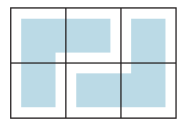
\includegraphics[scale=0.5]{../images/5.3.6.a.png}
\end{figure}
\end{proof}

\subsubsection{(b)}
Write $P(k)$.

\begin{proof}
$P(k)$ is the sentence “Any checkerboard with dimensions $2 \times 3k$ can be completely covered with L-shaped trominoes.”

\end{proof}

\subsubsection{(c)}
Write $P(k + 1)$.

\begin{proof}
$P(k + 1)$ is the sentence “Any checkerboard with dimensions $2 \times 3(k + 1)$ can be completely covered with L-shaped trominoes.”
\end{proof}

\subsubsection{(d)}
In a proof by mathematical induction that $P(n)$ is true for each integer $n \geq 1$, what must be shown in the inductive step?

\begin{proof}
The inductive step requires showing that for every integer $k \geq 1$, if any checkerboard with dimensions $2 \times 3k$ can be completely covered with L-shaped trominoes, then any checkerboard with dimensions $2 \times 3(k + 1)$ can be completely covered with L-shaped trominoes.
\end{proof}

\subsection{Exercise 7}
For each positive integer $n$, let $P(n)$ be the sentence:

In any round-robin tournament involving $n$ teams, the teams can be labeled $T_1, T_2, T_3, \ldots$, $T_n$, so that $T_i$ beats $T_{i + 1}$ for every $i = 1, 2, \ldots, n - 1$.

\subsubsection{(a)}
Write $P(2)$. Is $P(2)$ true?

\begin{proof}
$P(2)$ is the sentence ``In any round-robin tournament involving $2$ teams, the teams can be labeled $T_1, T_2$, so that $T_1$ beats $T_{2}$.'' It is true by Exercise 36 later.
\end{proof}

\subsubsection{(b)}
Write $P(k)$.

\begin{proof}
$P(k)$ is the sentence ``In any round-robin tournament involving $k$ teams, the teams can be labeled $T_1, T_2, T_3, \ldots$, $T_k$, so that $T_i$ beats $T_{i + 1}$ for every $i = 1, 2, \ldots, k$.''
\end{proof}

\subsubsection{(c)}
Write $P(k + 1)$.

\begin{proof}
$P(k + 1)$ is the sentence ``In any round-robin tournament involving $k + 1$ teams, the teams can be labeled $T_1, T_2, T_3, \ldots$, $T_{k + 1}$, so that $T_i$ beats $T_{i + 1}$ for every $i = 1, 2, \ldots, k + 1$.''
\end{proof}

\subsubsection{(d)}
In a proof by mathematical induction that $P(n)$ is true for each integer $n \geq 2$, what must be shown in the inductive step?

\begin{proof}
The inductive step requires showing that for every integer $k \geq 2$, if in any round-robin tournament involving $k$ teams, the teams can be labeled $T_1, T_2, T_3, \ldots$, $T_k$, so that $T_i$ beats $T_{i + 1}$ for every $i = 1, 2, \ldots, k$, then in any round-robin tournament involving $k + 1$ teams, the teams can be labeled $T_1, T_2, T_3, \ldots$, $T_{k + 1}$, so that $T_i$ beats $T_{i + 1}$ for every $i = 1, 2, \ldots, k + 1$.
\end{proof}

{\bf \cy Prove each statement in $8-23$ by mathematical induction.}

\subsection{Exercise 8}
$5^n - 1$ is divisible by 4, for every integer $n \geq 0$.

\begin{proof}
For the given statement, the property $P(n)$ is the sentence “$5^n - 1$ is divisible by 4.” 

{\bf Show that $P(0)$ is true:} 

$P(0)$ is the sentence “$5^0 - 1$ is divisible by 4.” Now $5^0 - 1 = 1 - 1 = 0$, and 0 is divisible by 4 because $0 = 4 \cdot 0$. Thus $P(0)$ is true. 

{\bf Show that for every integer $k \geq 0$, if $P(k)$ is true then $P(k + 1)$ is true:} 

Let $k$ be any integer with $k \geq 0$, and suppose $P(k)$ is true. That is, suppose $5^k - 1$ is divisible by 4. {\it [This is the inductive hypothesis.]} We must show that $P(k + 1)$ is true. That is, we must show that $5^{k + 1} - 1$ is divisible by 4. Now 

$5^{k + 1} - 1 = 5^k \cdot 5 - 1 = 5^k \cdot (4 + 1) - 1 = 5^k \cdot 4 + (5^k - 1)$. (*) 

By the inductive hypothesis, $5^k - 1$ is divisible by 4, and so $5^k - 1 = 4r$ for some integer $r$. Substitute $4r$ in place of $5^k - 1$ in equation (*), to obtain 

$5^{k + 1} - 1 = 5^k \cdot 4 + 4r = 4(5^k + r)$. 

But $5^k + r$ is an integer because $k$ and $r$ are integers. Hence, by definition of divisibility, $5^{k + 1} - 1$ is divisible by 4 {\it [as was to be shown]}. 

{\it An alternative proof of the inductive step goes as follows:} 

Let $k$ be any integer with $k \geq 0$, and suppose that $5^k - 1$ is divisible by 4. Then $5^k - 1 = 4r$ for some integer $r$, and hence $5^k = 4r + 1$. It follows that $5^{k + 1} = 5k \cdot 5 = (4r + 1) \cdot 5 = 20r + 5$. Subtracting 1 from both sides gives that $5^{k + 1} - 1 = 20r + 4 = 4(5r + 1)$. Now since $5r + 1$ is an integer, by definition of divisibility, $5^{k + 1} - 1$ is divisible by 4.
\end{proof}

\subsection{Exercise 9}
$7^n - 1$ is divisible by 6, for each integer $n \geq 0$.

\begin{proof}
For the given statement, the property $P(n)$ is the sentence “$7^n - 1$ is divisible by 6.” 

{\bf Show that $P(0)$ is true:} 

$P(0)$ is the sentence “$7^0 - 1$ is divisible by 6.” Now $7^0 - 1 = 1 - 1 = 0$, and 0 is divisible by 6 because $0 = 6 \cdot 0$. Thus $P(0)$ is true. 

{\bf Show that for every integer $k \geq 0$, if $P(k)$ is true then $P(k + 1)$ is true:} 

Let $k$ be any integer with $k \geq 0$, and suppose $P(k)$ is true. That is, suppose $7^k - 1$ is divisible by 6. {\it [This is the inductive hypothesis.]} We must show that $P(k + 1)$ is true. That is, we must show that $7^{k + 1} - 1$ is divisible by 6. Now 

$7^{k + 1} - 1 = 7^k \cdot 7 - 1 = 7^k \cdot (6 + 1) - 1 = 7^k \cdot 6 + (7^k - 1)$. (*) 

By the inductive hypothesis, $7^k - 1$ is divisible by 6, and so $7^k - 1 = 6r$ for some integer $r$. Substitute $6r$ in place of $7^k - 1$ in equation (*), to obtain 

$7^{k + 1} - 1 = 7^k \cdot 6 + 6r = 6(7^k + r)$. 

But $7^k + r$ is an integer because $k$ and $r$ are integers. Hence, by definition of divisibility, $7^{k + 1} - 1$ is divisible by 6 {\it [as was to be shown]}.
\end{proof}

\subsection{Exercise 10}
$n^3 - 7n + 3$ is divisible by 3, for each integer $n \geq 0$.

\begin{proof}
For the given statement, the property $P(n)$ is the sentence “$n^3 - 7n + 3$ is divisible by 3.” 

{\bf Show that $P(0)$ is true:} 

$P(0)$ is the sentence “$0^3 - 7 \cdot 0 + 3$ is divisible by 3.” Now $0^3 - 7 \cdot 0 + 3 = 3$, and 3 is divisible by 3 because $3 = 1 \cdot 3$. Thus $P(0)$ is true. 

{\bf Show that for every integer $k \geq 0$, if $P(k)$ is true then $P(k + 1)$ is true:} 

Let $k$ be any integer with $k \geq 0$, and suppose $P(k)$ is true. That is, suppose $k^3 - 7k + 3$ is divisible by 3. {\it [This is the inductive hypothesis.]} We must show that $P(k + 1)$ is true. That is, we must show that $(k+1)^3 - 7(k+1) + 3$ is divisible by 3. Now 

$(k+1)^3 - 7(k+1) + 3 = k^3 + 3k^2 + 3k + 1 - 7k - 7 + 3 = (k^3 - 7k + 3) + 3(k^2 + k - 2)$. (*) 

By the inductive hypothesis, $k^3 - 7k + 3$ is divisible by 3, and so $k^3 - 7k + 3 = 3r$ for some integer $r$. Substitute $3r$ in place of $k^3 - 7k + 3$ in equation (*), to obtain 

$(k+1)^3 - 7(k+1) + 3 = 3r + 3(k^2 + k - 2) = 3(r + k^2 + k - 2)$. 

But $r + k^2 + k - 2$ is an integer because $k$ and $r$ are integers. Hence, by definition of divisibility, $(k+1)^3 - 7(k+1) + 3$ is divisible by 3 {\it [as was to be shown]}.
\end{proof}

\subsection{Exercise 11}
$3^{2n} - 1$ is divisible by 8, for each integer $n \geq 0$.

\begin{proof}
For the given statement, the property $P(n)$ is the sentence “$3^{2n} - 1$ is divisible by 8.” 

{\bf Show that $P(0)$ is true:} 

$P(0)$ is the sentence “$3^{2 \cdot 0} - 1$ is divisible by 8.” Now $3^{2 \cdot 0} - 1 = 1 - 1 = 0$, and 0 is divisible by 8 because $0 = 8 \cdot 0$. Thus $P(0)$ is true. 

{\bf Show that for every integer $k \geq 0$, if $P(k)$ is true then $P(k + 1)$ is true:} 

Let $k$ be any integer with $k \geq 0$, and suppose $P(k)$ is true. That is, suppose $3^{2k} - 1$ is divisible by 8. {\it [This is the inductive hypothesis.]} We must show that $P(k + 1)$ is true. That is, we must show that $3^{2(k+1)} - 1$ is divisible by 8. Now 

$3^{2(k+1)} - 1 = 3^{2k+2} - 1 = 3^{2k} \cdot 3^2 - 1 = 3^{2k} \cdot 9 - 1 = 3^{2k} \cdot (8+1) - 1 = 3^{2k} \cdot 8 + 3^{2k} - 1$. (*) 

By the inductive hypothesis, $3^{2k} - 1$ is divisible by 8, and so $3^{2k} - 1 = 8r$ for some integer $r$. Substitute $8r$ in place of $3^{2k} - 1$ in equation (*), to obtain 

$3^{2(k+1)} - 1 = 3^{2k} \cdot 8 + 8r = 8(3^{2k} + r)$. 

But $3^{2k} + r$ is an integer because $k$ and $r$ are integers. Hence, by definition of divisibility, $3^{2(k+1)} - 1$ is divisible by 8 {\it [as was to be shown]}.
\end{proof}

\subsection{Exercise 12}
For any integer $n \geq 0$, $7^n - 2^n$ is divisible by 5.

\begin{proof}
For the given statement, the property $P(n)$ is the sentence “$7^n - 2^n$ is divisible by 5.” 

{\bf Show that $P(0)$ is true:} 

$P(0)$ is the sentence “$7^0 - 2^0$ is divisible by 5.” Now $7^0 - 2^0 = 1 - 1 = 0$, and 0 is divisible by 5 because $0 = 5 \cdot 0$. Thus $P(0)$ is true. 

{\bf Show that for every integer $k \geq 0$, if $P(k)$ is true then $P(k + 1)$ is true:} 

Let $k$ be any integer with $k \geq 0$, and suppose $P(k)$ is true. That is, suppose $7^k - 2^k$ is divisible by 5. {\it [This is the inductive hypothesis.]} We must show that $P(k + 1)$ is true. That is, we must show that $7^{k+1} - 2^{k+1}$ is divisible by 5. Now 

$7^{k+1} - 2^{k+1} = 7 \cdot 7^k - 2 \cdot 2^k = (5+2) \cdot 7^k - 2 \cdot 2^k = 5 \cdot 7^k + 2(7^k - 2^k)$. (*) 

By the inductive hypothesis, $7^k - 2^k$ is divisible by 5, and so $7^k - 2^k = 5r$ for some integer $r$. Substitute $5r$ in place of $7^k - 2^k$ in equation (*), to obtain 

$7^{k+1} - 2^{k+1} = 5 \cdot 7^k + 2(5r) = 5(7^k + 2r)$. 

But $7^k + 2r$ is an integer because $k$ and $r$ are integers. Hence, by definition of divisibility, $7^{k+1} - 2^{k+1}$ is divisible by 5 {\it [as was to be shown]}.
\end{proof}

\subsection{Exercise 13}
For any integer $n \geq 0, x^n - y^n$ is divisible by $x - y$, where $x$ and $y$ are any integers with $x \neq y$.

{\it Hint:} $x^{k+1} - y^{k+1} = x^{k+1} - xy^k + xy^k - y^{k+1} = x(x^k - y^k) + y^k(x-y)$.

\begin{proof}
For the given statement, the property $P(n)$ is the sentence “$x^n - y^n$ is divisible by $x - y$.” 

{\bf Show that $P(0)$ is true:} 

$P(0)$ is the sentence “$x^0 - y^0$ is divisible by $x - y$..” Now $x^0 - y^0 = 1 - 1 = 0$, and 0 is divisible by $x - y$ because $0 = (x-y) \cdot 0$. Thus $P(0)$ is true. 

{\bf Show that for every integer $k \geq 0$, if $P(k)$ is true then $P(k + 1)$ is true:} 

Let $k$ be any integer with $k \geq 0$, and suppose $P(k)$ is true. That is, suppose $x^k - y^k$ is divisible by $x-y$. {\it [This is the inductive hypothesis.]} We must show that $P(k + 1)$ is true. That is, we must show that $7^{k+1} - 2^{k+1}$ is divisible by $x-y$. Now 

$x^{k+1} - y^{k+1} = x^{k+1} - xy^k + xy^k - y^{k+1} = x(x^k - y^k) + y^k(x-y)$. (*) 

By the inductive hypothesis, $x^k - y^k$ is divisible by $x-y$, and so $x^k - y^k = (x-y)r$ for some integer $r$. Substitute $(x-y)r$ in place of $x^k - y^k$ in equation (*), to obtain 

$x^{k+1} - y^{k+1} = x(x - y)r + y^k(x-y) = (x-y)[xr + y^k]$. 

But $xr + y^k$ is an integer because $k, x, y$ and $r$ are integers. Hence, by definition of divisibility, $x^{k+1} - y^{k+1}$ is divisible by $x - y$ {\it [as was to be shown]}.
\end{proof}

\subsection{Exercise 14}
$n^3 - n$ is divisible by 6, for each integer $n \geq 0$.

{\it Hint 1:} $(k + 1)^3 - (k + 1) = k^3 + 3k^2 + 3k + 1 - k - 1 = (k^3 - k) + 3k^2 + 3k = (k^3 - k) + 3k(k + 1)$.

{\it Hint 2:} $k(k + 1)$ is a product of two consecutive integers. By Theorem 4.5.2, one of these must be even.

\begin{proof}
{\it Note:} It is possible to prove this without mathematical induction, because $n^3 - n = n(n^2 - 1) = n(n-1)(n+1)$ is the product of 3 consecutive integers. Therefore one of them is divisible by 3, and one of them is even, hence their product is divisible by 6.

For the given statement, the property $P(n)$ is the sentence “$n^3 - n$ is divisible by 6.” 

{\bf Show that $P(0)$ is true:} 

$P(0)$ is the sentence “$n^3 - n$ is divisible by 6.” Now $0^3 - 0 = 0 - 0 = 0$, and 0 is divisible by 6 because $0 = 6 \cdot 0$. Thus $P(0)$ is true. 

{\bf Show that for every integer $k \geq 0$, if $P(k)$ is true then $P(k + 1)$ is true:} 

Let $k$ be any integer with $k \geq 0$, and suppose $P(k)$ is true. That is, suppose $k^3 - k$ is divisible by 6. {\it [This is the inductive hypothesis.]} We must show that $P(k + 1)$ is true. That is, we must show that $(k+1)^3 - (k+1)$ is divisible by 6. Now 

$(k + 1)^3 - (k + 1) = k^3 + 3k^2 + 3k + 1 - k - 1 = (k^3 - k) + 3k(k + 1)$. (*)

By the inductive hypothesis, $k^3 - k$ is divisible by 6, and so $k^3 - k = 6r$ for some integer $r$. Moreover $k(k+1)$ is even by Theorem 4.5.2, so $k(k+1) = 2s$ for some integer $s$. Substitute $6r$ in place of $k^3 - k$ and $2s$ in place of $k(k+1)$ in equation (*), to obtain 

$(k + 1)^3 - (k + 1) = 6r + 3(2s) = 6r + 6s = 6(r+s)$.

But $r+s$ is an integer because $r$ and $s$ are integers. Hence, by definition of divisibility, $(k + 1)^3 - (k + 1)$ is divisible by 6 {\it [as was to be shown]}.
\end{proof}

\subsection{Exercise 15}
$n(n^2 + 5)$ is divisible by 6, for each integer $n \geq 0$.

\begin{proof}
For the given statement, the property $P(n)$ is the sentence “$n(n^2 + 5)$ is divisible by 6.” 

{\bf Show that $P(0)$ is true:} 

$P(0)$ is the sentence “$0(0^2 + 5)$ is divisible by 6.” Now $0(0^2 + 5) = 0$, and 0 is divisible by 6 because $0 = 6 \cdot 0$. Thus $P(0)$ is true. 

{\bf Show that for every integer $k \geq 0$, if $P(k)$ is true then $P(k + 1)$ is true:} 

Let $k$ be any integer with $k \geq 0$, and suppose $P(k)$ is true. That is, suppose $k(k^2 + 5)$ is divisible by 6. {\it [This is the inductive hypothesis.]} We must show that $P(k + 1)$ is true. That is, we must show that $(k+1)((k+1)^2 + 5)$ is divisible by 6. Now 

$(k+1)((k+1)^2 + 5) = (k+1)^3 + 5(k+1) = k^3 + 3k^2 + 3k + 1 + 5k + 5 =$

$= (k^3 + 5k) + (3k^2 + 3k + 6) = k(k^2 + 5) + 3(k^2 + k + 2) = k(k^2 + 5) + 3(k(k+1) + 2)$. (*)

By the inductive hypothesis, $k(k^2 + 5)$ is divisible by 6, and so $k(k^2 + 5) = 6r$ for some integer $r$. Moreover $k(k+1)$ is even by Theorem 4.5.2, so $k(k+1) = 2s$ for some integer $s$. Substitute $6r$ in place of $k(k^2 + 5)$ and $2s$ in place of $k(k+1)$ in equation (*), to obtain 

$(k+1)((k+1)^2 + 5) = 6r + 3(2s + 2) = 6r + 6s + 6 = 6(r + s + 1)$.

But $r + s + 1$ is an integer because $r$ and $s$ are integers. Hence, by definition of divisibility, $(k + 1)((k + 1)^2 + 5)$ is divisible by 6 {\it [as was to be shown]}.
\end{proof}

\subsection{Exercise 16}
$2^n < (n + 1)!$, for every integer $n \geq 2$.

\begin{proof}
For the given statement, the property $P(n)$ is the inequality $2^n < (n + 1)!$. 

{\bf Show that $P(2)$ is true:} 

$P(2)$ says that $2^2 < (2 + 1)!$. The left-hand side is $2^2 = 4$ and the right-hand side is $(2+1)! = 3! = 6$. So, because $4 < 6$, $P(2)$ is true. 

{\bf Show that for every integer $k \geq 2$, if $P(k)$ is true then $P(k + 1)$ is true:} 

Let $k$ be any integer with $k \geq 2$, and suppose $P(k)$ is true. That is, suppose $2^k < (k + 1)!$. {\it [This is the inductive hypothesis.]} We must show that $P(k + 1)$ is true. That is, we must show that $2^{k+1} < ((k+1) + 1)!$, or, equivalently, $2^{k+1} < (k + 2)!$. By the laws of exponents and the induction hypothesis,
\[
2^{k+1} = 2 \cdot 2^k < 2(k+1)!.
\]
Since $k \geq 2$, then $2 < k+2$, so
\[
2^{k+1} = 2 \cdot 2^k < 2(k+1)! < (k+2)(k+1)! = (k+2)!.
\]
So $2^{k+1} < (k+2)!$ {\it [as was to be shown]}.
\end{proof}

\subsection{Exercise 17}
$1 + 3n \leq 4^n$, for every integer $n \geq 0$.

\begin{proof}
For the given statement, the property $P(n)$ is the inequality $1 + 3n \leq 4^n$. 

{\bf Show that $P(0)$ is true:} 

$P(0)$ says that $1 + 3 \cdot 0 \leq 4^0$. The left-hand side is $1 + 3 \cdot 0 = 1$ and the right-hand side is $4^0 = 1$. So, because $1 \leq 1$, $P(0)$ is true. 

{\bf Show that for every integer $k \geq 0$, if $P(k)$ is true then $P(k + 1)$ is true:} 

Let $k$ be any integer with $k \geq 0$, and suppose $P(k)$ is true. That is, suppose $1 + 3k \leq 4^k$. {\it [This is the inductive hypothesis.]} We must show that $P(k + 1)$ is true. That is, we must show that $1 + 3(k+1) \leq 4^{k+1}$, or, equivalently, $1+3k+3 < 4 \cdot 4^k$. 

Now by the induction hypothesis, $1 + 3k + 3 \leq 4^k + 3$. So we need to show that $4^k + 3 \leq 4 \cdot 4^k$.

Since $0 \leq k$, we have $1 \leq 4^k$. So $3 \leq 3 \cdot 4^k$. Adding $4^k$ to both sides we get $3 + 4^k \leq 3 \cdot 4^k + 4^k = 4 \cdot 4^k$. Thus $3 + 4^k \leq 4 \cdot 4^k$.

So we have $1 + 3k + 3 \leq 4^k + 3$ and $3 + 4^k \leq 4 \cdot 4^k$. Combining these we get $1 + 3k + 3 \leq 4 \cdot 4^k$, in other words $1 + 3(k+1) \leq 4^{k+1}$, {\it [as was to be shown]}.
\end{proof}

\subsection{Exercise 18}
$5^n + 9 < 6^n$, for each integer $n \geq 2$.

\begin{proof}
For the given statement, the property $P(n)$ is the inequality $5^n + 9 < 6^n$. 

{\bf Show that $P(2)$ is true:} 

$P(2)$ says that $5^2 + 9 < 6^2$. The left-hand side is $5^2 + 9 = 25 + 9 = 34$ and the right-hand side is $6^2 = 36$. So, because $34 < 36$, $P(2)$ is true. 

{\bf Show that for every integer $k \geq 2$, if $P(k)$ is true then $P(k + 1)$ is true:} 

Let $k$ be any integer with $k \geq 2$, and suppose $P(k)$ is true. That is, suppose $5^k + 9 < 6^k$. {\it [This is the inductive hypothesis.]} We must show that $P(k + 1)$ is true. That is, we must show that $5^{k+1} + 9 < 6^{k+1}$. Now by laws of exponents and the induction hypothesis,
\[
5^{k+1} + 9 = 5 \cdot 5^k + 9 = (4 + 1) \cdot 5^k + 9 = 4 \cdot 5^k + (5^k + 9) < 4 \cdot 5^k + 6^k. (*)
\]
So we need to show $4 \cdot 5^k + 6^k < 6^{k+1}$.

Notice that since $4 < 5$ (and $5^k$ is positive) we have $4 \cdot 5^k < 5 \cdot 5^k$, and since $5 < 6$ (and $k \geq 2$) we have $5^k < 6^k$, and therefore $5 \cdot 5^k < 5 \cdot 6^k$. By transitivity of $<$, we get $4 \cdot 5^k < 5 \cdot 6^k$.

Since $4 \cdot 5^k < 5 \cdot 6^k$, adding $6^k$ to both sides we get $4 \cdot 5^k + 6^k < 5 \cdot 6^k + 6^k = 6 \cdot 6^k = 6^{k+1}$.

Combining this with (*) we get $5^{k+1} + 9 < 6^{k+1}$, {\it [as was to be shown]}.
\end{proof}

\subsection{Exercise 19}
$n^2 < 2^n$, for every integer $n \geq 5$.

\begin{proof}
For the given statement, the property $P(n)$ is the inequality $n^2 < 2^n$. 

{\bf Show that $P(5)$ is true:} 

$P(5)$ says that $5^2 < 2^5$. The left-hand side is $5^2 = 25$ and the right-hand side is $2^5 = 32$. So, because $25 < 32$, $P(5)$ is true. 

{\bf Show that for every integer $k \geq 5$, if $P(k)$ is true then $P(k + 1)$ is true:} 

Let $k$ be any integer with $k \geq 5$, and suppose $P(k)$ is true. That is, suppose $k^2 < 2^k$. {\it [This is the inductive hypothesis.]} We must show that $P(k + 1)$ is true. That is, we must show that $(k+1)^2 < 2^{k+1}$. 

Now by algebra and the induction hypothesis, $(k+1)^2 = k^2 + 2k + 1 < 2^k + 2k + 1$. Also by Proposition 5.3.2, $2k + 1 < 2^k$. Putting these inequalities together gives
\[
(k+1)^2 < 2^k + 2k + 1 < 2^k + 2^k = 2 \cdot 2^k = 2^{k+1}
\]
{\it [as was to be shown]}.
\end{proof}

\subsection{Exercise 20}
$2^n < (n + 2)!$, for each integer $n \geq 0$.

\begin{proof}
For the given statement, the property $P(n)$ is the inequality $n^2 < 2^n$. 

{\bf Show that $P(0)$ is true:} 

$P(0)$ says that $2^0 < (0 + 2)!$. The left-hand side is $2^0 = 1$ and the right-hand side is $(0 + 2)! = 2! = 2$. So, because $1 < 2$, $P(0)$ is true. 

{\bf Show that for every integer $k \geq 0$, if $P(k)$ is true then $P(k + 1)$ is true:} 

Let $k$ be any integer with $k \geq 0$, and suppose $P(k)$ is true. That is, suppose $2^k < (k + 2)!$. {\it [This is the inductive hypothesis.]} We must show that $P(k + 1)$ is true. That is, we must show that $2^{k+1} < (k + 3)!$. 

Now $2^{k+1} = 2 \cdot 2^k < 2 \cdot (k+2)!$ by the induction hypothesis. Since $k \geq 0$, we have $2 < k+3$, so $2 \cdot (k+2)! < (k+3) \cdot (k+2)! = (k+3)!$. Putting these two inequalities together gives $2^{k+1} < (k+3)!$, {\it [as was to be shown]}.
\end{proof}

\subsection{Exercise 21}
$\dps \sqrt{n} < \frac{1}{\sqrt{1}} + \frac{1}{\sqrt{2}} + \cdots + \frac{1}{\sqrt{n}}$, for every integer $n \geq 2$.

\begin{proof}
For the given statement, the property $P(n)$ is the inequality $\dps \sqrt{n} < \frac{1}{\sqrt{1}} + \frac{1}{\sqrt{2}} + \cdots + \frac{1}{\sqrt{n}}$. 

{\bf Show that $P(2)$ is true:} 

$P(2)$ says that $\dps \sqrt{2} < \frac{1}{\sqrt{1}} + \frac{1}{\sqrt{2}}$. The left-hand side is $\dps \sqrt{2} \approx 1.414$ and the right-hand side is $\dps \frac{1}{\sqrt{1}} + \frac{1}{\sqrt{2}} \approx 1 + \frac{1}{1.414} = 1.707$. So, because $1.414 < 1.707$, $P(2)$ is true. 

{\bf Show that for every integer $k \geq 2$, if $P(k)$ is true then $P(k + 1)$ is true:} 

Let $k$ be any integer with $k \geq 2$, and suppose $P(k)$ is true. That is, suppose $\dps \sqrt{k} < \frac{1}{\sqrt{1}} + \frac{1}{\sqrt{2}} + \cdots + \frac{1}{\sqrt{k}}$. {\it [This is the inductive hypothesis.]} We must show that $P(k + 1)$ is true. That is, we must show that $\dps \sqrt{k+1} < \frac{1}{\sqrt{1}} + \frac{1}{\sqrt{2}} + \cdots + \frac{1}{\sqrt{k+1}}$. 

Now the right-hand side of $P(k+1)$ is $\dps \frac{1}{\sqrt{1}} + \frac{1}{\sqrt{2}} + \cdots + \frac{1}{\sqrt{k+1}}$

\begin{center}
\begin{tabular}{lll}
= & $\dps \frac{1}{\sqrt{1}} + \frac{1}{\sqrt{2}} + \cdots + \frac{1}{\sqrt{k}} + \frac{1}{\sqrt{k+1}}$ & {\cy make next-to-last term explicit} \\
$>$ & $\dps \sqrt{k} + \frac{1}{\sqrt{k+1}}$ & {\cy by inductive hypothesis} \\
= & $\dps \sqrt{k} \cdot \frac{\sqrt{k + 1}}{\sqrt{k + 1}} + \frac{1}{\sqrt{k+1}}$ & {\cy because $\frac{\sqrt{k + 1}}{\sqrt{k + 1}} = 1$} \\
$>$ & $\dps \sqrt{k} \cdot \frac{\sqrt{k}}{\sqrt{k + 1}} + \frac{1}{\sqrt{k+1}}$ & {\cy because $k + 1 > k$} \\
= & $\dps \frac{k}{\sqrt{k + 1}} + \frac{1}{\sqrt{k+1}}$ & {\cy by algebra} \\
= & $\dps \frac{k+1}{\sqrt{k + 1}}$ & {\cy by adding fractions} \\
= & $\dps \sqrt{k + 1}$ & {\cy by canceling $\sqrt{k+1}$}
\end{tabular}
\end{center}

{\it [as was to be shown]}.
\end{proof}

\subsection{Exercise 22}
$1 + nx \leq (1 + x)^n$, for every real number $x > -1$
and every integer $n \geq 2$.

\begin{proof}
For the given statement, the property $P(n)$ is the statement ``$1 + nx \leq (1 + x)^n$, for every real number $x > -1$''. 

{\bf Show that $P(2)$ is true:} 

$P(2)$ says that $1 + 2x \leq (1 + x)^2$, for every real number $x > -1$. The left-hand side is $1 + 2x$ and the right-hand side is $(1+x)^2 = 1 + 2x + x^2$. So, because $0 \leq x^2$ for every real number $x > -1$, adding $1 + 2x$ to both sides gives us $1 + 2x \leq 1 + 2x + x^2$. So $P(2)$ is true. 

{\bf Show that for every integer $k \geq 2$, if $P(k)$ is true then $P(k + 1)$ is true:} 

Let $k$ be any integer with $k \geq 2$, and suppose $P(k)$ is true. That is, suppose $1 + kx \leq (1 + x)^k$, for every real number $x > -1$. {\it [This is the inductive hypothesis.]} We must show that $P(k + 1)$ is true. That is, we must show that $1 + (k + 1)x \leq (1 + x)^{k + 1}$, for every real number $x > -1$. 

Now the left-hand side of $P(k+1)$ is $1 + (k + 1)x = 1 + kx + x \leq (1 + x)^k + x$ by inductive hypothesis. 

We want to show $x \leq x(1+x)^k$. There are two cases:

{\bf Case 1: $-1 < x < 0$.} Then $0 < 1 + x < 1$, so $0 < (1+x)^k < 1$. So $0 > x(1+x)^k > x$ (since $x$ is negative).

{\bf Case 2: $0 \leq x$.} Then $1 \leq 1+x$, so $1 \leq (1 + x)^k$. Multiplying both sides by $x$ we get $x \leq x(1 + x)^k$ since $x$ is positive.

Combining the two inequalities $1 + (k + 1)x \leq (1 + x)^k + x$ and $x \leq x(1 + x)^k$ we get 
\[
1 + (k + 1)x \leq (1 + x)^k + x(1 + x)^k = (1 + x)^k (1 + x) = (1 + x)^{k + 1}
\]
{\it [as was to be shown]}.
\end{proof}

\subsection{Exercise 23}

\subsubsection{(a)}
$n^3 > 2n + 1$, for each integer $n \geq 2$.

\begin{proof}
For the given statement, the property $P(n)$ is the inequality $n^3 > 2n + 1$. 

{\bf Show that $P(2)$ is true:} 

$P(2)$ says that $2^3 > 2\cdot2 + 1$. The left-hand side is $2^3 = 8$ and the right-hand side is $2 \cdot 2 + 1 = 5$. So, because $8 > 5$, $P(2)$ is true. 

{\bf Show that for every integer $k \geq 2$, if $P(k)$ is true then $P(k + 1)$ is true:} 

Let $k$ be any integer with $k \geq 2$, and suppose $P(k)$ is true. That is, suppose $k^3 > 2k + 1$. {\it [This is the inductive hypothesis.]} We must show that $P(k + 1)$ is true. That is, we must show that $(k + 1)^3 > 2(k + 1) + 1$. 

Now $(k + 1)^3 = k^3 + 3k^2 + 3k + 1 > (2k + 1) + 3k^2 + 3k + 1$ by the induction hypothesis. Since $k \geq 2$, we have $3k^2 + 3k \geq 3 \cdot 2^2 + 3 \cdot 2 = 18 > 2$, so
\[
(k + 1)^3 > (2k + 1) + 3k^2 + 3k + 1 > 2k + 1 + 2 = 2k + 3 = 2(k + 1) + 1
\]
{\it [as was to be shown]}.
\end{proof}

\subsubsection{(b)}
$n! > n^2$, for each integer $n \geq 4$.

\begin{proof}
For the given statement, the property $P(n)$ is the inequality $n! > n^2$. 

{\bf Show that $P(4)$ is true:} 

$P(4)$ says that $4! > 4^2$. The left-hand side is $4! = 24$ and the right-hand side is $4^2 = 16$. So, because $24 > 16$, $P(4)$ is true. 

{\bf Show that for every integer $k \geq 4$, if $P(k)$ is true then $P(k + 1)$ is true:} 

Let $k$ be any integer with $k \geq 4$, and suppose $P(k)$ is true. That is, suppose $k! > k^2$. {\it [This is the inductive hypothesis.]} We must show that $P(k + 1)$ is true. That is, we must show that $(k + 1)! > (k + 1)^2$. 

We have $(k + 1)! = (k + 1) \cdot k! > (k + 1) \cdot k^2$ by the induction hypothesis. So we need to show $(k + 1) \cdot k^2 > (k + 1)^2$, or, equivalently, $k^2 > k+1$, or equivalently $k^2 - k - 1 > 0$.

From analytic geometry, we know that the roots of the equation $k^2 - k - 1 = 0$ are $k = \dps \frac{-(-1) \pm \sqrt{(-1)^2 - 4(1)(-1)}}{2(1)} = \frac{1 \pm \sqrt{5}}{2} \approx 0.618$ and $1.618$. Since the leading coefficient of the quadratic polynomial $k^2 - k - 1$ is positive, it has a U-shape and it's positive for all values of $k$ greater than the larger root 1.618. Since $k \geq 4$ it follows that $k^2 - k - 1 > 0$.
\end{proof}

\subsection{Exercise 24}
A sequence $a_1, a_2, a_3, \ldots$ is defined by letting $a_1 = 3$ and $a_k = 7a_{k-1}$ for each integer $k \geq 2$. Show that $a_n = 3\cdot 7^n - 1$ for every integer $n \geq 1$.

\begin{proof}
For the given statement, the property $P(n)$ is the equation $a_n = 3 \cdot 7^{n - 1}$. 

{\bf Show that $P(1)$ is true:} 

The left-hand side is $a_1$, which equals 3 by the definition of the sequence. The right-hand side is $4 \cdot 7^{1 - 1} = 3$ also. Thus $P(1)$ is true. 

{\bf Show that for every integer $k \geq 1$, if $P(k)$ is true then $P(k + 1)$ is true:} 

Let $k$ be any integer with $k \geq 1$, and suppose $P(k)$ is true. That is, suppose $a_k = 3 \cdot 7^{k - 1}$. {\it [This is the inductive hypothesis.]} We must show that $P(k + 1)$ is true. That is, we must show that $a_{k + 1} = 3 \cdot 7^{(k + 1) - 1}$, or, equivalently, $a_{k + 1} = 3 \cdot 7^k$. But the left-hand side of $P(k+1)$ is $a_{k+1}$

\begin{center}
\begin{tabular}{rlll}
$a_{k+1}$ & = & $7a_k$ & {\cy by definition of the sequence} \\
& = & $7(3 \cdot 7^{k - 1})$ & {\cy by inductive hypothesis} \\
& = & $3 \cdot 7^k$ & {\cy by laws of exponents} \\
\end{tabular}
\end{center}

which is the right-hand side of $P(k + 1)$, {\it [as was to be shown]}.
\end{proof}

\subsection{Exercise 25}
A sequence $b_0, b_1, b_2, \ldots$ is defined by letting
$b_0 = 5$ and $b_k = 4 + b_{k-1}$ for each integer $k \geq 1$. Show that $b_n > 4n$ for every integer $n \geq 0$.

\begin{proof}
Let the property $P(n)$ be the inequality $b_n > 4n$. 

{\bf Show that $P(0)$ is true:} 

The left-hand side is $b_0$, which equals 5 by the definition of the sequence. The right-hand side is $4 \cdot 0 = 0$ and $5 > 0$. Thus $P(0)$ is true. 

{\bf Show that for every integer $k \geq 0$, if $P(k)$ is true then $P(k + 1)$ is true:} 

Let $k$ be any integer with $k \geq 0$, and suppose that $b_k > 4k$ ({\cy inductive hypothesis}). We must show that $b_{k + 1} > 4(k+1)$. Now

\begin{center}
\begin{tabular}{rlll}
$b_{k+1}$ & = & $4 + b_k$ & {\cy by definition of the sequence} \\
& $>$ & $4 + 4k$ & {\cy by inductive hypothesis} \\
& = & $4(1 + k)$ & {\cy by factoring out a 4} \\
& = & $4(k + 1)$ & {\cy by commutative law for addition}
\end{tabular}
\end{center}

{\it [as was to be shown]}.
\end{proof}

\subsection{Exercise 26}
A sequence $c_0, c_1, c_2, \ldots$ is defined by letting
$c_0 = 3$ and $c_k = (c_{k-1})^2$ for every integer $k \geq 1$. Show that $\dps c_n = 3^{2^n}$ for each integer $n \geq 0$.

\begin{proof}
Let the property $P(n)$ be the equation $\dps c_n = 3^{2^n}$. 

{\bf Show that $P(0)$ is true:} 

The left-hand side is $c_0$, which equals 3 by the definition of the sequence. The right-hand side is $\dps 3^{2^0} = 3^1 = 3$ and $3 = 3$. Thus $P(0)$ is true. 

{\bf Show that for every integer $k \geq 0$, if $P(k)$ is true then $P(k + 1)$ is true:} 

Let $k$ be any integer with $k \geq 0$, and suppose that $\dps c_k = 3^{2^k}$ ({\cy inductive hypothesis}). We must show that $c_{k + 1} = 3^{2^{k+1}}$. Now

\begin{center}
\begin{tabular}{rlll}
$c_{k+1}$ & = & $(c_k)^2$ & {\cy by definition of the sequence} \\
& = & $\dps (3^{2^k})^2$ & {\cy by inductive hypothesis} \\
& = & $3^{2^k \cdot 2}$ & {\cy by laws of exponents} \\
& = & $3^{2^{k + 1}}$ & {\cy by laws of exponents}
\end{tabular}
\end{center}

{\it [as was to be shown]}.
\end{proof}

\subsection{Exercise 27}
A sequence $d_1, d_2, d_3, \ldots$ is defined by letting $d_1 = 2$ and $\dps d_k = \frac{d_{k-1}}{k}$ for each integer $k \geq 2$. Show that for every integer $\dps n \geq 1, d_n = \frac{2}{n!}$. 

\begin{proof}
Let the property $P(n)$ be the equation $\dps d_n = \frac{2}{n!}$. 

{\bf Show that $P(1)$ is true:} 

The left-hand side is $d_1$, which equals 2 by the definition of the sequence. The right-hand side is $\dps \frac{2}{1!} = 2$ and $2 = 2$. Thus $P(1)$ is true. 

{\bf Show that for every integer $k \geq 1$, if $P(k)$ is true then $P(k + 1)$ is true:} 

Let $k$ be any integer with $k \geq 1$, and suppose that $\dps d_k = \frac{2}{k!}$ ({\cy inductive hypothesis}). We must show that $\dps d_{k + 1} = \frac{2}{(k + 1)!}$. Now

\begin{center}
\begin{tabular}{rlll}
\vspace{0.3cm}
$d_{k+1}$ & = & $\dps \frac{d_k}{k+1}$ & {\cy by definition of the sequence} \\
\vspace{0.3cm}
& = & $\dps \frac{\frac{2}{k!}}{k+1}$ & {\cy by inductive hypothesis} \\
& = & $\dps \frac{2}{k!(k+1)}$ & {\cy by algebra} \\
& = & $\dps \frac{2}{(k + 1)!}$ & {\cy by definition of !}
\end{tabular}
\end{center}

{\it [as was to be shown]}.
\end{proof}

\subsection{Exercise 28}
Prove that for every integer $n \geq 1$,
\[
\frac{1}{3} = \frac{1 + 3 + 5 + \cdots + (2n-1)}{(2n+1) + (2n+3) + \cdots + (2n + (2n-1))}
\]
\begin{proof}
Let the property $P(n)$ be the equation 

\[
\dps \frac{1}{3} = \frac{1 + 3 + 5 + \cdots + (2n-1)}{(2n+1) + (2n+3) + \cdots + (2n + (2n-1))}.
\] 

{\bf Show that $P(1)$ is true:} 

The left-hand side is $1/3$. The right-hand side is $\dps \frac{1}{(2 \cdot 1 + 1)} = 1/3$ also. Thus $P(1)$ is true. 

{\bf Show that for every integer $k \geq 1$, if $P(k)$ is true then $P(k + 1)$ is true:} 

Let $k$ be any integer with $k \geq 1$, and suppose that 
\[
\dps \frac{1}{3} = \frac{1 + 3 + 5 + \cdots + (2k-1)}{(2k+1) + (2k+3) + \cdots + (2k + (2k-1))}
\]
({\cy inductive hypothesis}). We must show that 
\[
\dps \frac{1}{3} = \frac{1 + 3 + 5 + \cdots + (2(k+1)-1)}{(2(k+1)+1) + (2(k+1)+3) + \cdots + (2(k+1) + (2(k+1)-1))}.\] 
Now from the inductive hypothesis, we get by cross-multiplying:
\[
(2k+1) + (2k+3) + \cdots + (2k + (2k-1)) = 3[1 + 3 + 5 + \cdots + (2k-1)]
\]
For each term on the left-hand side, we add 2 to both sides. This way, $(2k + 1)$ becomes $(2k + 1) + 2 = (2(k+1) + 1)$, $(2k + 3)$ becomes $(2k + 3) + 2 = (2(k+1) + 3)$, and so on. There are $(2k - 1 + 1) / 2 = k$ terms on the left-hand side, therefore we are adding a total of $2k$ to both sides. We get:
\[
(2(k+1)+1) + (2(k+1)+3) + \cdots + (2(k+1) + (2k-1)) = 3[1 + 3 + 5 + \cdots + (2k-1)] + 2k
\]
Now add the last missing term $(2(k+1) + (2(k+1)-1))$ to both sides:

$(2(k+1)+1) + (2(k+1)+3) + \cdots + (2(k+1) + (2k-1)) + (2(k+1) + (2(k+1)-1))$

$ = 3[1 + 3 + 5 + \cdots + (2k-1)] + 2k + (2(k+1) + (2(k+1)-1))$

Notice that $2k + (2(k+1) + (2(k+1)-1)) = 6k + 3 = 3(2k+1) = 3(2(k+1) - 1)$. Therefore

$(2(k+1)+1) + (2(k+1)+3) + \cdots + (2(k+1) + (2k-1)) + (2(k+1) + (2(k+1)-1))$

$ = 3[1 + 3 + 5 + \cdots + (2k-1) + (2(k+1)-1)]$.

Dividing both sides by (3 times the left-hand side), we get:
\[
\dps \frac{1}{3} = \frac{1 + 3 + 5 + \cdots + (2(k+1)-1)}{(2(k+1)+1) + (2(k+1)+3) + \cdots + (2(k+1) + (2(k+1)-1))}\] 
{\it [as was to be shown]}.
\end{proof}

{\bf \cy Exercises 29 and 30 use the definition of string and string length from page 13 in Section 1.4. Recursive definitions for these terms are given in Section 5.9.}

\subsection{Exercise 29}
A set $L$ consists of strings obtained by juxtaposing one or more of $abb, bab$, and $bba$. Use mathematical induction to prove that for every integer $n \geq 1$, if a string $s$ in $L$ has length $3n$, then $s$ contains an even number of $b$’s.

\begin{proof}
Let the property $P(n)$ be the sentence “If a string $s$ in $L$ has length $3n$, then $s$ contains an even number of $b$’s.” 

{\bf Show that $P(1)$ is true:} $P(1)$ is the statement that a string $s$ in $L$ of length 3 contains an even number of $b$’s. The only strings in $L$ that have length 3 are $abb, bab$, and $bba$, and each of these strings has an even number of $b$’s. So $P(1)$ is true.

{\bf Show that for every integer $k \geq 1$, if $P(k)$ is true then $P(k + 1)$ is true:} Let $k$ be any integer with $k \geq 1$ and suppose that if a string $s$ in $L$ has length $3k$, then $s$ contains an even number of $b$’s. {\cy $\from P(k)$ inductive hypothesis}

We must show that if a string $s$ in $L$ has length $3(k + 1)$, then $s$ contains an even number of $b$’s. {\cy $\from P(k + 1)$} 

So, suppose $s$ is a string in $L$ that has length $3(k + 1)$. Now $3(k + 1) = 3k + 3$ and the strings in $L$ are obtained by juxtaposing strings already in $L$ with one of $abb, bab$, or $bba$. Thus, either the initial or the final three characters in $s$ are $abb$, $bab$, or $bba$. Moreover, the other $3k$ characters in $s$ are also in $L$ by definition of $L$, and so, by inductive hypothesis, the other $3k$ characters in $s$ contain an even number, say $m$, of $b$’s. Because each of $abb$, $bab$, and $bba$ contains 2 $b$’s, the total number of $b$’s in $s$ is $m + 2$, which is a sum of even integers and hence is even {\it [as was to be shown]}. 
\end{proof}

\subsection{Exercise 30}
A set $S$ consists of strings obtained by juxtaposing one or more copies of 1110 and 0111. Use mathematical induction to prove that for every integer $n \geq 1$, if a string $s$ in $S$ has length $4n$, then the number of 1’s in $s$ is a multiple of 3.

\begin{proof}
Let the property $P(n)$ be the sentence “If a string $s$ in $S$ has length $4n$, then the number of 1’s in $s$ is a multiple of 3.” 

{\bf Show that $P(1)$ is true:} $P(1)$ is the statement that a string $s$ in $S$ of length 4 contains zero or three  1’s. The only strings in $S$ that have length 4 are 1110 and 0111, and each of these strings has three 1’s. So $P(1)$ is true.

{\bf Show that for every integer $k \geq 1$, if $P(k)$ is true then $P(k + 1)$ is true:} Let $k$ be any integer with $k \geq 1$ and suppose that if a string $s$ in $S$ has length $4k$, then the number of 1’s in $s$ is a multiple of 3. {\cy $\from P(k)$ inductive hypothesis}

We must show that if a string $s$ in $S$ has length $4(k + 1)$, then the number of 1’s in $s$ is a multiple of 3. {\cy $\from P(k + 1)$} 

So, suppose $s$ is a string in $S$ that has length $4(k + 1)$. Now $4(k + 1) = 4k + 4$ and the strings in $S$ are obtained by juxtaposing strings already in $S$ with one of 1110 or 0111. Thus, either the initial or the final four characters in $s$ are 1110 or 0111. Moreover, the other $4k$ characters in $s$ are also in $S$ by definition of $S$, and so, by inductive hypothesis, the other $4k$ characters in $s$ contain a number of 1's divisible by 3, say $3m$ 1’s. Because each of 1110 and 0111 contains three 1’s, the total number of 1’s in $s$ is $3m + 3 = 3(m+1)$, which is a multiple of 3 {\it [as was to be shown]}. 
\end{proof}

\subsection{Exercise 31}
Use mathematical induction to give an alternative proof for the statement proved in Example 4.9.9: For any positive integer $n$, a complete graph on $n$ vertices has $\frac{n(n - 1)}{2}$ edges. 

{\it Hint:} Let $P(n)$ be the sentence, ``the number of edges in a complete graph on $n$ vertices is $\frac{n(n - 1)}{2}$.''

\begin{proof}
Let $P(n)$ be as in the Hint above.

{\bf Show that $P(1)$ is true:} A complete graph on 1 vertex has no edges, and $\frac{1(1 - 1)}{2} = 0$, so $P(1)$ is true.

{\bf Show that for any integer $k \geq 1$ if $P(k)$ is true then $P(k+1)$ is true:}

Let $k$ be any integer with $k \geq 1$ and suppose that a complete graph on $k$ vertices has $\frac{k(k - 1)}{2}$ edges. {\cy $\from P(k)$ inductive hypothesis}

We must show that a complete graph on $k + 1$ vertices has $\frac{(k+1)k}{2}$ edges. {\cy $\from P(k + 1)$}

Let $K_{k+1}$ be a complete graph on $k+1$ vertices labeled $v_1, \ldots, v_k, v_{k+1}$. Consider the subgraph $K_k$ of $K_{k + 1}$ which is a complete graph on the first $k$ vertices $v_1, \ldots, v_k$.

Then the edges of $K_{k+1}$ can be divided into two disjoint sets: the edges of $K_k$, and the edges between $v_{k+1}$ and all the other edges $v_1, \ldots, v_k$.

By the inductive hypothesis the first set has $\frac{k(k-1)}{2}$ edges. Since $K_{k+1}$ is complete, the second set has $k$ additional edges (one edge between $v_{k + 1}$ and each one of $v_1, \ldots, v_k$).

Therefore the total number of edges of $K_{k+1}$ is the total of the two sets: $\frac{k(k-1)}{2} + k = \frac{k^2 - k + 2k}{2} = \frac{k^2 + k}{2} = \frac{(k+1)k}{2}$, {\it [as was to be shown.]}
\end{proof}

\subsection{Exercise 32}
Some $5 \times 5$ checkerboards with one square removed can be completely covered by L-shaped trominoes, whereas other $5 \times 5$ checkerboards cannot. Find examples of both kinds of checkerboards. Justify your answers.

{\it Hint:} Consider the problem of trying to cover a $3 \times 3$ checkerboard with trominoes. Place a checkmark in
certain squares as shown in the following figure.

\begin{center}
\begin{tabular}{|c|c|c|}
\hline
\checkmark & \hspace{0.4cm} & \checkmark \\
\hline
 & \hspace{0.4cm} & \\
\hline
\checkmark & \hspace{0.4cm} & \checkmark \\
\hline
\end{tabular}
\end{center}

Observe that no two squares containing checkmarks can be covered by the same tromino. Since there are four checkmarks, four trominoes would be needed to cover these squares. But, since each tromino covers three squares, four trominoes would cover twelve squares, not the nine squares in this checkerboard. It follows that such a covering is impossible.

\begin{proof}
For example, if we remove the center square, then the $5 \times 5$ board can be covered by L-shaped trominoes:

\begin{center}
\begin{tabular}{|c|c|c|c|c|}
\hline
\colsq{red} & \colsq{red} & \colsq{blue} & \colsq{green} & \colsq{green} \\
\hline
\colsq{red} & \colsq{blue} & \colsq{blue} & \colsq{magenta} & \colsq{green} \\
\hline
\colsq{brown} & \colsq{brown} &  & \colsq{magenta} & \colsq{magenta} \\
\hline
\colsq{brown} & \colsq{gray} & \colsq{cyan} & $\blacksquare$ & $\blacksquare$ \\
\hline
\colsq{gray} & \colsq{gray} & \colsq{cyan} & \colsq{cyan} & $\blacksquare$ \\
\hline
\end{tabular}
\end{center}

There are many other ways to remove 1 square from the 25, to make it work. The above is not the only one.

(Following the Hint) All 25 squares cannot be completely covered by L-shaped trominoes:

\begin{center}
\begin{tabular}{|c|c|c|c|c|}
\hline
\checkmark & \hspace{0.4cm} & \checkmark & \hspace{0.4cm} & \checkmark \\
\hline
 & \hspace{0.4cm} &  & \hspace{0.4cm} & \\
\hline
\checkmark & \hspace{0.4cm} & \checkmark & \hspace{0.4cm} & \checkmark \\
\hline
 & \hspace{0.4cm} &  & \hspace{0.4cm} & \\
\hline
\checkmark & \hspace{0.4cm} & \checkmark & \hspace{0.4cm} & \checkmark \\
\hline
\end{tabular}
\end{center}
\end{proof}

No two squares with checkmarks can be covered by the same L-shaped tromino. Since there are 9 checkmarks, we would need at least 9 trominoes, which cover 27 squares, exceeding the 25 squares. Therefore such a covering is impossible.

\subsection{Exercise 33}
Consider a $4 \times 6$ checkerboard. Draw a covering of the board by L-shaped trominoes.

\begin{proof}
\begin{center}
\begin{tabular}{|c|c|c|c|c|c|}
\hline
\colsq{red} & \colsq{red} & \colsq{blue} & \colsq{green} & \colsq{green} & \colsq{magenta} \\
\hline
\colsq{red} & \colsq{blue} & \colsq{blue} & \colsq{green} & \colsq{magenta} & \colsq{magenta} \\
\hline
\colsq{brown} & \colsq{brown} & \colsq{gray} & $\blacksquare$ & \colsq{yellow} & \colsq{yellow} \\
\hline
\colsq{brown} & \colsq{gray} & \colsq{gray} & $\blacksquare$ & $\blacksquare$ & \colsq{yellow} \\
\hline
\end{tabular}
\end{center}
\end{proof}

\subsection{Exercise 34}
\subsubsection{(a)}
Use mathematical induction to prove that for each integer $n \geq 1$, any checkerboard with dimensions $2 \times 3n$ can be completely covered with L-shaped trominoes.

{\it Hint:} For the inductive step, note that a $2 \times 3(k + 1)$ checkerboard can be split into a $2 \times 3k$ checkerboard and a $2 \times 3$ checkerboard.

\begin{proof}
Let the property $P(n)$ be ``any checkerboard with dimensions $2 \times 3n$ can be completely covered with L-shaped trominoes.''

{\bf Show that $P(1)$ is true:} $P(1)$ says ``A checkerboard with dimensions $2 \times 3$ can be completely covered with L-shaped trominoes.'' This is true:
\begin{tabular}{|c|c|c|}
\hline
\colsq{cyan} & \colsq{cyan} & \colsq{red} \\
\hline
\colsq{cyan} & \colsq{red} & \colsq{red} \\
\hline
\end{tabular}

{\bf Show that for any integer $k \geq 1$ if $P(k)$ is true then $P(k+1)$ is true:} Suppose $k$ is any integer with $k \geq 1$ such that $P(k)$ is true. That is, any checkerboard with dimensions $2 \times 3k$ can be completely covered with L-shaped trominoes. We want to show $P(k+1)$, that is, we want to show that any checkerboard with dimensions $2 \times 3(k+1)$ can be completely covered with L-shaped trominoes.

Consider any checkerboard with dimensions $2 \times 3(k+1)$, in other words with dimensions $2 \times (3k+3)$. This board can be split into two parts: a $2 \times 3k$ board on the left, and a $2 \times 3$ board on the right:
\begin{tabular}{|c|c|c|c|c|}
\hline
 &  &  & $\ldots$ &  \\
\hline
 &  &  & $\ldots$ &  \\
\hline
\end{tabular}
\hspace{0.5cm}
\begin{tabular}{|c|c|c|}
\hline
 &  &  \\
\hline
 &  &  \\
\hline
\end{tabular}

By the inductive hypothesis, the left part with dimensions $2 \times 3k$ can be completely covered with L-shaped trominoes. By $P(1)$, the right part with dimensions $2 \times 3$ can be completely covered with L-shaped trominoes. Putting these two coverings together we see that the whole board with dimensions $2 \times 3(k+1)$ can be completely covered with L-shaped trominoes, {\it [as was to be shown.]}
\end{proof}

\subsubsection{(b)}
Let $n$ be any integer greater than or equal to 1. Use the result of part (a) to prove by mathematical induction that for every integer $m \geq 1$, any checkerboard with dimensions $2m \times 3n$ can be completely covered with L-shaped trominoes.

\begin{proof}
Let the property $Q(m)$ be ``any checkerboard with dimensions $2m \times 3n$ can be completely covered with L-shaped trominoes.''

{\bf Show that $Q(1)$ is true:} $Q(1)$ says ``A checkerboard with dimensions $2 \times 3n$ can be completely covered with L-shaped trominoes.'' This is true by part (a).

{\bf Show that for any integer $k \geq 1$ if $Q(k)$ is true then $Q(k+1)$ is true:} Suppose $k$ is any integer with $k \geq 1$ such that $Q(k)$ is true. That is, any checkerboard with dimensions $2k \times 3n$ can be completely covered with L-shaped trominoes. We want to show $Q(k+1)$, that is, we want to show that any checkerboard with dimensions $2(k+1) \times 3n$ can be completely covered with L-shaped trominoes.

Consider any checkerboard with dimensions $2(k+1) \times 3n$, in other words with dimensions $(2k+2) \times 3n$. This board can be split into two parts: a $2k \times 3n$ board on the top, and a $2 \times 3n$ board on the bottom:

\begin{center}
\begin{tabular}{|c|c|c|c|c|}
\hline
 &  &  & $\ldots$ &  \\
\hline
 &  &  & $\ldots$ &  \\
\hline
 & $\vdots$ &  &  &  \\
\hline
 &  &  & $\ldots$ &  \\
\hline
\end{tabular}

\begin{tabular}{|c|c|c|c|c|}
\hline
 &  &  & $\ldots$ &  \\
\hline
 &  &  & $\ldots$ &  \\
\hline
\end{tabular}
\end{center}

By the inductive hypothesis, the top part with dimensions $2k \times 3n$ can be completely covered with L-shaped trominoes. By $Q(1)$, the bottom part with dimensions $2 \times 3n$ can be completely covered with L-shaped trominoes. Putting these two coverings together we see that the whole board with dimensions $2(k+1) \times 3n$ can be completely covered with L-shaped trominoes, {\it [as was to be shown.]}
\end{proof}

\subsection{Exercise 35}
Let $m$ and $n$ be any integers that are greater than or equal to 1.

\subsubsection{(a)}
Prove that a necessary condition for an $m \times n$ checkerboard to be completely coverable by L-shaped trominoes is that $mn$ be divisible by 3.

\begin{proof}
Assume an $m \times n$ checkerboard is completely coverable by L-shaped trominoes. {\it [We want to show that $mn$ is divisible by 3.]}

Since the board is coverable by L-shaped trominoes, there exists an integer $k \geq 1$ such that the board is covered with $k$ L-shaped trominoes. Since each tromino has 3 squares, and the trominoes do not overlap, the total number of squares covered by the covering is $3k$. 

Since the trominoes cover the whole board, and since the whole board has $mn$ squares, $mn = 3k$. So by definition of divisibility, $mn$ is divisible by 3.
\end{proof}

\subsubsection{(b)}
Prove that having $mn$ be divisible by 3 is not a sufficient condition for an $m \times n$ checkerboard to be completely coverable by L-shaped trominoes.

{\it Hint:} Consider a $3 \times 5$ checkerboard, and refer to the hint for Exercise 32. Figure out a way to place six checkmarks in squares so that no two of the squares that contain checkmarks can be covered by the same tromino.

\begin{proof}
(following the Hint)

Consider the $3 \times 5$ checkerboard below:

\begin{center}
\begin{tabular}{|c|c|c|c|c|}
\hline
\checkmark & \hspace{0.4cm} & \checkmark & \hspace{0.4cm} & \checkmark \\
\hline
 & \hspace{0.4cm} &  & \hspace{0.4cm} & \\
\hline
\checkmark & \hspace{0.4cm} & \checkmark & \hspace{0.4cm} & \checkmark \\
\hline
\end{tabular}
\end{center}

No L-shaped tromino can cover two of the checkmarked squares. So we need at least 6 trominoes to cover the checkmarked squares. However this gives us $6 \cdot 3 = 18$ squares, exceeding the 15 squares of the board. Therefore this covering is impossible.

Let $m = 5, n = 3$. Since $3 \cdot 5 = 15$ is divisible by 3 and the board is not coverable by L-shaped trominoes, we conclude that having $mn$ be divisible by 3 is not a sufficient condition for the $m \times n$ board to be coverable by L-shaped trominoes.
\end{proof}

\subsection{Exercise 36}
In a round-robin tournament each team plays every other team exactly once with ties not allowed. If the teams are labeled $T_1, T_2, \ldots, T_n$, then the outcome of such a tournament can be represented by a directed graph, in which the teams are represented as dots and an arrow is drawn from one dot to another if, and only if, the following team represented by the first dot beats the team represented by the second dot. For example, the following directed graph shows one outcome of a round-robin tournament involving five teams, A, B, C, D, and E.

\begin{figure}[ht!]
\centering
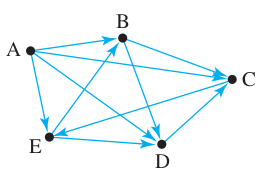
\includegraphics[scale=0.5]{../images/5.3.36.png}
\end{figure}

Use mathematical induction to show that in any round-robin tournament involving $n$ teams, where $n \geq 2$, it is possible to label the teams $T_1, T_2, \ldots, T_n$ so that $T_i$ beats $T_{i + 1}$ for all $i = 1, 2, \ldots, n - 1$. (For instance, one such labeling in the example above is $T_1 = A, T_2 = B, T_3 = C, T_4 = E, T_5 = D$.) ({\it Hint:} Given $k+1$ teams, pick one, say $T'$, and apply the inductive hypothesis to the remaining teams to obtain an ordering $T_1, T_2, \ldots, T_k$. Consider three cases: $T'$ beats $T_1$, $T'$ loses to the first $m$ teams (where $1 \leq m \leq k - 1$) and beats the $(m + 1)$st team, and $T'$ loses to all the other teams.)

\begin{proof}
Let the property $P(n)$ be ``in any round-robin tournament involving $n$ teams, it is possible to label the teams $T_1, T_2, \ldots, T_n$ so that $T_i$ beats $T_{i + 1}$ for all $i = 1, 2, \ldots, n - 1$.''.

{\bf Show that $P(2)$ is true:} In a round-robin tournament with two teams $A, B$, either $A$ beats $B$, in which case label $T_1 = A$ and $T_2 = B$, or $B$ beats $A$, in which case label $T_1 = B$ and $T_2 = A$. So in both cases $T_1$ beats $T_2$. So $P(2)$ is true.

{\bf Show that for every integer $k \geq 2$, if $P(k)$ is true then $P(k+1)$ is true:} Suppose $k \geq 2$ is any integer such that $P(k)$ is true. So in any round-robin tournament involving $k$ teams, it is possible to label the teams $T_1, T_2, \ldots, T_k$ so that $T_i$ beats $T_{i + 1}$ for all $i = 1, 2, \ldots, k - 1$. {\cy $\from P(k)$ inductive hypothesis}

{\it [We want to show that in any round-robin tournament involving $k+1$ teams, it is possible to label the teams $S_1, S_2, \ldots, S_{k+1}$ so that $S_i$ beats $S_{i + 1}$ for all $i = 1, 2, \ldots, k$.]} {\cy $\from P(k+1)$}

Given $k+1$ teams, pick one, say $X$. By the inductive hypothesis applied to the remaining $k$ teams, there exists an ordering $T_1, T_2, \ldots, T_k$ so that $T_i$ beats $T_{i + 1}$ for all $i = 1, 2, \ldots, k - 1$.

{\bf Case 1: $X$ beats $T_1$.} Then label the $k+1$ teams as follows: $S_1 = X, S_2 = T_1, S_3 = T_2, \ldots, S_{k+1} = T_k$. Now $S_i$ beats $S_{i + 1}$ for all $i = 1, 2, \ldots, k$, {\it [as was to be shown.]}

{\bf Case 2: There exists an integer $m$ where $1 \leq m \leq k - 1$ such that $X$ loses to $T_1, T_2, \ldots, T_m$ and beats $T_{m + 1}$.} Then label the $k+1$ teams as follows: $S_1 = T_1, \ldots, S_m = T_m, S_{m+1} = X, S_{m+2} = T_{m+1}, \ldots, S_{k+1} = T_k$. Now $S_i$ beats $S_{i + 1}$ for all $i = 1, 2, \ldots, k$, {\it [as was to be shown.]}

{\bf Case 3: $X$ loses to all the other teams.} Then label the $k+1$ teams as follows: $S_1 = T_1, S_2 = T_2, \ldots, S_k = T_k, S_{k+1} = X$. Now $S_i$ beats $S_{i + 1}$ for all $i = 1, 2, \ldots, k$, {\it [as was to be shown.]}
\end{proof}

\subsection{Exercise 37}
On the outside rim of a circular disk the integers from 1 through 30 are painted in random order. Show that no matter what this order is, there must be three successive integers whose sum is at least 45.

{\it Hint:} Use proof by contradiction. If the statement is false, then there exists some ordering of the integers from 1 to 30, say, $x_1, x_2, \ldots, x_{30}$, such that $x_1 + x_2 + x_3 < 45, x_2 + x_3 + x_4 < 45, \ldots$, and $x_{30} + x_1 + x_2 < 45$. Evaluate the sum of all these inequalities using the fact that $\sum_{i = 1}^{30} x_i = \sum_{i = 1}^{30} i$ and Theorem 5.2.1.

\begin{proof}
(following the Hint)

Argue by contradiction. Assume the statement is false, then there exists some ordering of the integers from 1 to 30, say, $x_1, x_2, \ldots, x_{30}$, such that the following 30 inequalities are true:

$x_1 + x_2 + x_3 < 45$, 

$x_2 + x_3 + x_4 < 45$,

$x_3 + x_4 + x_5 < 45$, 

$\vdots$

$x_{30} + x_1 + x_2 < 45$. 

Notice that for every $i$ with $1 \leq i \leq 30$, the integer $x_i$ occurs exactly 3 times total in all of the inequalities.

Therefore, adding up all these inequalities we get
\[
3x_1 + 3x_2 + \cdots + 3x_{30} < 45 \cdot 30 = 1350.
\]

Since the integers $x_1, \ldots, x_{30}$ are an ordering of the integers $1, \ldots, 30$, we have 
\[
\dps \sum_{i = 1}^{30} x_i = \sum_{i = 1}^{30} i = \frac{30 \cdot 31}{2} = 465.
\] 
It follows that $\dps 3x_1 + \cdots + 3x_{30} = 3\sum_{i = 1}^{30} x_i = 3 \cdot 465 = 1395$. But we also have $3x_1 + \cdots + 3x_{30} < 1350$, so $1395 < 1350$, a contradiction. {\it [Thus our supposition was false, and the original statement is true.]}
\end{proof}

\subsection{Exercise 38}
Suppose that $n$ $a$’s and $n$ $b$’s are distributed around
the outside of a circle. Use mathematical induction to prove that for any integer $n \geq 1$, given any such arrangement, it is possible to find a starting point so that if you travel around the circle in a clockwise direction, the number of $a$’s you pass is never less than the number of $b$’s you have passed. For example, in the diagram shown below, you could start at the $a$ with an asterisk.

\begin{figure}[ht!]
\centering
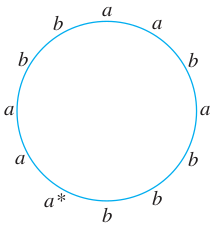
\includegraphics[scale=0.5]{../images/5.3.38.png}
\end{figure}

{\it Hint:} Given $k + 1$ $a$’s and $k + 1$ $b$’s arrayed around the outside of the circle, there has to be at least one location where an $a$ is followed by a $b$ as one travels in the clockwise direction. In the inductive step, temporarily remove such an $a$ and the $b$ that follows it, and apply the inductive hypothesis.

\begin{proof}
Let the property $P(n)$ be ``given $n$ $a$'s and $n$ $b$'s distributed around the outside of a circle, it is possible to find a starting point so that if you travel around the circle in a clockwise direction, the number of $a$'s you pass is never less than the number of $b$'s you have passed.''.

{\bf Show that $P(1)$ is true:} Given one $a$ and one $b$ we can start from the $a$ and go clockwise:

\begin{figure}[ht!]
\centering
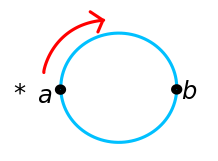
\includegraphics[scale=0.5]{../images/5.3.38.a.png}
\end{figure}

Then the number of $a$'s we pass will be 1 after we pass through the $a$, and the number of $b$'s we have passed at that point is 0, and 1 is not less than 0. So $P(1)$ is true.

{\bf Show that for every integer $k$ with $k \geq 1$, if $P(k)$ is true then $P(k+1)$ is true:} Assume $P(k)$ is true. Assume we are given $k+1$ $a$'s and $k+1$ $b$'s arranged around the outside of a circle.

On the circle, there must be at least one $a$ which is next to a $b$ when we are going clockwise. Removing that $a$ and $b$ leaves us with $k$ $a$'s and $k$ $b$'s. By the inductive hypothesis, it is possible to find a starting point so that if you travel around the circle in a clockwise direction, the number of $a$'s you pass is never less than the number of $b$'s you have passed. Mark this starting point with an asterisk *:

\begin{figure}[ht!]
\centering
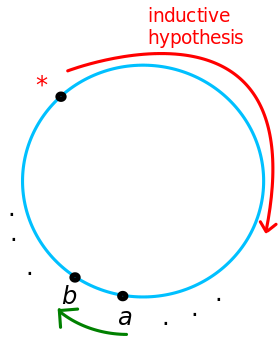
\includegraphics[scale=0.5]{../images/5.3.38.b.png}
\end{figure}

Now if we add back the $a$ and the $b$ that we removed, start from the same point at * and go clockwise, and go over the previously removed $a$ and $b$, it is still true that the number of $a$'s you pass is never less than the number of $b$'s you have passed (because we will pass over the $a$ first). This proves $P(k+1)$, {\it [as was to be shown.]}
\end{proof}

\subsection{Exercise 39}
For a polygon to be convex means that given any two points on or inside the polygon, the line joining the points lies entirely inside the polygon. Use mathematical induction to prove that for every integer $n \geq 3$, the angles of any $n$-sided convex polygon add up to $180(n - 2)$ degrees.

\begin{proof}
Let the property $P(n)$ be: ``the angles of any $n$-sided convex polygon add up to $180(n - 2)$ degrees.''

{\bf Show that $P(3)$ is true:} $P(3)$ says ``the angles of any triangle add up to $180(3 - 2) = 180$ degrees.'' This is true by our knowledge from high school geometry.

{\bf Show that for every integer $k \geq 3$, if $P(k)$ is true then $P(k+1)$ is true:} Suppose $k$ is an integer with $k \geq 3$ and suppose the angles of any $k$-sided convex polygon add up to $180(k - 2)$ degrees. {\it [We want to show that the angles of any $k+1$-sided convex polygon add up to $180(k+1 - 2)$ degrees.]}

Consider any $k+1$-sided convex polygon. Choose any two adjacent edges and connect them with a third edge (see below).

\begin{figure}[ht!]
\centering
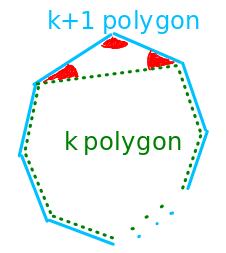
\includegraphics[scale=0.5]{../images/5.3.39.png}
\end{figure}

Since the polygon is convex, this splits the $k+1$-sided polygon (cyan) into two parts: a $k$-sided polygon (green), and a triangle (with red angles). By the inductive hypothesis, the angles of the $k$-sided (green) polygon add up to $180(k - 2)$ degrees. 

Now observe that the sum of the angles of the $k+1$-sided (cyan) polygon is equal to: 

the sum of the angles of the $k$-sided polygon (green) $ = 180(k-2)$

PLUS 

the sum of the angles of the triangle (red) $ = 180$

which equals $180(k-2) + 180 = 180(k+1-2)$ {\it [as was to be shown.]}
\end{proof}

\subsection{Exercise 40}
\subsubsection{(a)}
Prove that in an $8 \times 8$ checkerboard with alternating black and white squares, if the squares in the top right and bottom left corners are removed the remaining board cannot be covered with dominoes. ({\it Hint:} Mathematical induction is not needed for this proof.)

\begin{proof}
Let us consider an $8 \times 8$ checkerboard with alternating black and white squares. Thus, the checkerboard has total 64 squares, with 32 black and 32 white in color. Now, if the squares in the top right and bottom left corners are removed, both the removed ones are either black or white in color. Therefore, out of the remaining 62 squares, 30 squares are of one color and 32 are of other. Now a domino always covers one black and one white square. Thus, the board with 30 of one color and 32 of other cannot be covered with dominoes.
\end{proof}

\subsubsection{(b)}
Use mathematical induction to prove that for each positive integer $n$, if a $2n \times 2n$ checkerboard with alternating black and white squares has one white square and one black square removed anywhere on the board, the remaining squares can be covered with dominoes.

{\it Hint:} In the inductive step, imagine dividing a $2(k + 1) \times 2(k + 1)$ checkerboard into two sections: a center checkerboard of dimensions $2k \times 2k$ and an outer perimeter of single, adjacent squares. Then examine three cases: case 1 is where both removed squares are in the central $2k \times 2k$ checkerboard, case 2 is where one removed square is in the central $2k \times 2k$ checkerboard and the other is on the perimeter, and case 3 is where both removed squares are on the perimeter.

\begin{proof}
Let the property $P(n)$ be: ``if a $2n \times 2n$ checkerboard with alternating black and white squares has one white square and one black square removed anywhere on the board, the remaining squares can be covered with dominoes.''

{\bf Show that $P(1)$ is true:} $P(1)$ says ``if a $2 \times 2$ checkerboard with alternating black and white squares has one white square and one black square removed anywhere on the board, the remaining squares can be covered with dominoes.''

A $2 \times 2$ alternating B \& W board looks like this:
\begin{tabular}{|c|c|}
\hline
\colsq{black} & \colsq{lightgray} \\
\hline
\colsq{lightgray} & \colsq{black} \\
\hline
\end{tabular}
This means that, if one white square and one black square are removed, then either a row or a column is removed. So the remaining row or column can be covered with one domino. So $P(1)$ is true.

{\bf Show that for every integer $k \geq 1$, if $P(k)$ is true then $P(k+1)$ is true:} Assume $k \geq 1$ is an integer such that if a $2k \times 2k$ checkerboard with alternating black and white squares has one white square and one black square removed anywhere on the board, the remaining squares can be covered with dominoes.

{\it [We want to show that if a $2(k+1) \times 2(k+1)$ checkerboard with alternating black and white squares has one white square and one black square removed anywhere on the board, the remaining squares can be covered with dominoes.]}

(following the Hint) Split the $2(k+1) \times 2(k+1)$ board into two sections: a $2k \times 2k$ center, and the remaining perimeter surrounding it. For example, if $k = 3$ then it looks like this (for demonstration purposes, I colored the center yellow and the perimeter blue):

\begin{center}
\begin{tabular}{|c|c|c|c|c|c|c|c|}
\hline
\colsq{blue} & \colsq{blue} & \colsq{blue} & \colsq{blue} & \colsq{blue} & \colsq{blue} & \colsq{blue} & \colsq{blue}\\
\hline
\colsq{blue} & \colsq{yellow} & \colsq{yellow} & \colsq{yellow} & \colsq{yellow} & \colsq{yellow} & \colsq{yellow} & \colsq{blue}\\
\hline
\colsq{blue} & \colsq{yellow} & \colsq{yellow} & \colsq{yellow} & \colsq{yellow} & \colsq{yellow} & \colsq{yellow} & \colsq{blue}\\
\hline
\colsq{blue} & \colsq{yellow} & \colsq{yellow} & \colsq{yellow} & \colsq{yellow} & \colsq{yellow} & \colsq{yellow} & \colsq{blue}\\
\hline
\colsq{blue} & \colsq{yellow} & \colsq{yellow} & \colsq{yellow} & \colsq{yellow} & \colsq{yellow} & \colsq{yellow} & \colsq{blue}\\
\hline
\colsq{blue} & \colsq{yellow} & \colsq{yellow} & \colsq{yellow} & \colsq{yellow} & \colsq{yellow} & \colsq{yellow} & \colsq{blue}\\
\hline
\colsq{blue} & \colsq{yellow} & \colsq{yellow} & \colsq{yellow} & \colsq{yellow} & \colsq{yellow} & \colsq{yellow} & \colsq{blue}\\
\hline
\colsq{blue} & \colsq{blue} & \colsq{blue} & \colsq{blue} & \colsq{blue} & \colsq{blue} & \colsq{blue} & \colsq{blue}\\
\hline
\end{tabular}
\end{center}

Now consider the possibilities for the two removed squares.

{\bf Case 1: both removed squares are in the center.} Then by the inductive hypothesis, the $2k \times 2k$ center part with two squares removed (one white, one black) can be completely covered with dominoes. 

The perimeter can also be covered with dominoes: the top and bottom rows each have length $2(k+1)$ consisting of $k+1$ white squares and $k+1$ black squares, so they can be covered with $k+1$ dominoes each, and the remaining sides each have length $2k$ with $k$ white and $k$ black squares, which can be covered with $k$ dominoes each. 

Therefore the whole $2(k+1) \times 2(k+1)$ board (with one black, one white square removed) can be covered with dominoes, {\it [as was to be shown.]}

{\bf Case 2: both removed squares are on the perimeter.} The center $2k \times 2k$ part can be covered with dominoes since it has nothing removed. Now since one black and one white square are removed from the perimeter, the two ``paths'' along the perimeter between the two removed squares must each have even lengths, each containing equal numbers of white and black squares. 

For example, in the following picture the removed squares are shown as ``B'' and ``W'' and the others are shown in black and white, except the center which is not shown:

\begin{center}
\begin{tabular}{|c|c|c|c|c|c|c|c|}
\hline
\colsq{black} & \colsq{lightgray} & \colsq{black} & \colsq{lightgray} & \colsq{black} & \colsq{lightgray} & \colsq{black} & \colsq{lightgray} \\
\hline
\colsq{lightgray} &  &  &  &  &  &  & \colsq{black} \\
\hline
B &  &  &  &  &  &  & \colsq{lightgray} \\
\hline
\colsq{lightgray} &  &  &  &  &  &  & \colsq{black} \\
\hline
\colsq{black} &  &  &  &  &  &  & \colsq{lightgray} \\
\hline
\colsq{lightgray} &  &  &  &  &  &  & \colsq{black} \\
\hline
\colsq{black} &  &  &  &  &  &  & \colsq{lightgray} \\
\hline
\colsq{lightgray} & \colsq{black} & \colsq{lightgray} & \colsq{black} & \colsq{lightgray} & \colsq{black} & W & \colsq{black} \\
\hline
\end{tabular}
\end{center}

So both of those ``paths'' can be covered by dominoes, since they have even lengths, no gaps, and equal numbers of white and black squares. Hence the whole $2(k+1) \times 2(k+1)$ board can be covered, {\it [as was to be shown.]}

{\bf Case 3: one removed square is in the center, the other on the perimeter.} Consider the two squares removed, say P is removed from the perimeter, and C is removed from the center. 

If P and C are close enough to each other, so that they are both inside a $2k \times 2k$ square (not the center but some other $2k \times 2k$ square), then by the inductive hypothesis, that $2k \times 2k$ square can be covered with dominoes, and the remaining portion of the $2(k+1) \times 2(k+1)$ square can also be covered with dominoes since it has equal numbers of white and black squares, and no gaps. Here is an example with $k = 3$:

\begin{figure}[ht!]
\centering
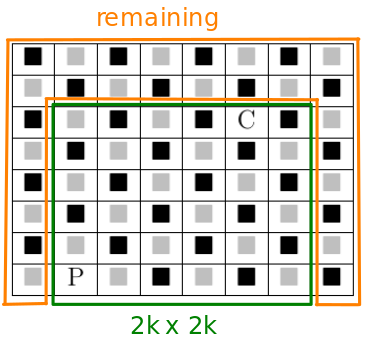
\includegraphics[scale=0.5]{../images/5.3.40.b.1.png}
\end{figure}

So we may assume that P and C do not fall into a $2k \times 2k$ square. In other words, we may assume that C is at the opposite end of the center from P, so that either horizontally or vertically, there are $2k-1$ squares between P and C. 

Since P and C have different colors, they cannot be on the same diagonal, so P and C always fit inside a $2k \times (2k+1)$ or a $(2k+1) \times 2k$ rectangle. Here are some examples for $k = 1$ to illustrate this. They always fit into either a $2 \times 3$ or a $3 \times 2$ rectangle:

\begin{figure}[ht!]
\centering
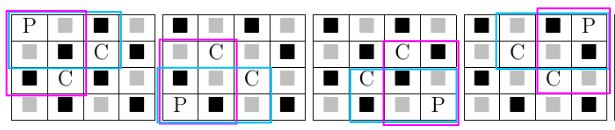
\includegraphics[scale=0.6]{../images/5.3.40.b.2.png}
\end{figure}

We cannot apply the inductive hypothesis to this $2k \times (2k+1)$ or $(2k+1) \times 2k$ rectangle. So we have to move C closer to P by one diagonal, so that the horizontal or vertical distance is $2k-2$ and hence they fall into a $2k \times 2k$ square. Here is an example for $k = 2$:

\begin{figure}[ht!]
\centering
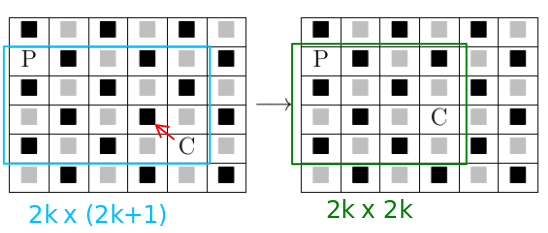
\includegraphics[scale=0.5]{../images/5.3.40.b.3.png}
\end{figure}

(Of course, depending on the position of P, we might have to move C in any one of the 4 diagonal directions. The picture above is only one example.)

Now we have to show that, this $2k \times (2k+1)$ or $(2k+1) \times 2k$ rectangle can be covered by dominoes, if and only if, the $2k \times 2k$ square obtained by moving C diagonally closer to P can be covered by dominoes. (This is possible but the proof is annoying and complicated, so I'll skip it here.)

By the inductive hypothesis, any $2k \times 2k$ board with one white and one black square removed can be covered with dominoes. Thus, by the above ``if and only if'' equivalence, the $2k \times (2k+1)$ or $(2k+1) \times 2k$ board can also be covered by dominoes. The remaining portion of the $2(k+1) \times 2(k+1)$ board can also be covered by dominoes, like before. So the whole $2(k+1) \times 2(k+1)$ board can be covered by dominoes, {\it [as was to be shown.]}
\end{proof}

\subsection{Exercise 41}
A group of people are positioned so that the distance between any two people is different from the distance between any other two people. Suppose that the group contains an odd number of people and each person sends a message to their nearest neighbor. Use mathematical induction to prove that at least one person does not receive a message from anyone. [This exercise is inspired by the article “Odd Pie Fights” by L. Carmony, The Mathematics Teacher, 72(1), 1979, 61–64.]

{\it Hint:} Let $P(n)$ be the sentence: If (1) $2n + 1$ people are all positioned so that the distance between any two people is different from the distance between any two other people, and if (2) each person sends a message to their nearest neighbor, then there is at least one person who does not receive a message from anyone. Use mathematical induction to prove that $P(n)$ is true for each integer $n \geq 1$.

\begin{proof}
(following the Hint) Let $P(n)$ be the sentence: ``If (1) $2n + 1$ people are all positioned so that the distance between any two people is different from the distance between any two other people, and if (2) each person sends a message to their nearest neighbor, then there is at least one person who does not receive a message from anyone.''

{\bf Show that $P(0)$ is true:} $P(0)$ says: ``If (1) $2 \cdot 0 + 1$ people are all positioned so that the distance between any two people is different from the distance between any two other people, and if (2) each person sends a message to their nearest neighbor, then there is at least one person who does not receive a message from anyone.'' 

Now the group has only $2 \cdot 0 + 1 = 1$ person and this person does not receive a message from anyone. So $P(0)$ is true.

{\bf Show that for every integer $k \geq 0$ if $P(k)$ is true then $P(k+1)$ is true:}

Suppose $k\geq 0$ is an integer such that $P(k)$ is true: if (1) $2k + 1$ people are all positioned so that the distance between any two people is different from the distance between any two other people, and if (2) each person sends a message to their nearest neighbor, then there is at least one person who does not receive a message from anyone. {\it [We want to show $P(k+1)$ is true.]}

To prove $P(k+1)$, suppose (1) $2(k+1) + 1$ people are all positioned so that the distance between any two people is different from the distance between any two other people, and (2) each person sends a message to their nearest neighbor.

{\it [Then we want to show there is at least one person who does not receive a message from anyone.]}

{\it [how to continue ??? Remove two people, use inductive hypothesis?]}
\end{proof}

\subsection{Exercise 42}
Show that for any (positive) even integer $n$, it is possible to find a group of $n$ people who are all positioned so that the distance between any two people is different from the distance between any other two people, so that each person sends a message to their nearest neighbor, and so that every person in the group receives a message from another person in the group.

\begin{proof}
{\it ???}
\end{proof}

\subsection{Exercise 43}
Define a game as follows: You begin with an urn that contains a mixture of white and black balls, and during the game you have access to as many additional white and black balls as you might need. In each move you remove two balls from the urn without looking at their colors. If the balls
are the same color, you put in one black ball. If the balls are different colors, you put the white ball back into the urn and keep the black ball out. Because each move reduces the number of balls in the urn by one, the game will end with a single ball in the urn. If you know how many white balls and how many black balls are initially in the urn, can you predict the color of the ball at the end of the game? [This exercise is based on one described in “Why correctness must be a mathematical concern” by E. W. Dijkstra, www.cs.utexas.edu/users /EWD/transcriptions/EWD07xx/EWD720.html.]

\subsubsection{(a)}
Map out all possibilities for playing the game starting with two balls in the urn, then three balls, and then four balls. For each case keep track of the number of white and black balls you start with and the color of the ball at the
end of the game.

{\it Hint:}
\arrayrulecolor{cyan}
\begin{tabular}{|ccc|}
\hline
\multicolumn{3}{|c|}{\cy Two Balls} \\
\hline
WW & $\to$ & B \\
\hline
WB & $\to$ & W \\
\hline
BB & $\to$ & B \\
\hline
\end{tabular}
\begin{tabular}{|cc|cc|}
\hline
\multicolumn{4}{|c|}{\cy Summary} \\
\hline
\multicolumn{2}{|c|}{Start} & \multicolumn{2}{c|}{End} \\
\hline
W & B & W & B \\
\hline
2 & 0 & 0 & 1 \\
\hline
1 & 1 & 1 & 0 \\
\hline
0 & 2 & 0 & 1 \\
\hline
\end{tabular}
\arrayrulecolor{black} % change it back!

\begin{proof}
{\it ???}
\end{proof}

\subsubsection{(b)}
Does the number of white balls seem to be predictive? Does the number of black balls seem to be predictive? Make a conjecture about the color of the ball at the end of the game given the numbers of white and black balls at the beginning.

{\it Hint:} In all three cases when the urn initially contains an odd number of white balls, there is one white ball in the urn at the end of the game, and when the urn initially contains an even number of white balls, there is one black ball (i.e., zero white balls) in the urn at the end of the game.

\begin{proof}
{\it ???}
\end{proof}

\subsubsection{(c)}
Use mathematical induction to prove the conjecture you made in part (b).

\begin{proof}
{\it ???}
\end{proof}

\subsection{Exercise 44}
Let $P(n)$ be the following sentence: Given any graph $G$ with $n$ vertices satisfying the condition that every vertex of $G$ has degree at most $M$, then the vertices of $G$ can be colored with at most $M + 1$ colors in such a way that no two adjacent vertices have the same color. Use mathematical induction to prove this statement is true for every integer $n \geq 1$.

{\it Hint:} Given a graph $G$ satisfying the given condition, form a new graph $G'$ by deleting one vertex $v$ of $G$ and all the edges that are incident on $v$. Then apply the inductive hypothesis to $G'$.

\begin{proof}
{\bf Show that $P(1)$ is true:} Given any graph $G$ with 1 vertex satisfying the given condition, we can color this vertex with only 1 color (which is $\leq M+1$) so that no two adjacent vertices have the same color (since there are no two adjacent vertices at all). So $P(1)$ is true.

{\bf Show that for any integer $k \geq 1$, if $P(k)$ is true then $P(k+1)$ is true:} Assume $P(k)$ is true, {\it [we want to prove $P(k+1)$ is true].} To prove $P(k+1)$ assume $G$ is any graph with $k+1$ vertices with degree at most $M$. {\it [We want to show that the vertices of $G$ can be colored with at most $M+1$ colors so that no two adjacent vertices have the same color.]}


Form a new graph $G'$ by deleting one vertex $v$ of $G$ and all the edges that are incident on $v$. Now $G'$ has $k$ vertices with degree at most $M$. By the inductive hypothesis we can color the vertices of $G'$ with at most $M+1$ colors so that no two adjacent vertices have the same color.

{\it ???}
\end{proof}

{\bf \cy In order for a proof by mathematical induction to be valid, the basis statement must be true for $n = a$ and the argument of the inductive step must be correct for every integer $k \geq a$. In 45 and 46 find the mistakes in the “proofs” by mathematical induction.}

\subsection{Exercise 45}
{\bf “Theorem:”} For any integer $n \geq 1$, all the numbers in a set of n numbers are equal to each other.

{\bf “Proof (by mathematical induction):} It is obviously true that all the numbers in a set consisting of just one number are equal to each other, so the basis step is true. For the inductive step, let $A = \{a_1, a_2, \ldots, a_k, a_{k+1}\}$ be any set of $k + 1$ numbers. Form two subsets each of size $k$:
\[
B = \{a_1, a_2, a_3, \ldots, a_k\} \text{ and } C = \{a_1, a_3, a_4, \ldots, a_{k+1}\}.
\]
($B$ consists of all the numbers in $A$ except $a_{k+1}$, and $C$ consists of all the numbers in $A$ except $a_2$.) By inductive hypothesis, all the numbers in $B$ equal $a_1$ and all the numbers in $C$ equal $a_1$ (since both sets have only $k$ numbers). But every number in $A$ is in $B$ or $C$, so all the numbers in $A$ equal $a_1$; hence all are equal to each other.”

\begin{proof}
The inductive step fails for going from $n = 1$ to $n = 2$,
because when $k = 1$,
\[
A = \{a_1, a_2\} \text{ and } B = \{a_1\}
\]
and no set $C$ can be defined to have the properties claimed for the $C$ in the proof. The reason is that $C = \{a_1\} = B$, and so an element of $A$, namely $a_2$, is
not in either $B$ or $C$.

Since the inductive step fails for going from $n = 1$ to $n = 2$, the truth of the following statement is never proved: “All the numbers in a set of two numbers are equal to each other.” This breaks the sequence of inductive steps, and so none of the statements for $n > 2$ is proved true either.

Here is an explanation for what happens in terms of the
domino analogy. The first domino is tipped backward (the basis step is proved). Also, if any domino from the second onward tips backward (the inductive step works or $n \geq 2$). In this case, however, when the first domino is tipped backward, it does not tip the second domino backward. So only the first domino falls down; the rest remain standing.
\end{proof}

\subsection{Exercise 46}
{\bf “Theorem:”} For every integer $n \geq 1$, $3^n - 2$ is even. 

{\bf “Proof (by mathematical induction):} Suppose the theorem is true for an integer $k$, where $k \geq 1$. That is, suppose that $3^k - 2$ is even. We must show that $3^{k+1} - 2$ is even. Observe that $3^{k+1} - 2 = 3^k \cdot 3 - 2 = 3^k(1 + 2) - 2 = (3^k - 2) + 3^k \cdot 2$. Now $3^k - 2$ is even by inductive hypothesis and $3^k \cdot 2$ is even by inspection. Hence the sum of the two quantities is even (by Theorem 4.1.1). It follows that $3^{k+1} - 2$ is even, which is what we needed to show.”

{\it Hint:} Is the basis step true?

\begin{proof}
This proof starts at the inductive step, assuming $P(k)$ and proving $P(k+1)$. However, it does not prove the basis step. In fact, the basis step is false: when $n = 1$, $3^n - 2 = 3^1 - 2 = 1$ is odd.

(Even if the basis step were true, the proof is still incomplete as it's missing the basis step.)
\end{proof}

\end{document}
